\section{\texorpdfstring{Search for \ttH\ production}{Search for ttH production}}
The measurement of the production \xsec\ of the \ttH\ process allows probing directly the top Yukawa coupling.
Indirect constrains on the coupling can be extracted through the measurement of the Higgs production rates~\cite{ATLAS-CONF-2015-007}, 
although with strong assumptions: only SM particles contribute to the loops (see figures~\ref{fig:eff_vtx_ggH} and~\ref{fig:eff_vtx_Hgaga}) and the total Higgs boson width is fixed to the SM value.
A precision of \unit[20]{\%} on the top Yukawa coupling is achieved through this indirect measurement.

The direct measurement of the coupling through the tree-level \ttH\ process (see figure~\ref{fig:eff_vtx_ttH}) allows removing the assumption, in order to disentangle possible new physics contributions in the effective $ggH$ and $\gamma\gamma H$ vertices.

\begin{figure}[htb!]
  \centering
  \begin{subfigure}{0.32\textwidth}
  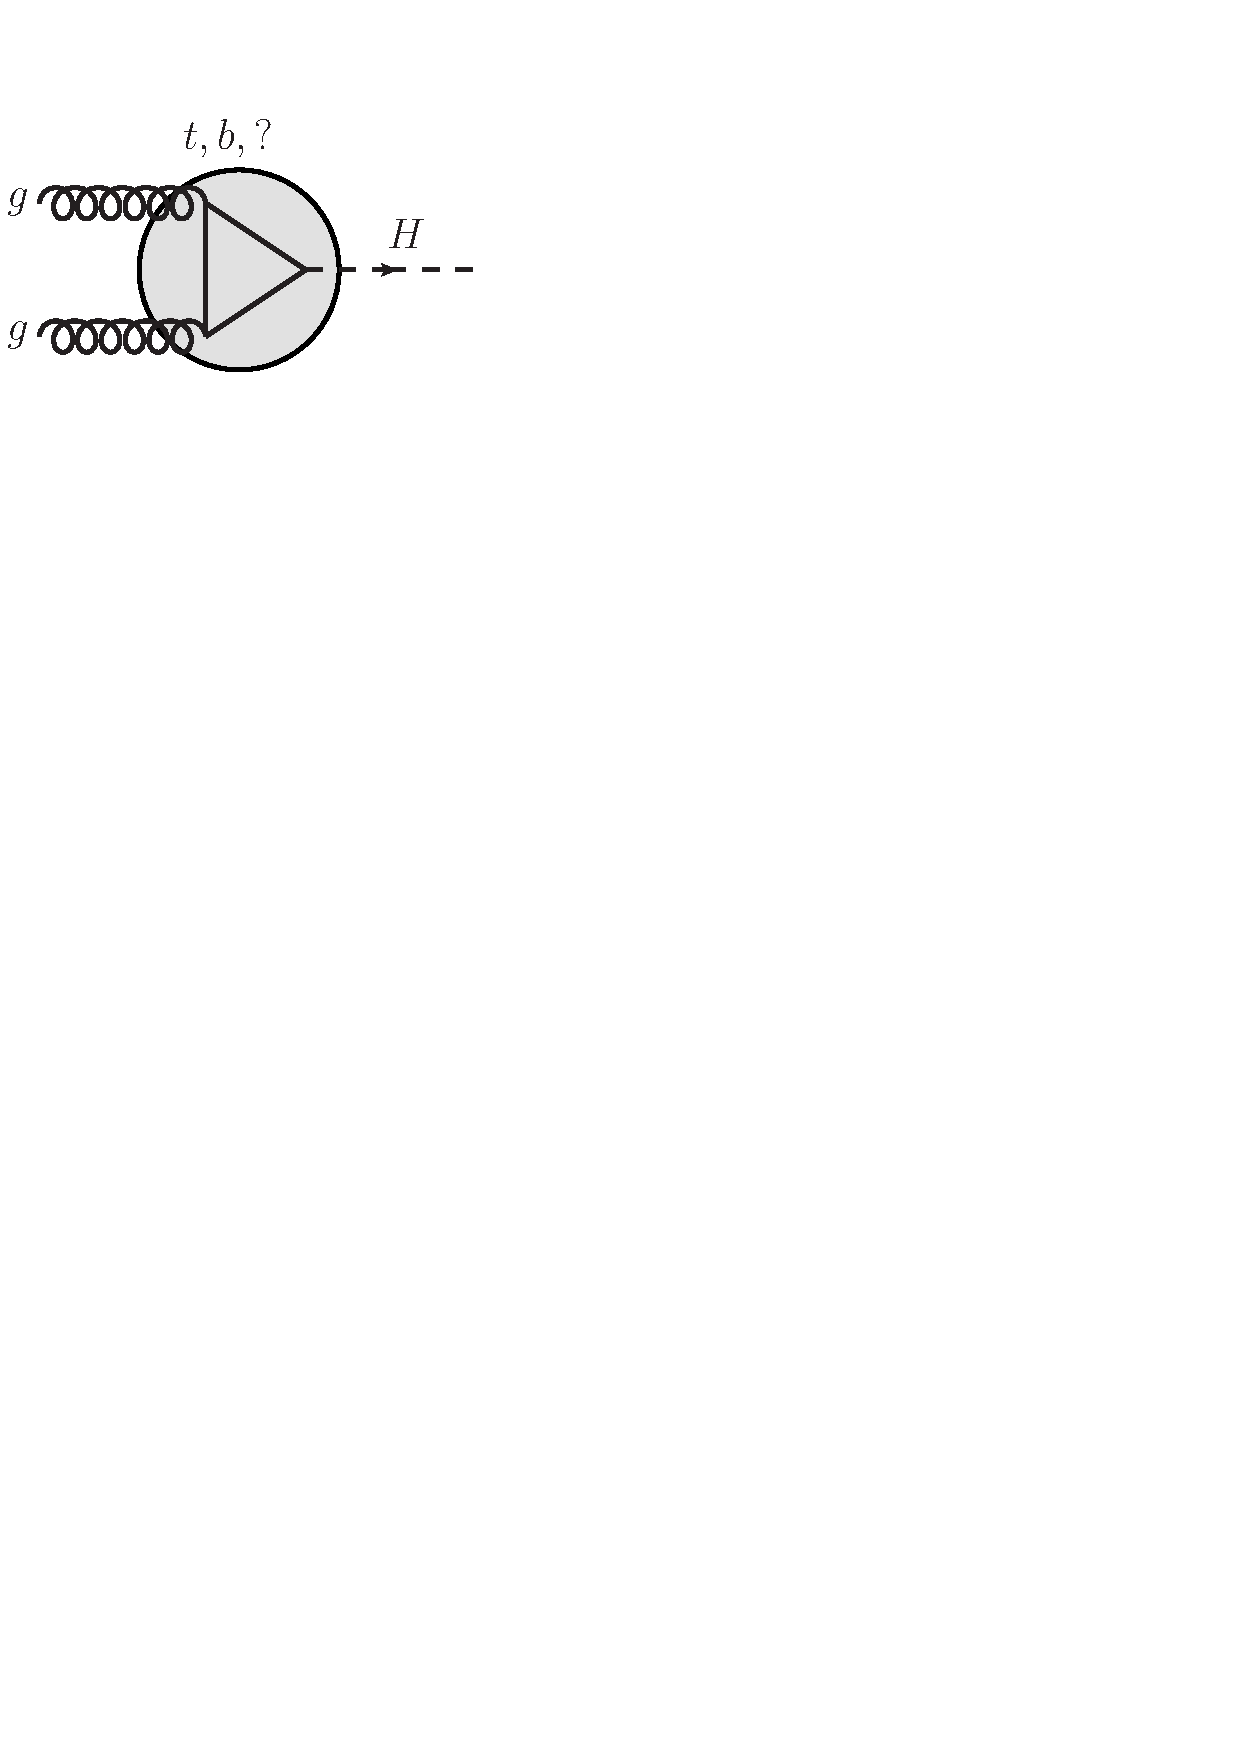
\includegraphics[trim=0cm 22cm 12cm 0.5cm, clip=true, width=0.95\textwidth]{Analysis/Figures_ttH/ggH.pdf}
  \caption{}\label{fig:eff_vtx_ggH}\end{subfigure}
  \begin{subfigure}{0.32\textwidth}
  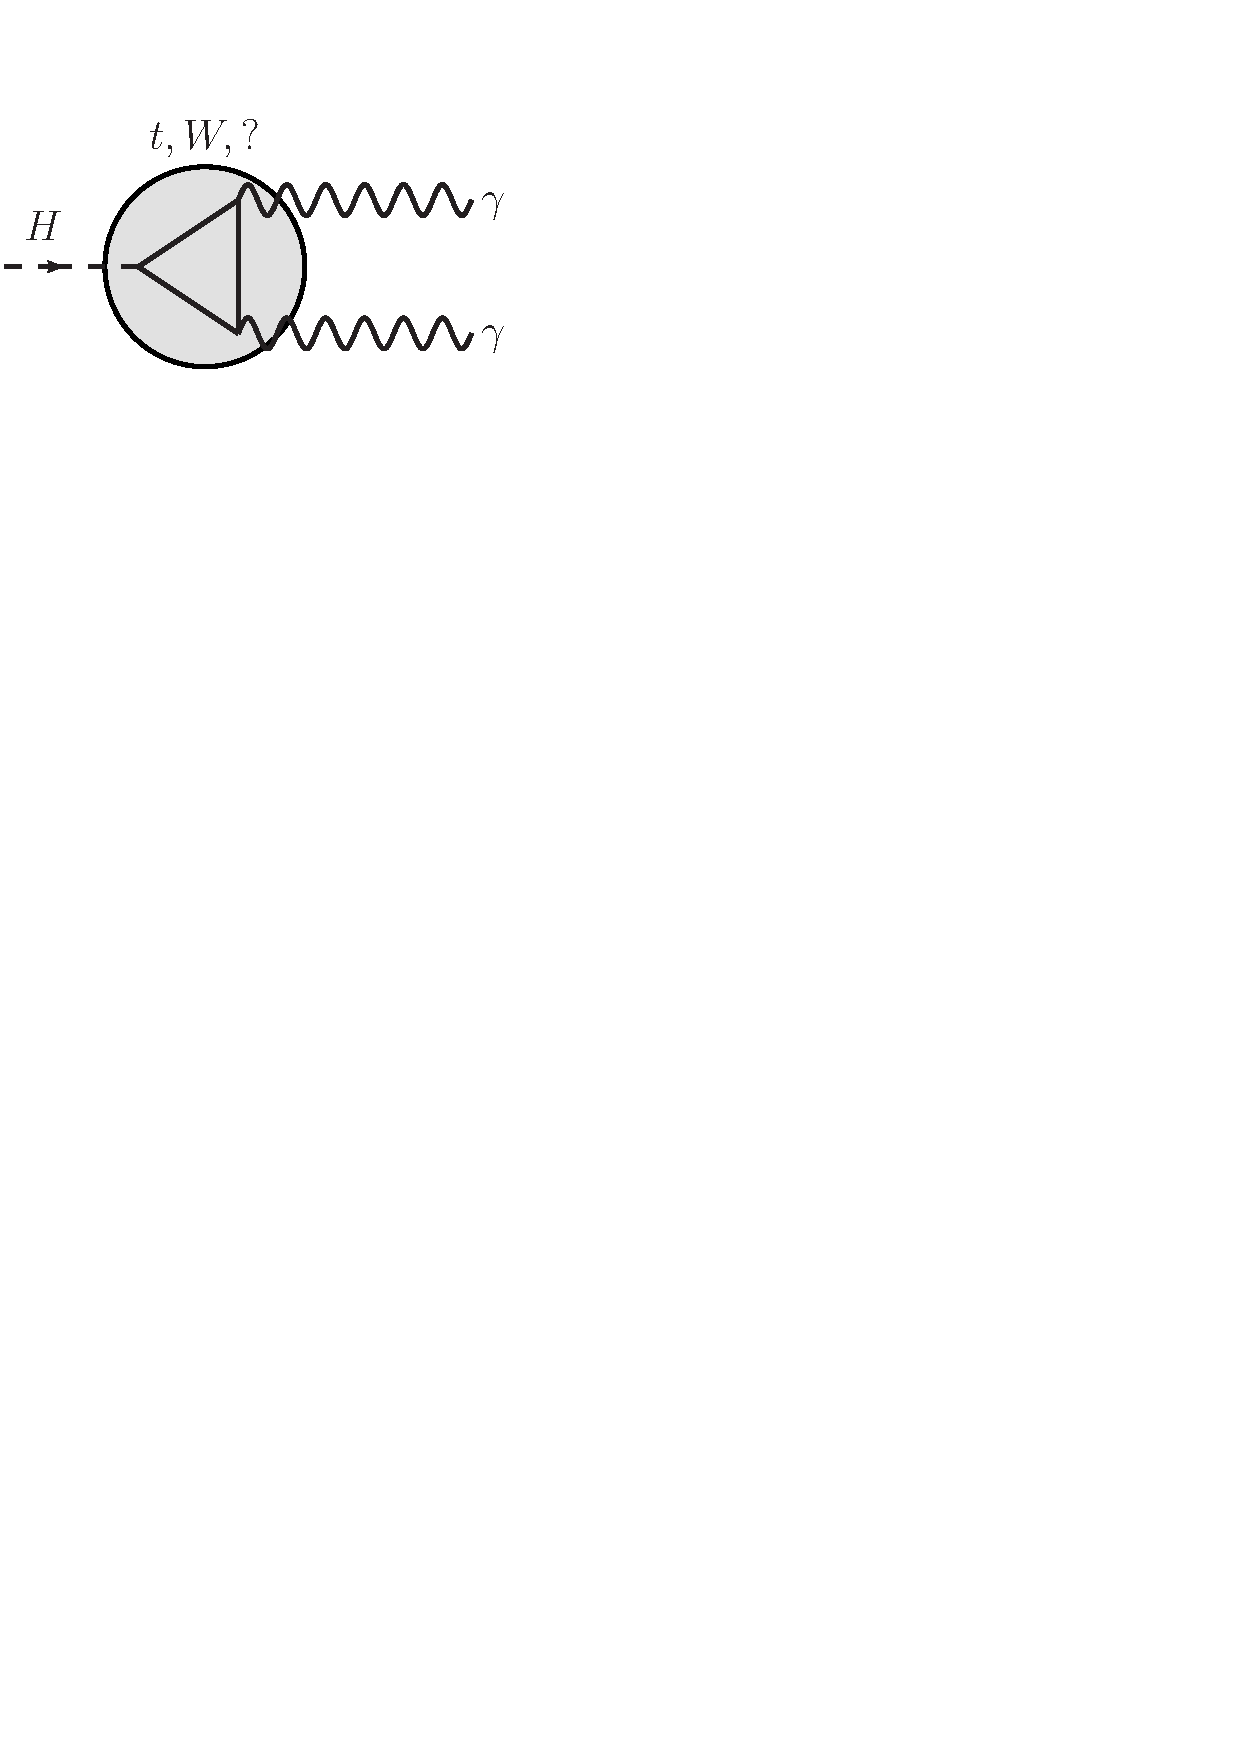
\includegraphics[trim=0cm 22cm 12cm 0.5cm, clip=true, width=0.95\textwidth]{Analysis/Figures_ttH/Hgaga.pdf}
  \caption{}\label{fig:eff_vtx_Hgaga}\end{subfigure}
  \begin{subfigure}{0.32\textwidth}
  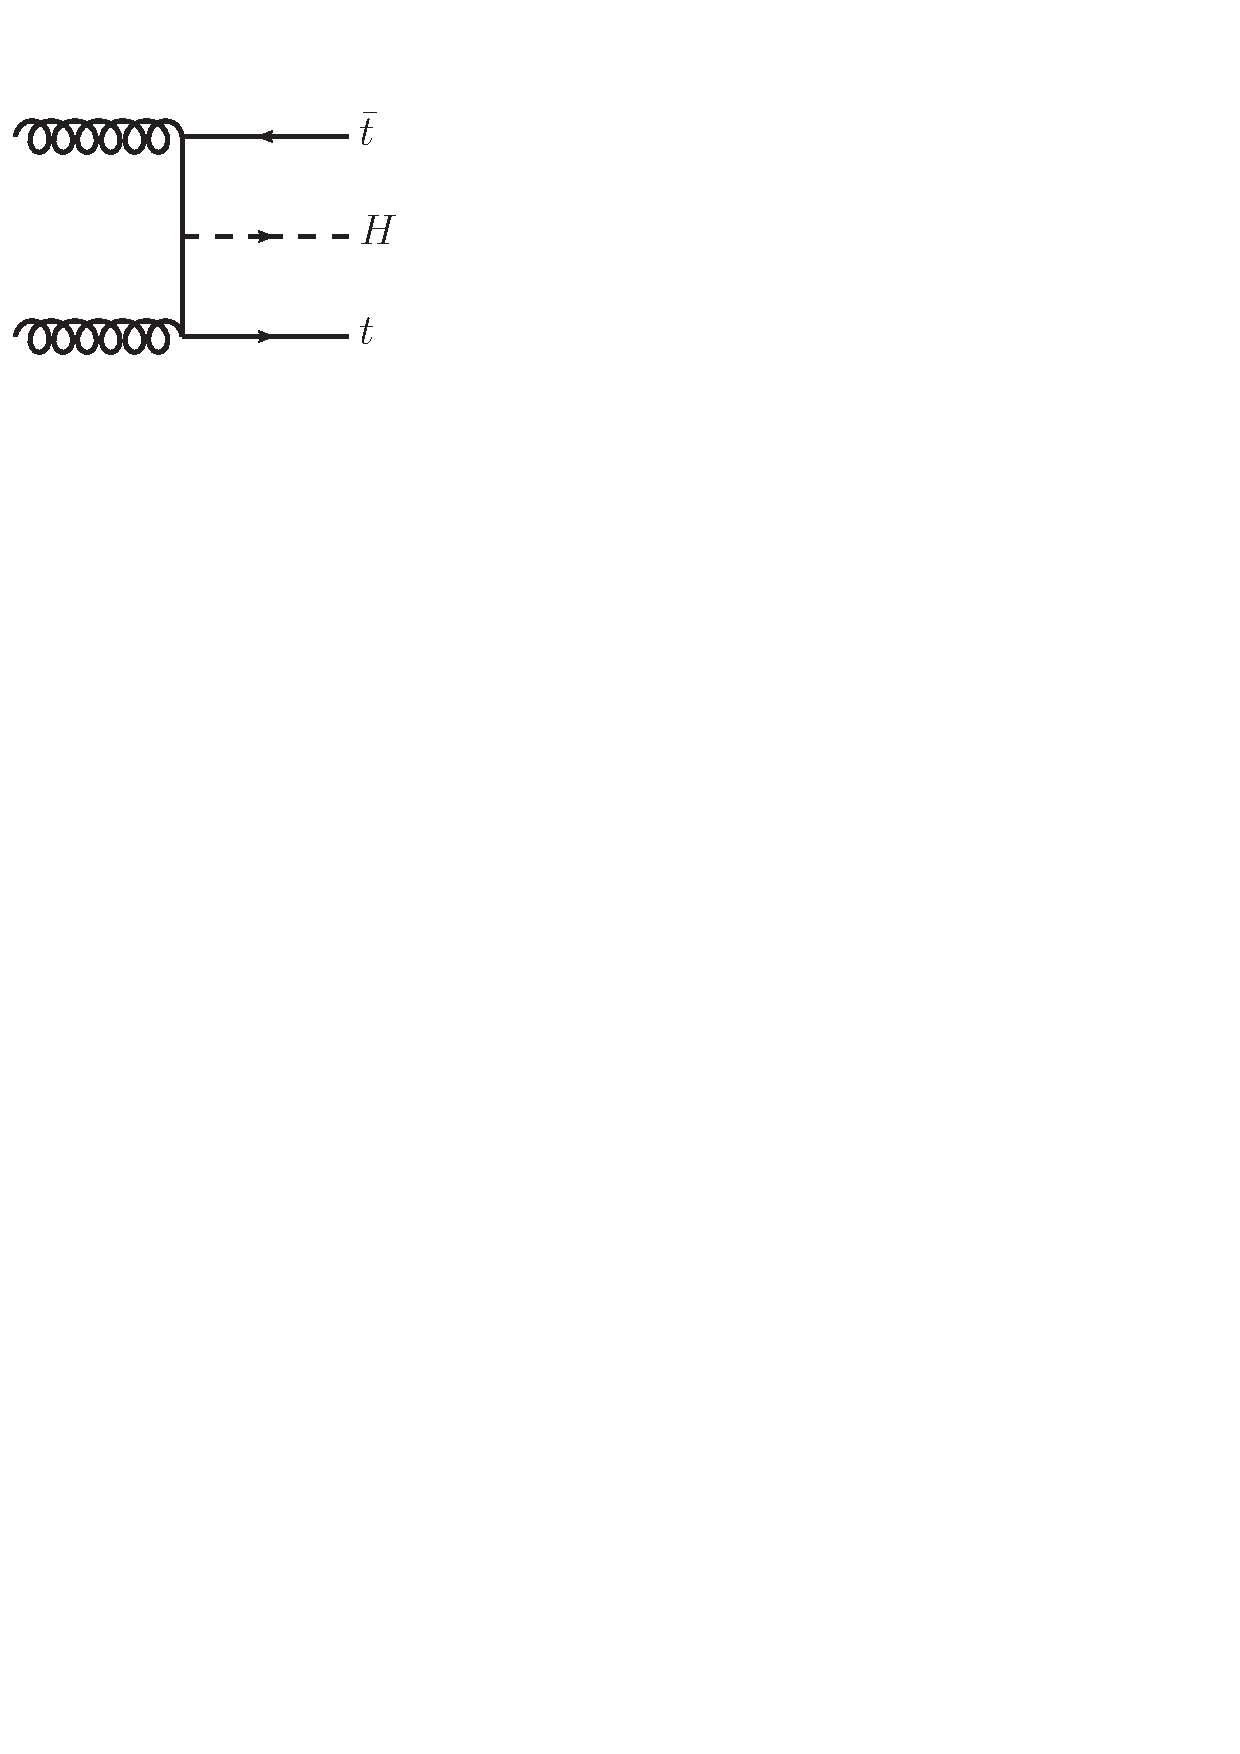
\includegraphics[trim=0cm 22.5cm 12cm 0cm, clip=true, width=0.95\textwidth]{Analysis/Figures_ttH/ttH.pdf}
  \caption{}\label{fig:eff_vtx_ttH}\end{subfigure}
\caption{Example Feynman diagram for (a) the effective gluon fusion vertex $ggH$, (b) the effective photon vertex $\gamma\gamma H$, and (c) the \ttH\ process.}
  \label{fig:eff_vtx}
\end{figure}
\subsection{Event selection and categorization}
After the preselection described in section~\ref{sec:preselection}, the events are categorized in different channels
depending on the number of jets (4, 5 and $\geq$6) and on the number of $b$-tagged jets (2, 3 and $\geq$4).
This categorization allows separating signal-rich regions at high jet and $b$-tag multiplicity from the dominant \ttbar+jets background.
However, after the categorization it becomes very difficult to devise further selection cuts that would allow the suppression of the irreducible \ttbb\ background. One of the characteristics that could allow differentiating the signal from the background is the resonance produced by the decay $H \to \bbbar$. However, the identification of the correct \bbbar\ pair is not trivial, since there are six possible ways of assigning a \bbbar\ pair to the Higgs boson from the four $b$-tagged jets. Previous results in the search for \ttH, $H\to\bbbar$ have followed this approach~\cite{ATLAS2011ttH}, performing a kinematic fit of the final state in order to identify the \ttbar\ system and the Higgs boson candidate. The correct \bbbar\ pairing is only achieved approximately $\unit[20]{\%}$ of the times, while the other $\sim \unit[80]{\%}$ a wrong pairing is chosen,\footnote{A wrong pairing can also be due to acceptance effects, where the products from the Higgs boson decay are not present in the event.}
therefore diluting the expected peak in a combinatorial background.
The matching performance and the expected $m_{\bbbar}$ distribution in \pp\ collisions at $\sqrt{s} = \unit[7]{\tev}$ is shown in figure~\ref{fig:klf_mbb}.
Given the difficulties to isolate the Higgs boson resonance, no selection cut is attempted on this observable. This feature will however be used later in the construction of the discriminant variable.
\begin{figure}[tb!]
  \centering
  \begin{subfigure}{0.49\textwidth}
  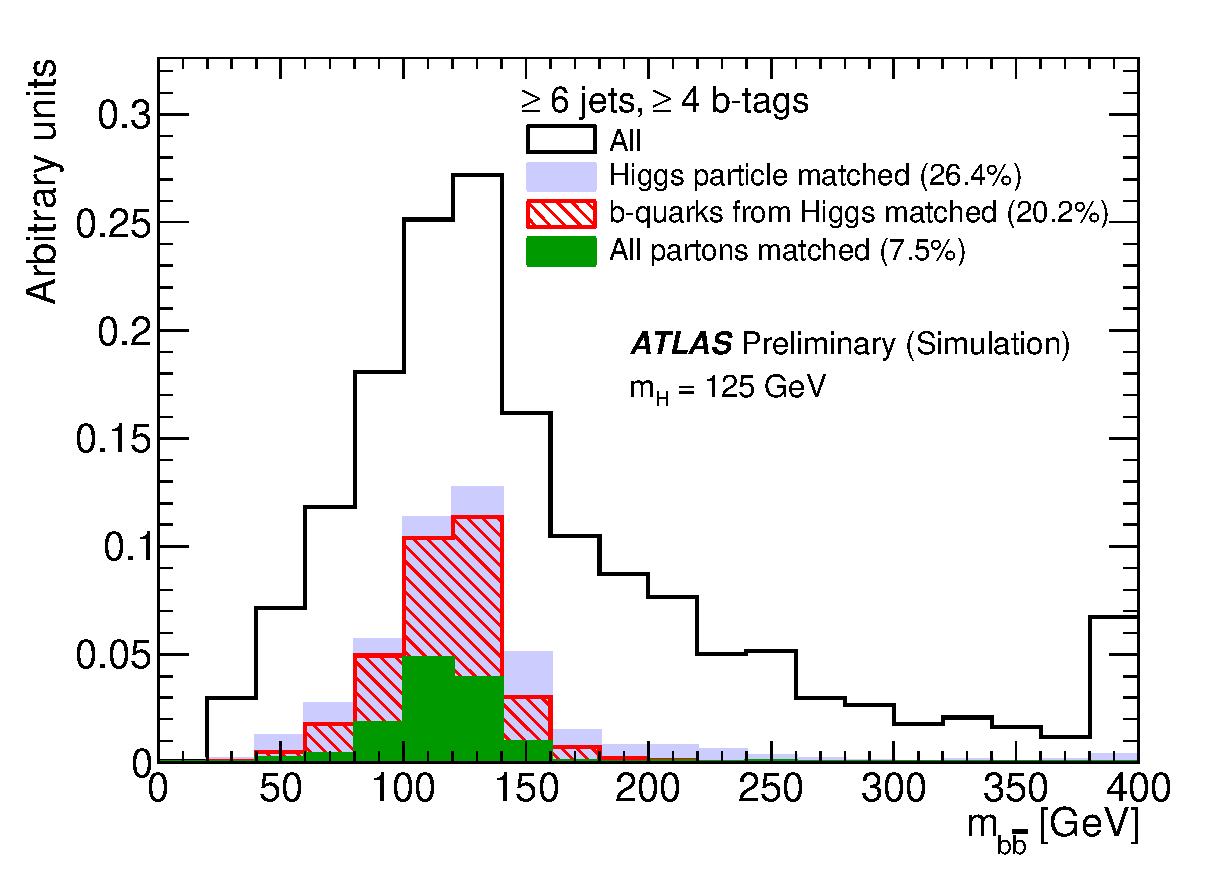
\includegraphics[width=\textwidth]{Analysis/Figures_ttH/fig_03b}
  \caption{} \label{fig:klf_matching} \end{subfigure}
  \begin{subfigure}{0.49\textwidth}
  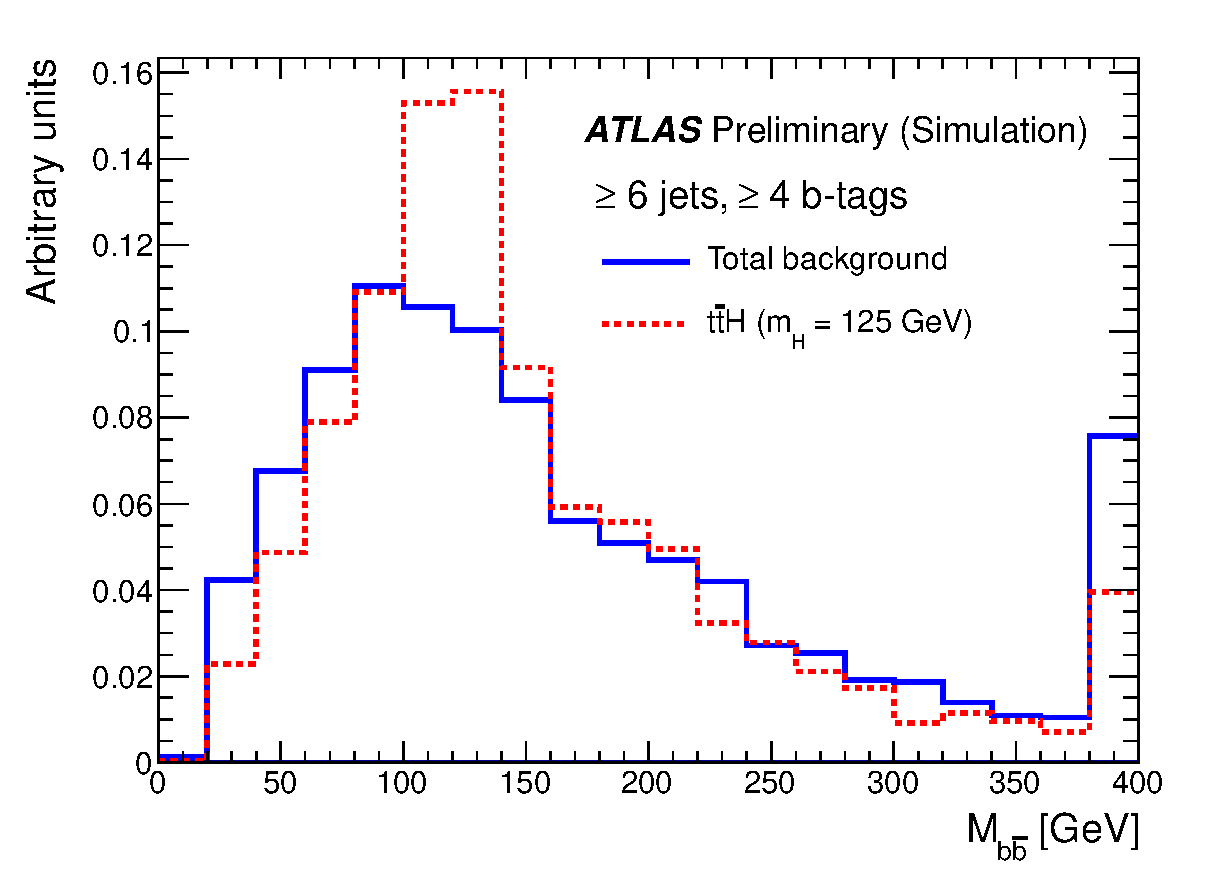
\includegraphics[width=\textwidth]{Analysis/Figures_ttH/fig_04b}
  \caption{} \label{fig:klf_shape} \end{subfigure}
  \caption{
    (a) Distribution of the reconstructed Higgs boson mass ($m_{\bbbar}$) after kinematic fit for simulated \ttH\ signal in the \sixfour\ region.
    Also overlaid are the distributions for the subset of events where the reconstructed Higgs boson matches the generator-level Higgs boson particle (labeled as ``Higgs particle matched''), the subset of events where the two $b$-jets used for $m_{\bbbar}$ match the $b$-quarks from the Higgs boson decay (labeled as ``b quarks from Higgs matched), and the subset of events where all jets considered in the kinematic fit match the partons from the decays of the top quarks and Higgs
  boson (labeled as ''all partons matched``). In all instances angular matching is performed by requiring $\DR <0.4$. 
  (b) 
  Comparison of the $m_{\bbbar}$ distribution between \ttH\ signal (dashed red histogram) and total background (solid blue histogram) in the  \sixfour\ region. Both distributions are normalized to unity in order to better compare the shapes between signal and background.
  }
  \label{fig:klf_mbb}
\end{figure}

The presence of a leptonic $W$ boson is usually exploited in \ttbar\ final states in order to reduce the non-\ttbar\ backgrounds. Selection cuts on kinematics variables such as \met\ or \mtw\ are a common choice, however in the search for \ttH\ these cuts are not included. 
Considering the small \xsec\ of the \ttH\ process, and since 
the efficiency of the cuts is very similar for the signal and the \ttbar\ background, the introduction of these cuts results in a reduction of the sensitivity. This conclusion is reached easily when the sensitivity is estimated as $S/\sqrt{B}$, but it has been also verified with the full systematic model.
The suppression of the non-\ttbar\ backgrounds is already achieved through the requirement of high $b$-tag multiplicity, therefore no further cuts are applied in order to maximize the signal acceptance.

\subsection{Discriminant variable: artificial neural networks}
Given the difficulty to increase the purity of the signal-rich regions, the sensitivity has to be optimized introducing a powerful discriminating variable. 
Artificial Neural Networks (NN) are used to discriminate potential signal events 
from the background. 
They are particularly useful in cases where no single variable exhibits a 
clear separation power between signal and background.
A NN allows combining the information from several input variables into one output discriminant that exploits the correlations among the variables and can reproduce a non-trivial selection in the variables' phase space.
The present analysis is an ideal ground for the application of such a 
multivariate approach given the large number of physics objects in the 
final state.

\begin{figure}[tb!]
  \centering
  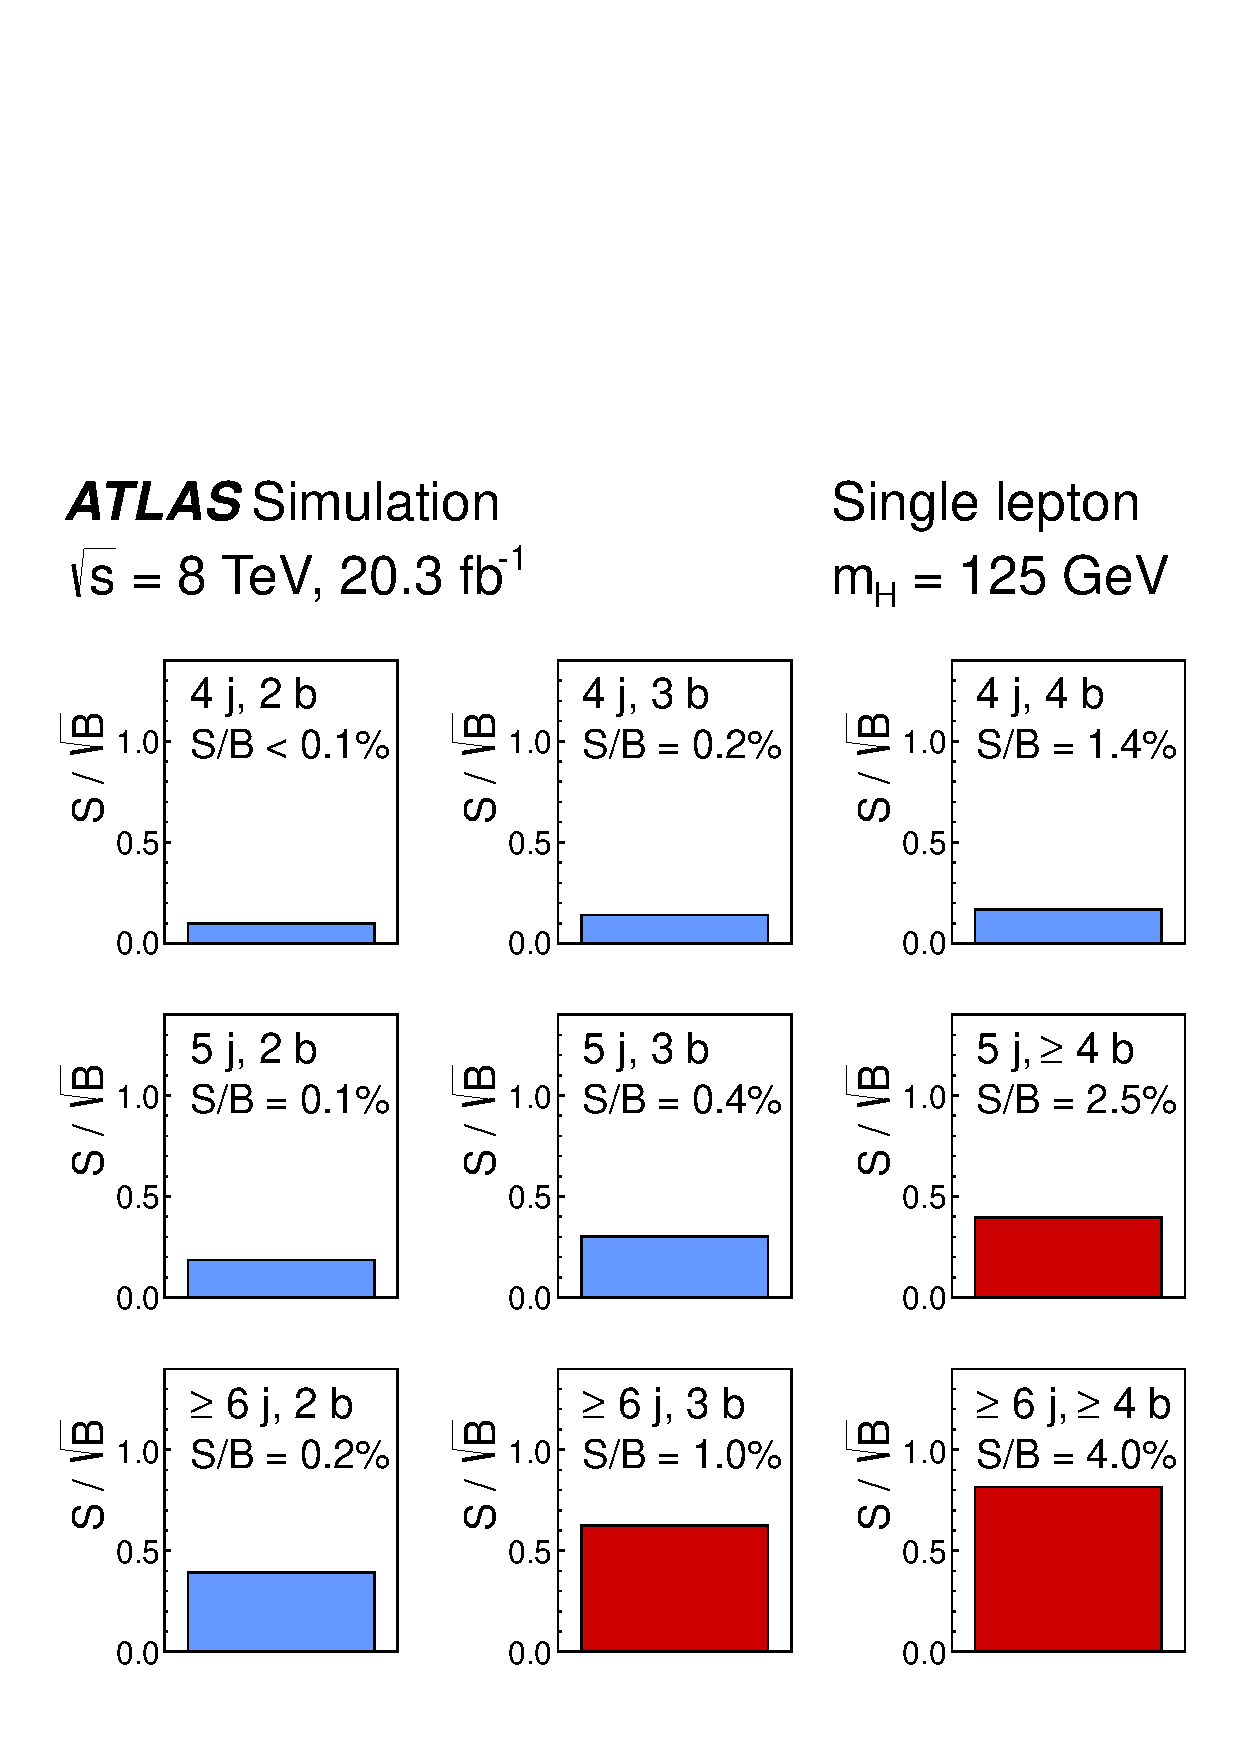
\includegraphics[width=0.7\textwidth]{Analysis/Figures_ttH/soverb}
\caption{$S/\sqrt{B}$ ratio for each of the regions 
assuming SM \xsecs\ and
branching fractions, and $\mH=125\gev$. Each row shows the plots for a
specific jet multiplicity (4, 5, $\geq$6), and the columns show the
$b$-jet multiplicity (2, 3, $\geq$4). Signal-rich regions  
are shaded in dark red, while the rest are shown in light blue. 
The $S/B$ ratio for each region is also noted. 
}
  \label{fig:soverb}
\end{figure}

Figure~\ref{fig:soverb} shows the expected $S/\sqrt{B}$ per analysis region, with the signal-rich regions highlighted in red. Three different NNs are trained in the most sensitive regions: \fivefour, \sixthree\ and \sixfour, to discriminate the \ttH\ signal from the background.
A fourth NN is trained in the \fivethree\ region, to 
separate the two most relevant backgrounds to the analysis: \ttbar+light-jets and \ttHF\ production.
This NN is useful to gain further precision in the measurement of the \ttHF\ background.

The rest of the regions considered in the analysis have a very low
sensitivity and the variable of choice is $\hthad$, defined as the scalar sum of jet \pt.
This variable is chosen due to its sensitivity to the background modeling and to systematic uncertainties such as jet energy scale or $b$-tagging, which have a clear \pt\ dependence.
The signal-depleted regions have high data statistics and the fit of $\hthad$ allows controlling the impact of systematic uncertainties primarily affecting \ttbar+light-jets events.

Figures~\ref{fig:prefit_ttH_1} and~\ref{fig:prefit_ttH_2} show the comparison of data and prediction for the $\hthad$ and NN distributions in each of the analysis
channels considered. The corresponding predicted and observed yields per channel can be found in table~\ref{tab:Prefit_EventsTable_lj}.

\begin{figure}[tpb!]
  \centering
  \begin{subfigure}{0.44\textwidth}
  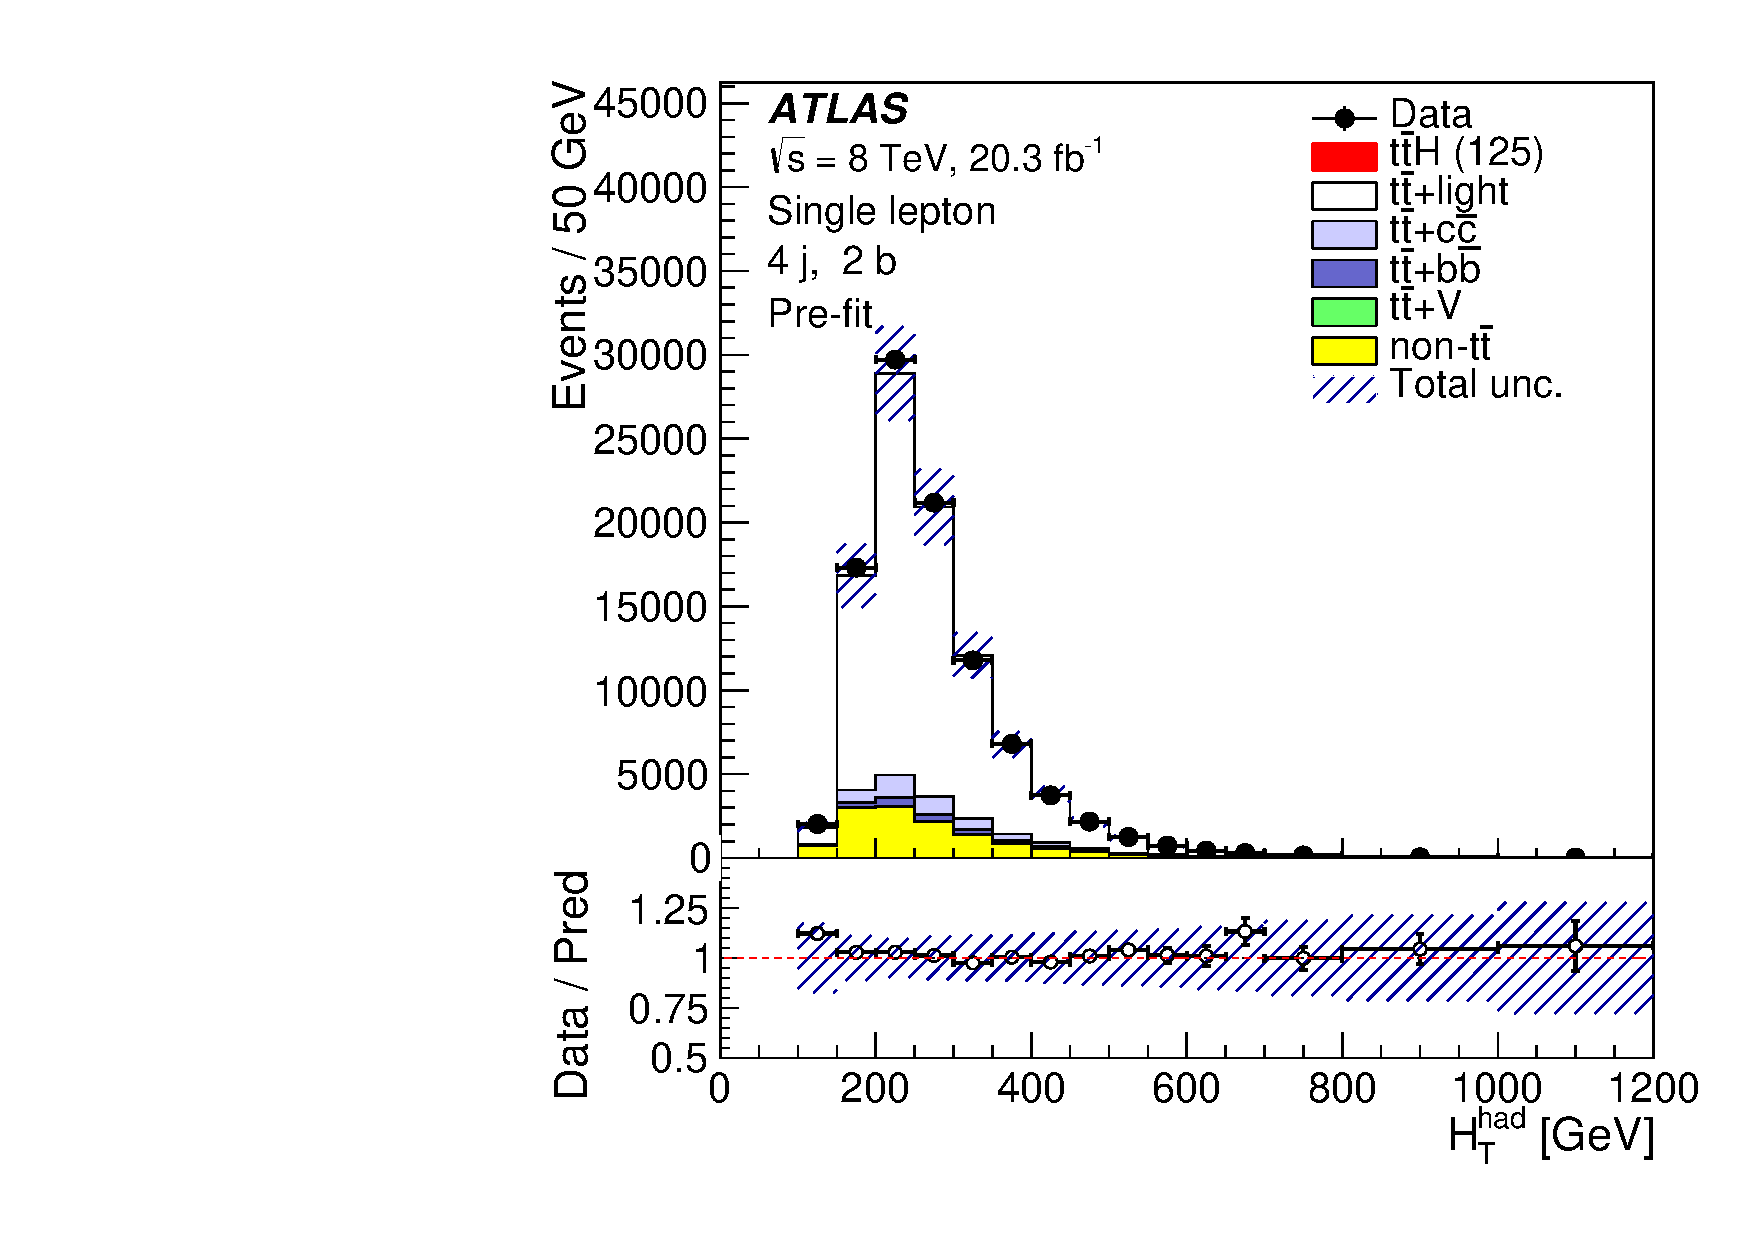
\includegraphics[width=\textwidth]{Analysis/Figures_ttH/HTHad_4jetex2btagex8TeV_before.pdf}
  \caption{}\end{subfigure}
  \begin{subfigure}{0.44\textwidth}
  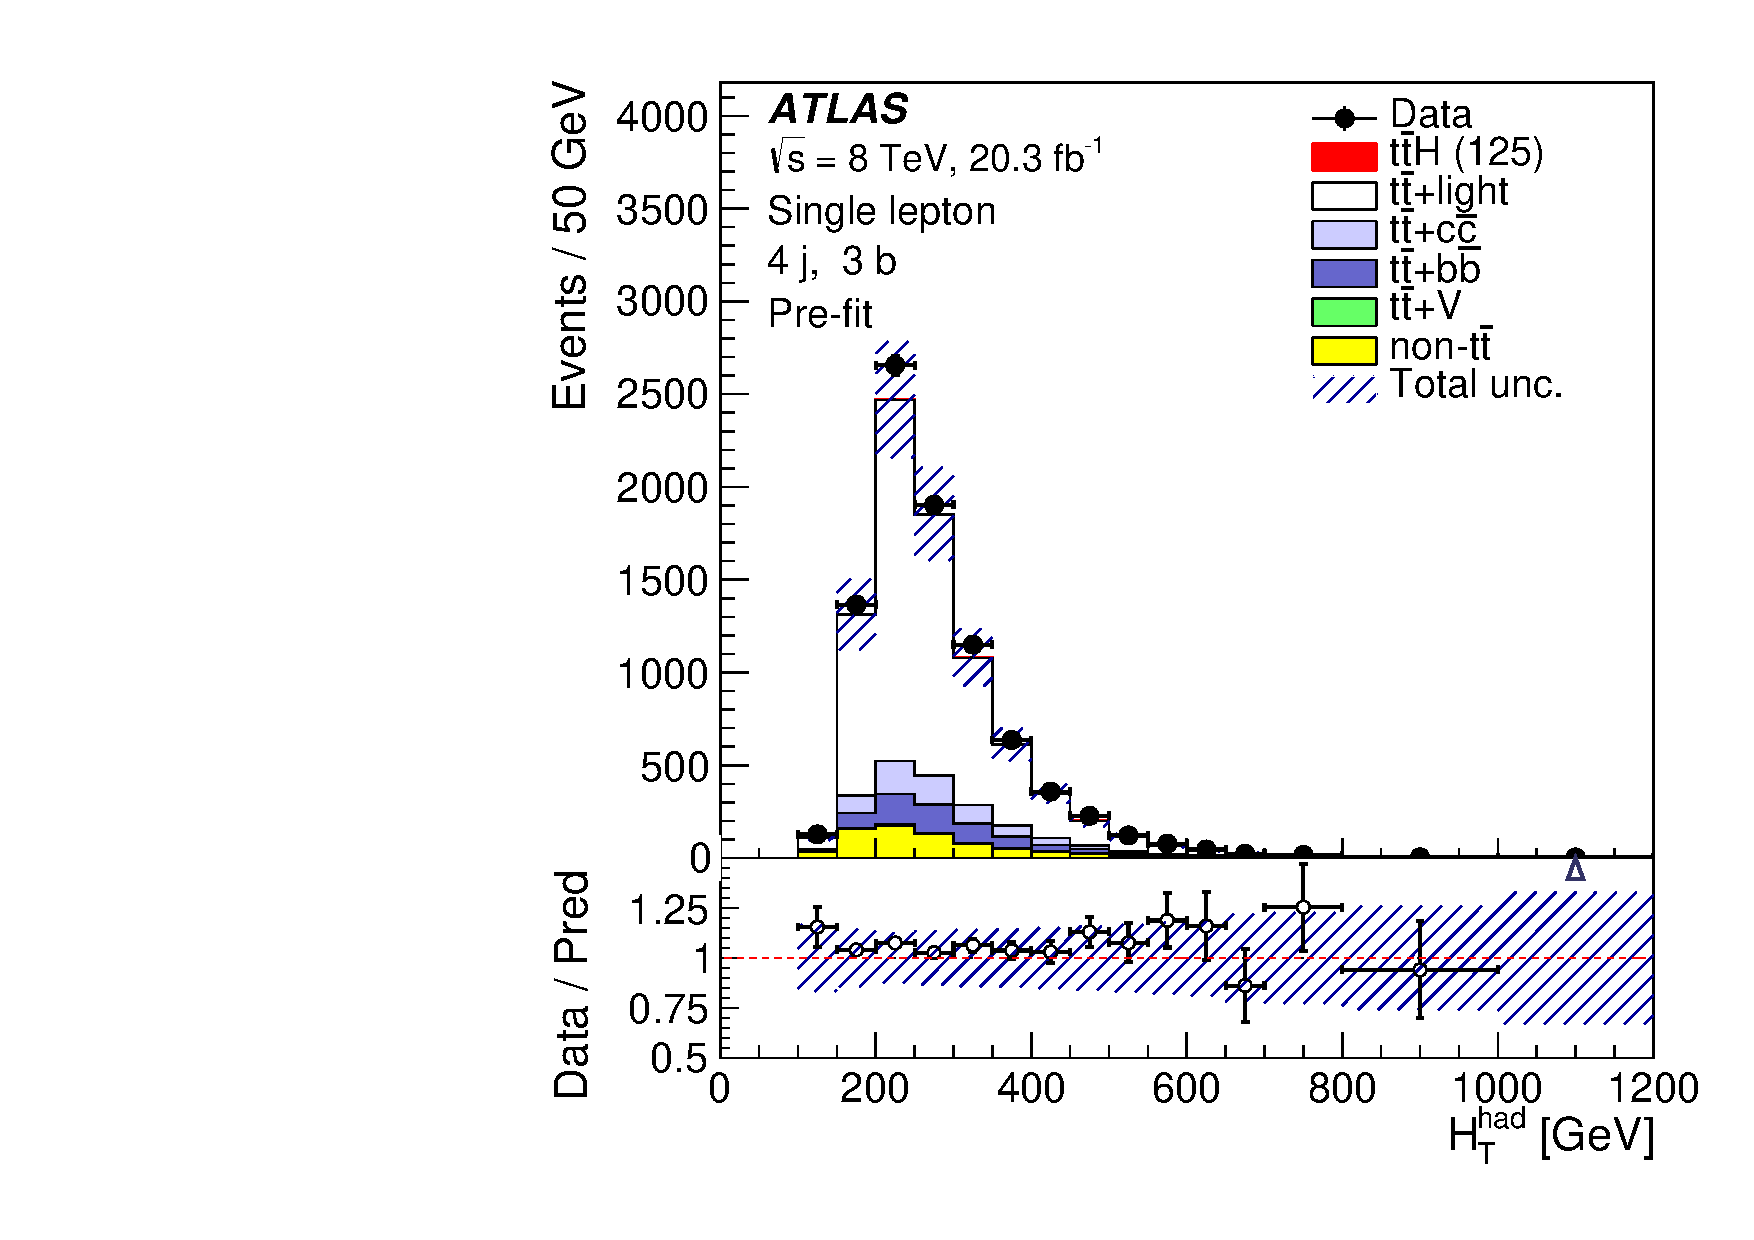
\includegraphics[width=\textwidth]{Analysis/Figures_ttH/HTHad_4jetex3btagex8TeV_before.pdf}
  \caption{}\end{subfigure}
  \begin{subfigure}{0.44\textwidth}
  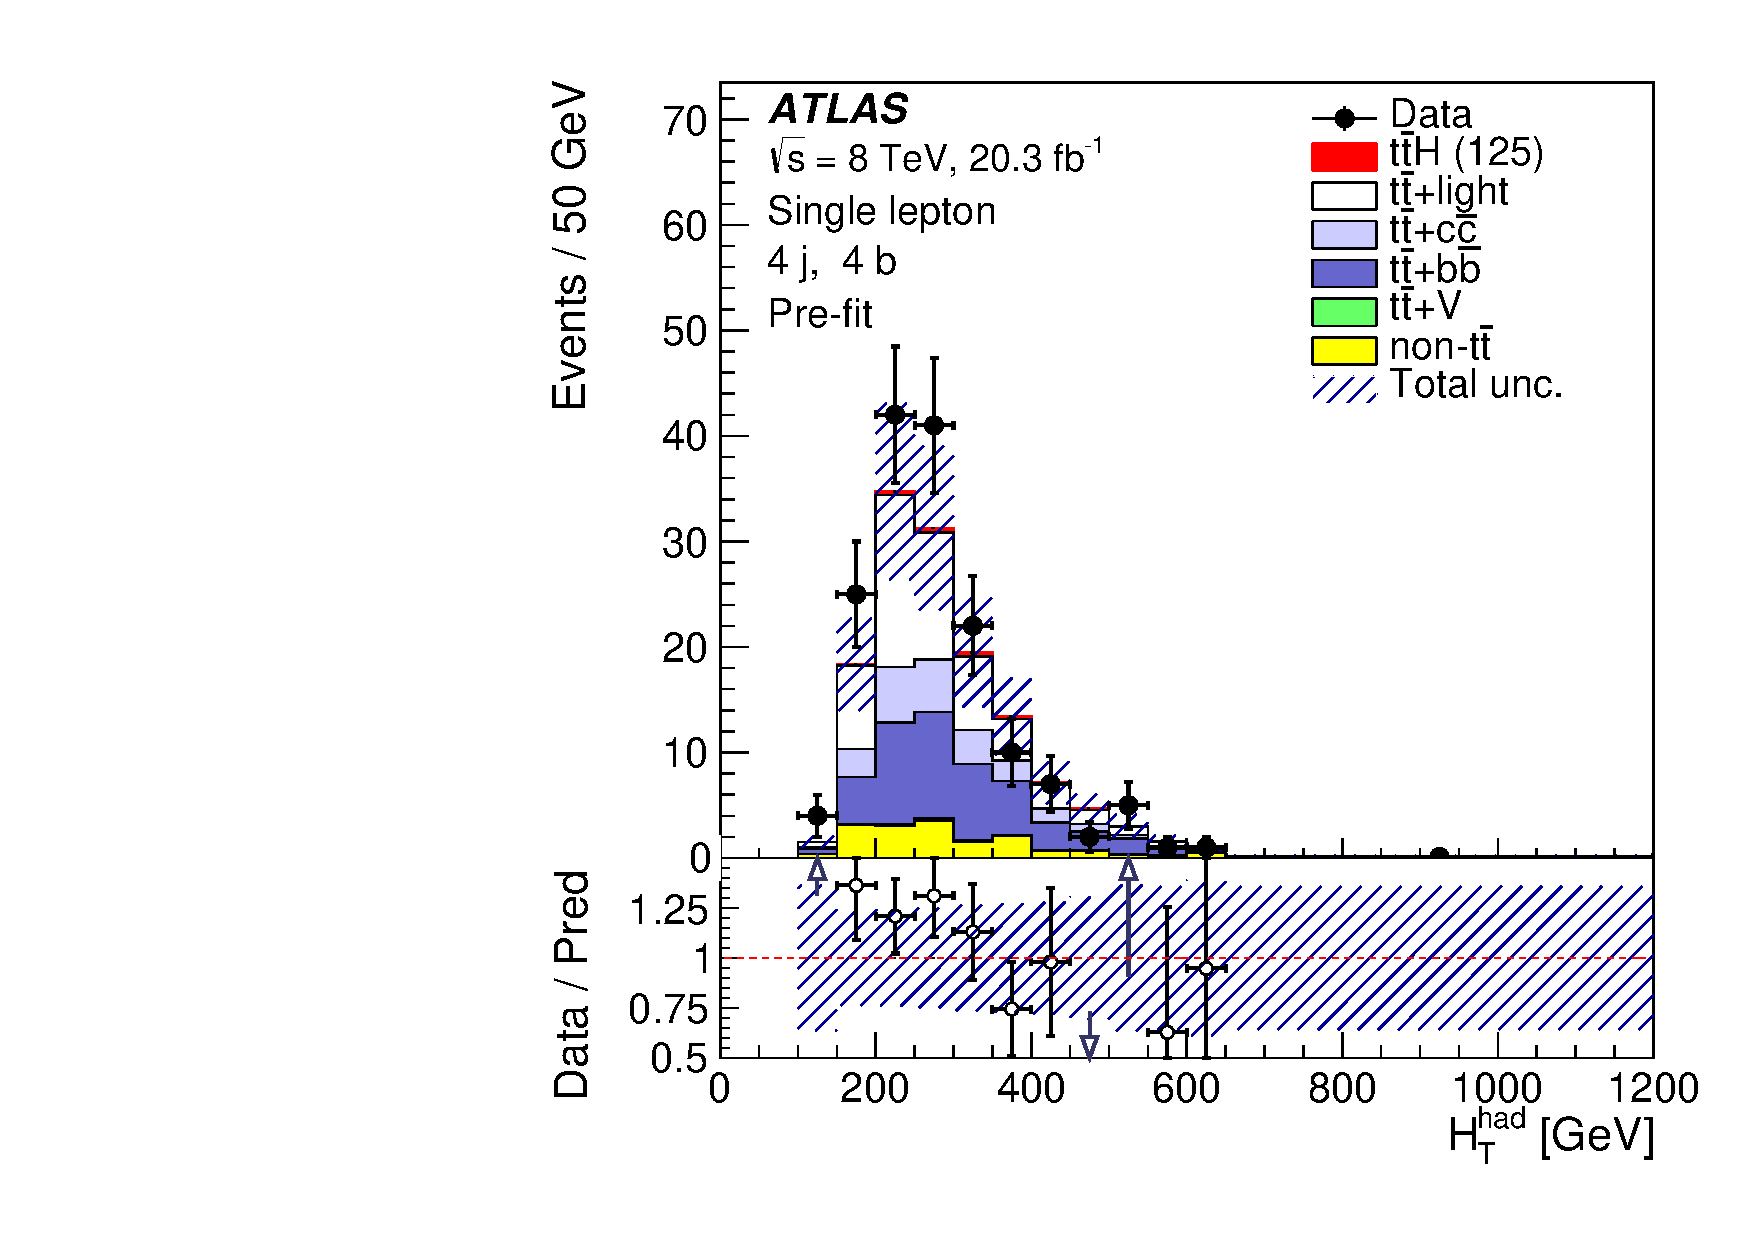
\includegraphics[width=\textwidth]{Analysis/Figures_ttH/HTHad_4jetex4btagin8TeV_before.pdf}
  \caption{}\end{subfigure}
  \begin{subfigure}{0.44\textwidth}
  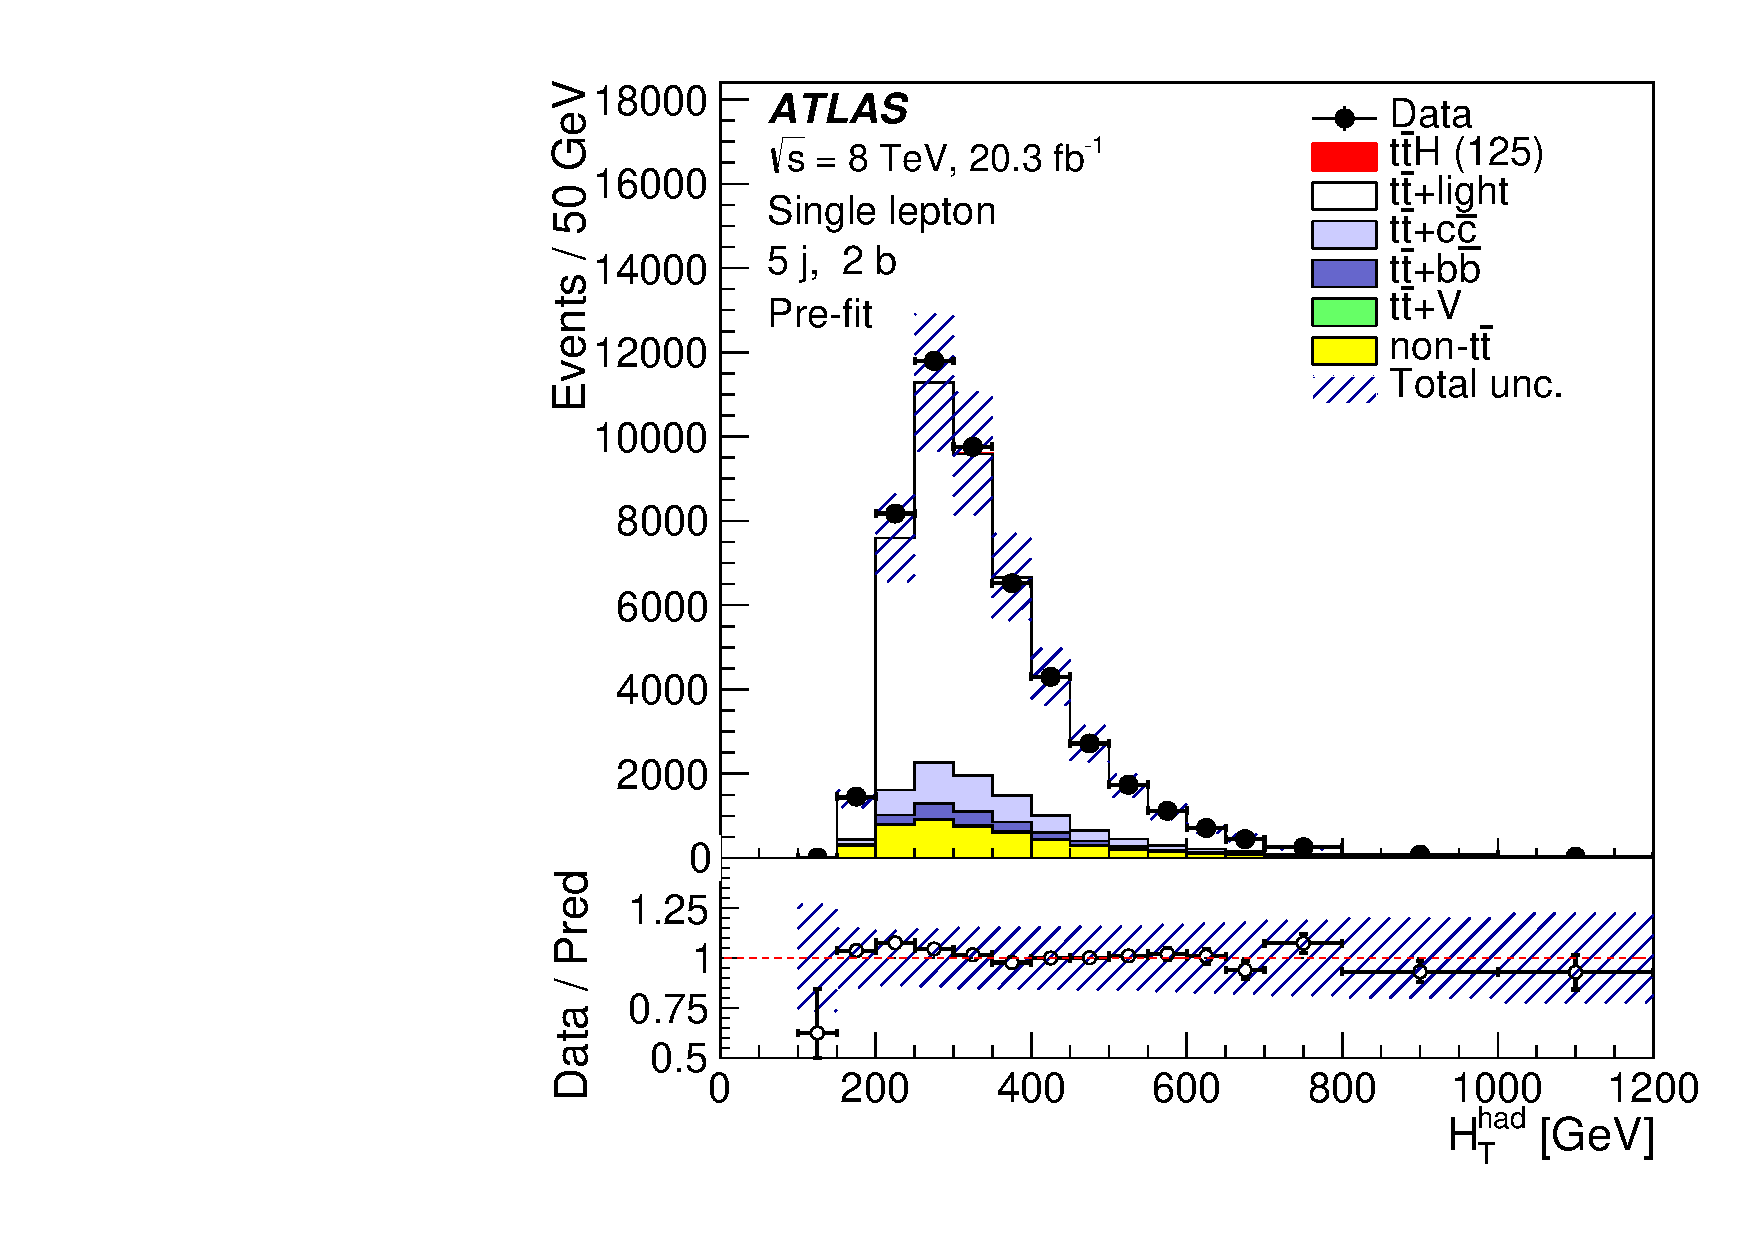
\includegraphics[width=\textwidth]{Analysis/Figures_ttH/HTHad_5jetex2btagex8TeV_before.pdf}
  \caption{}\end{subfigure}
  \begin{subfigure}{0.44\textwidth}
  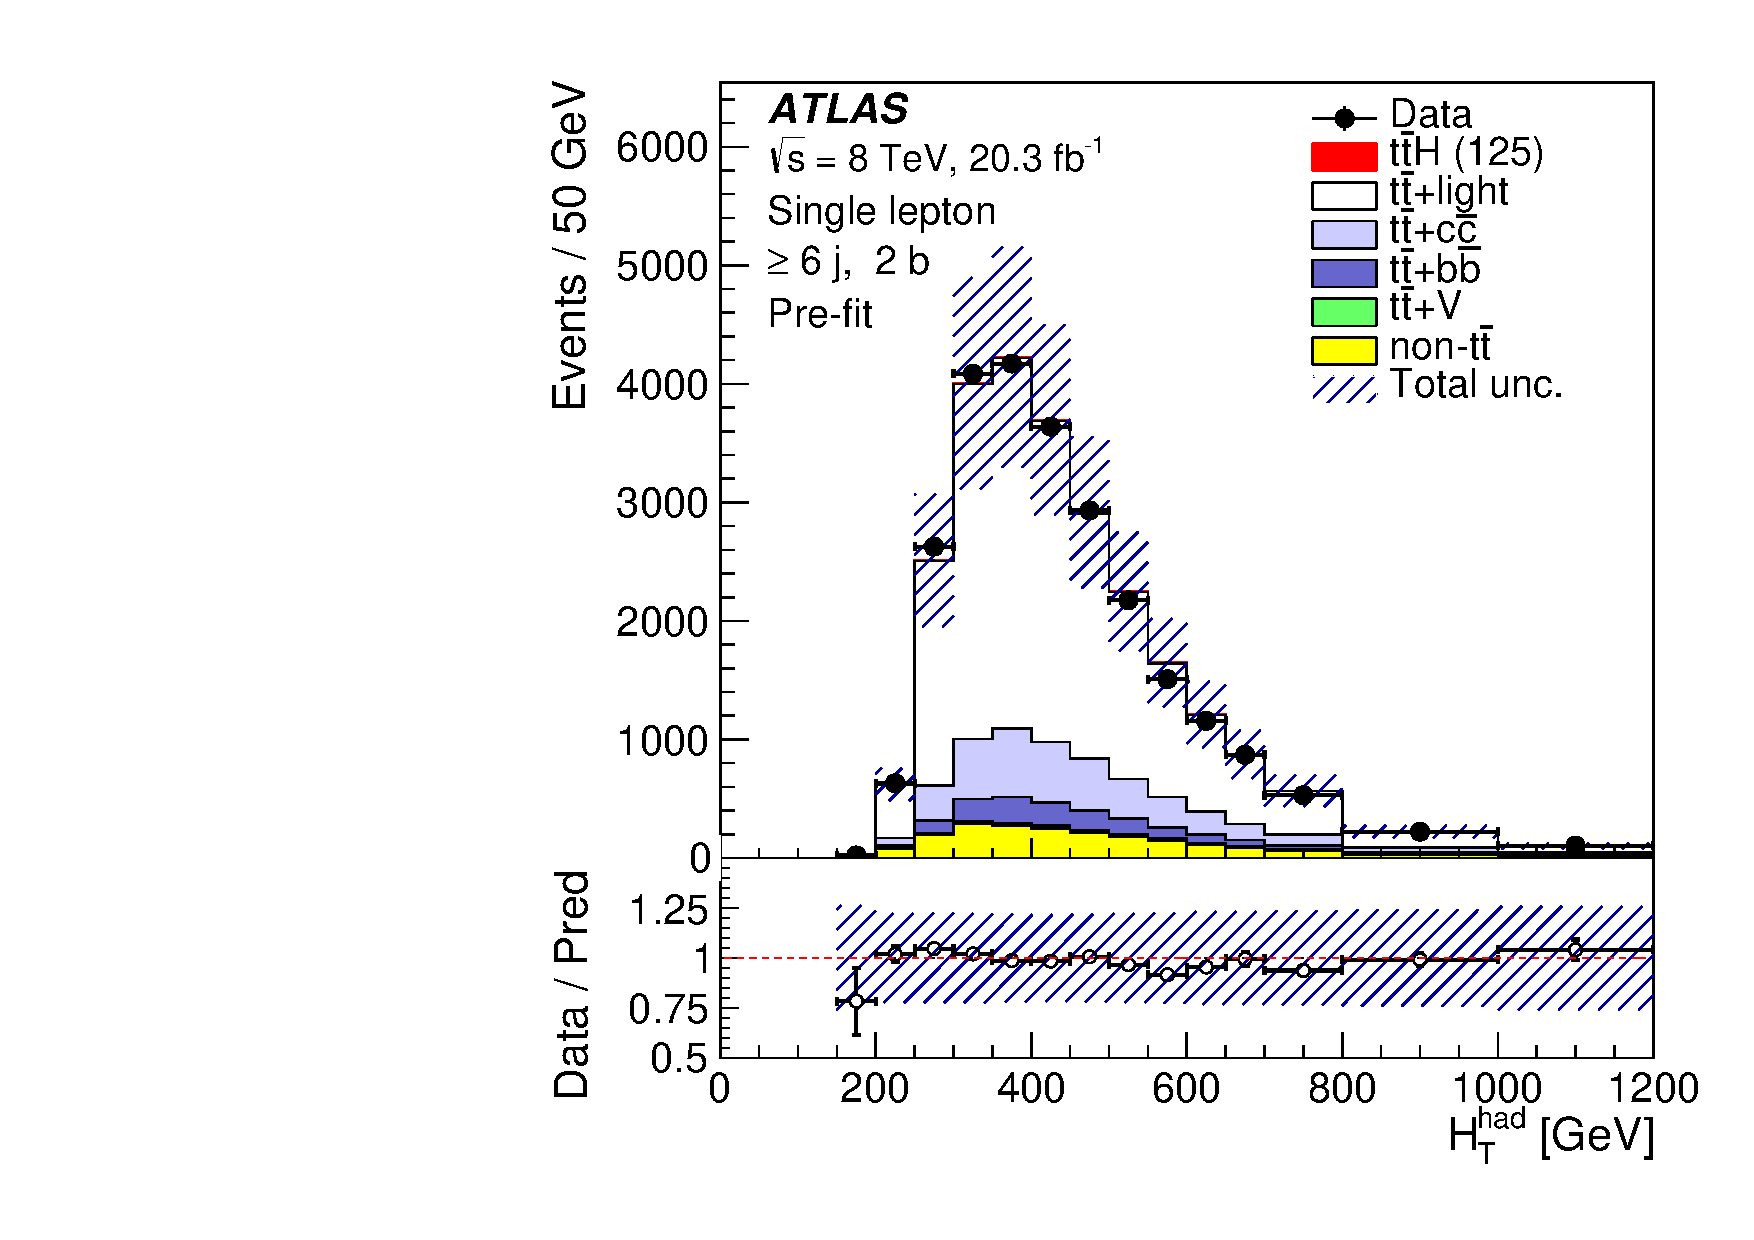
\includegraphics[width=\textwidth]{Analysis/Figures_ttH/HTHad_6jetin2btagex8TeV_before.pdf}
  \caption{}\end{subfigure}
  \caption{Comparison between data and prediction for the $\hthad$ distribution in the signal-depleted regions before the fit:
  (a) \fourtwo, (b) \fourthree, (c) \fourfour, (d) \fivetwo\ and (e) \sixtwo.
  The \tth\ signal is displayed normalized to the SM \xsec\ and stacked on top of the background prediction.
The hashed area represents the uncertainty on the background and the last bin in all figures contains the overflow. 
}
  \label{fig:prefit_ttH_1}
\end{figure}

\begin{figure}[tpb!]
  \centering
  \begin{subfigure}{0.49\textwidth}
  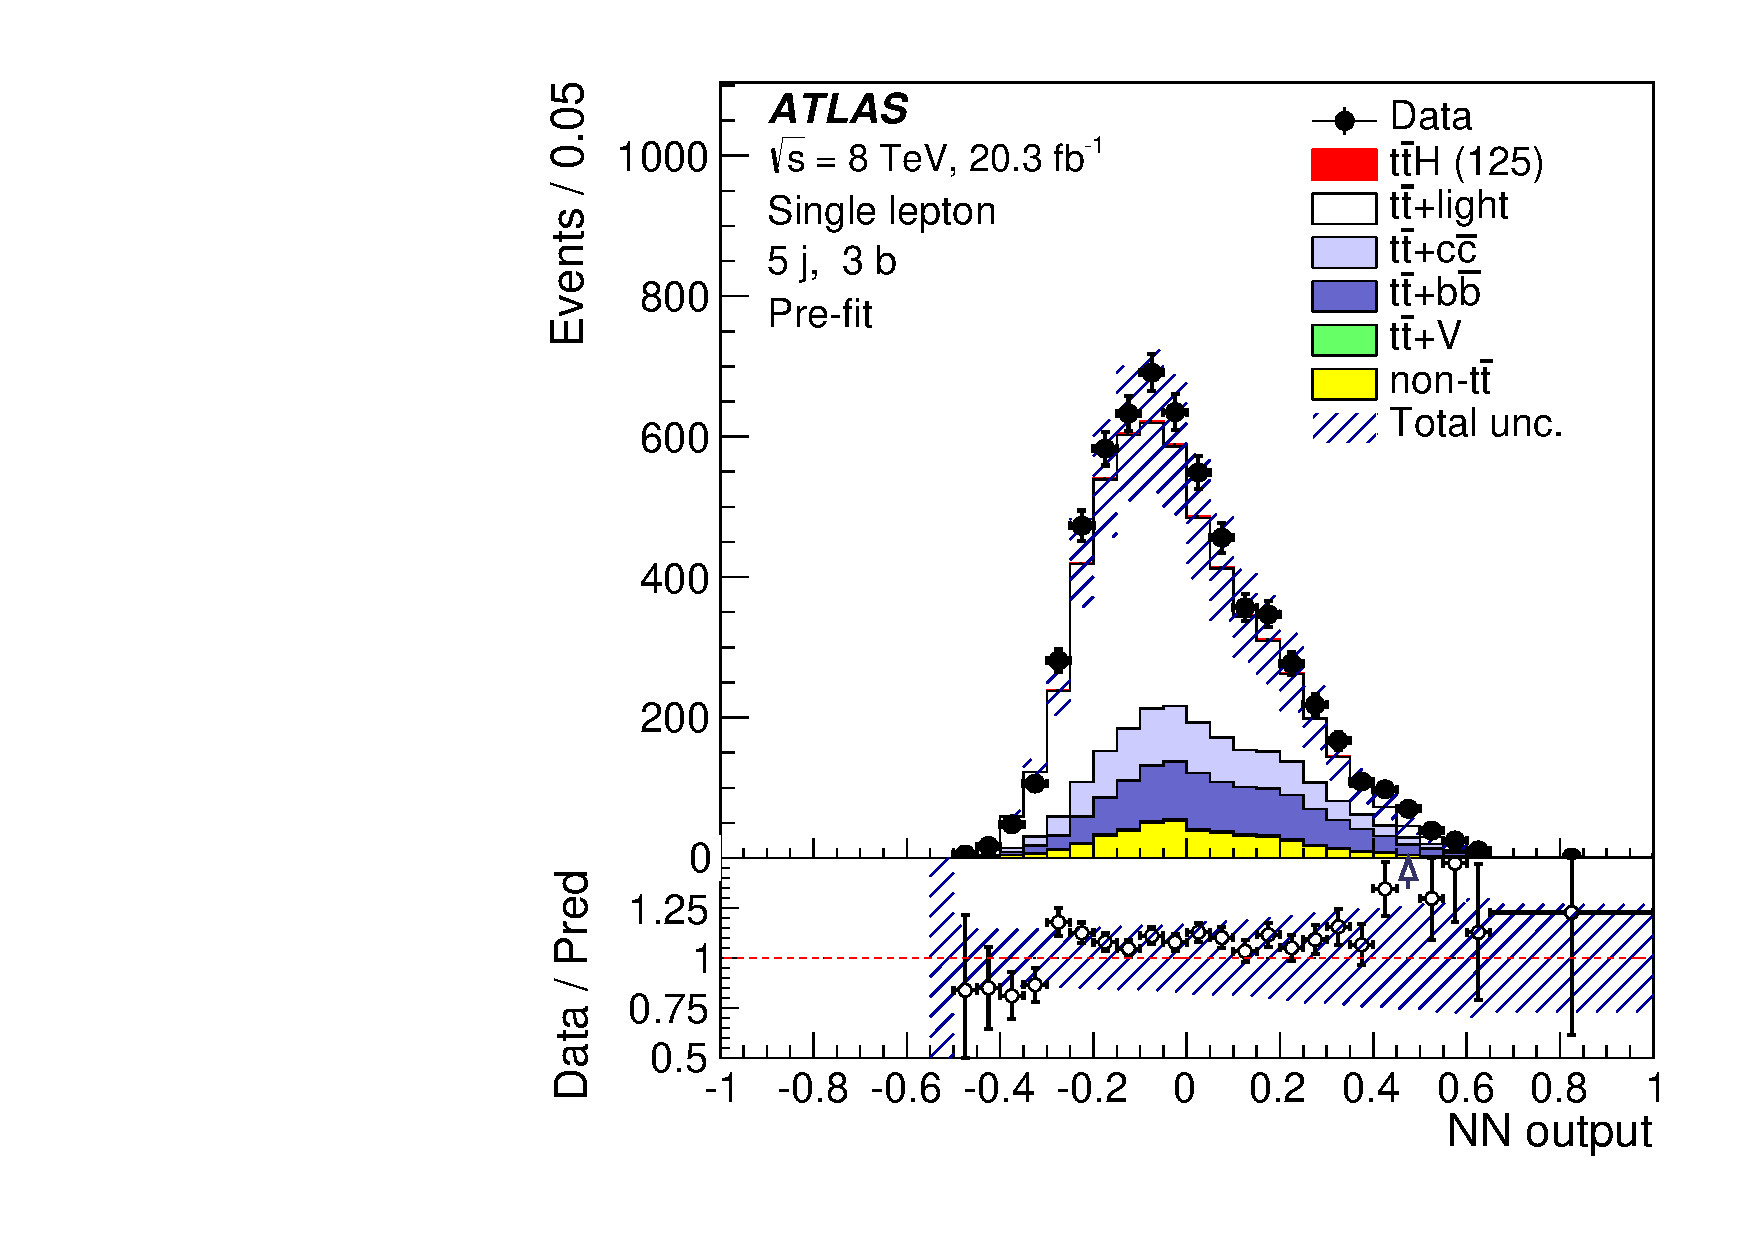
\includegraphics[width=\textwidth]{Analysis/Figures_ttH/NN_5jetex3btagex8TeV_before.pdf}
  \caption{}\end{subfigure}
  \begin{subfigure}{0.49\textwidth}
  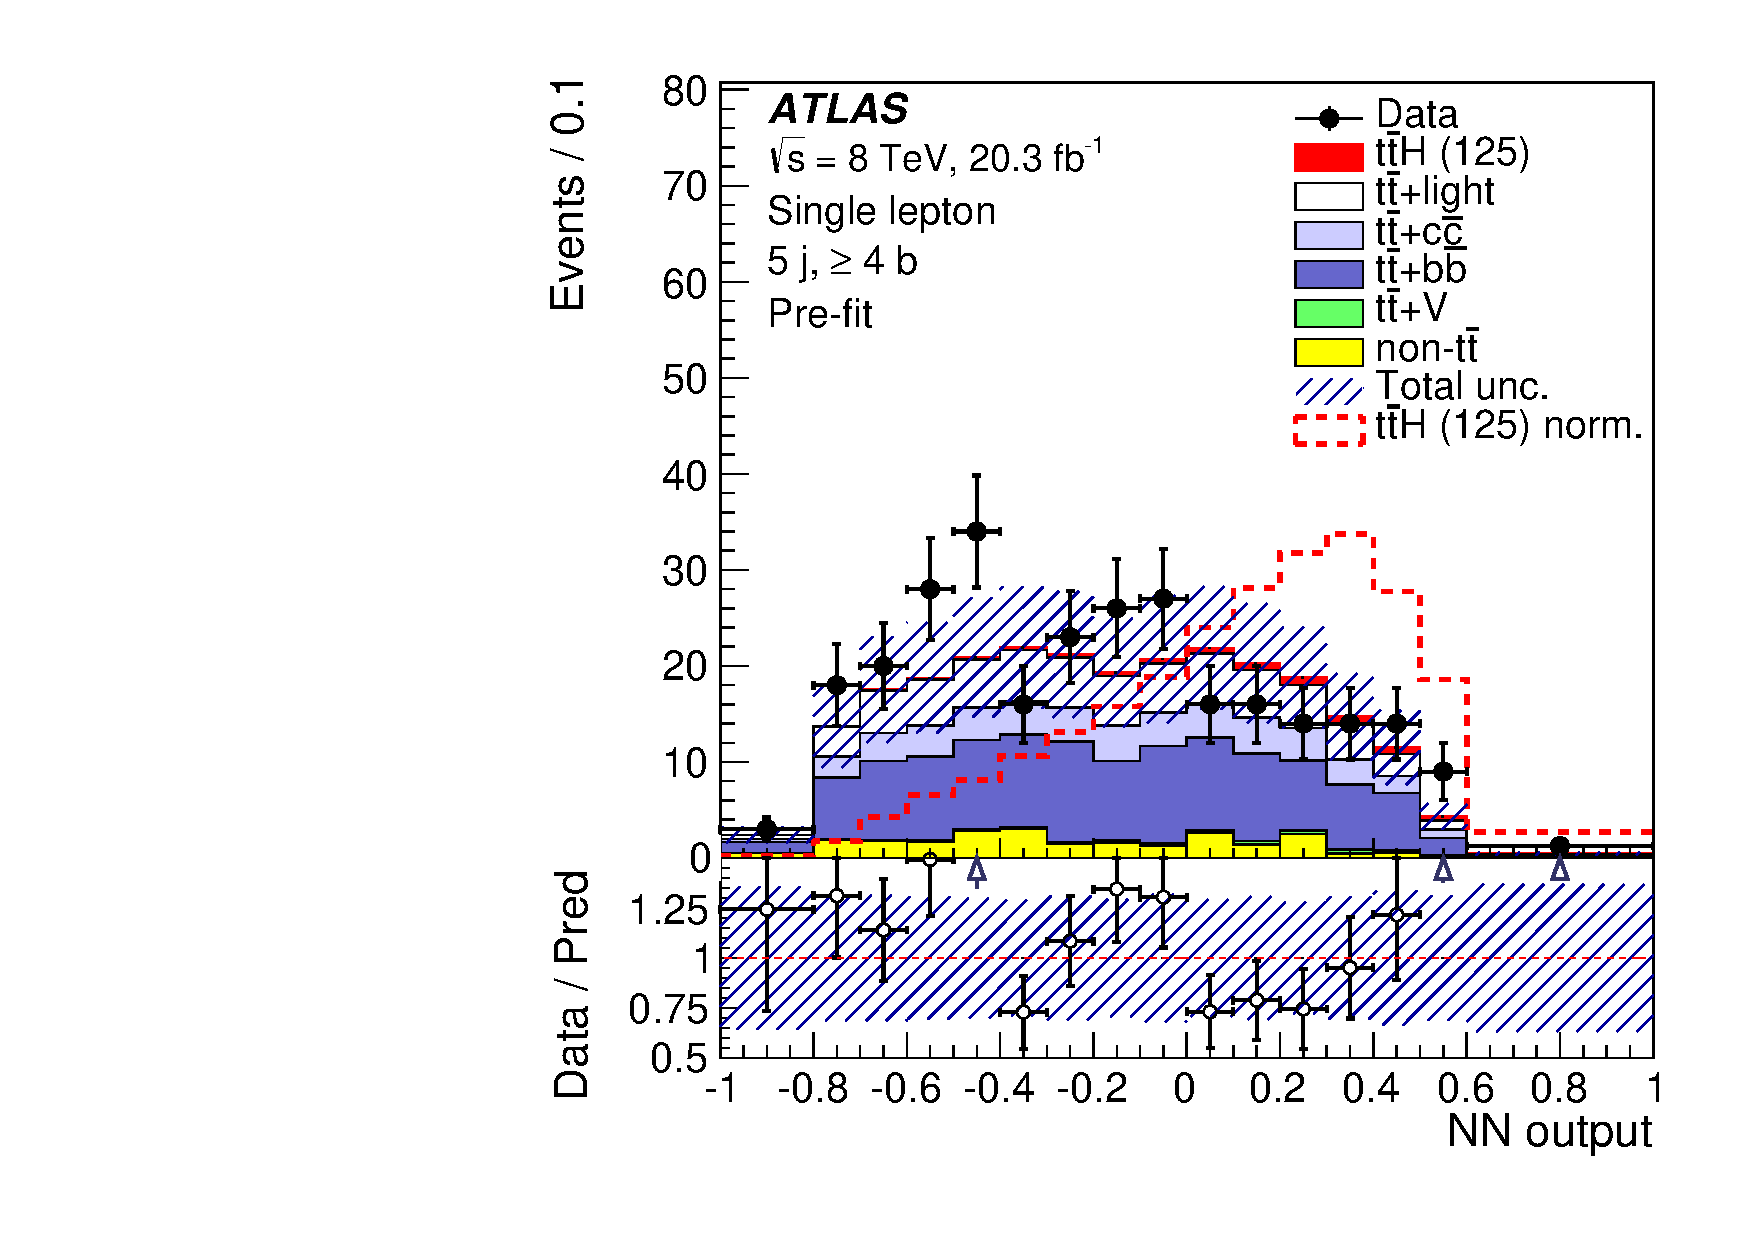
\includegraphics[width=\textwidth]{Analysis/Figures_ttH/NN_5jetex4btagin8TeV_before.pdf}
  \caption{}\end{subfigure}
  \begin{subfigure}{0.49\textwidth}
  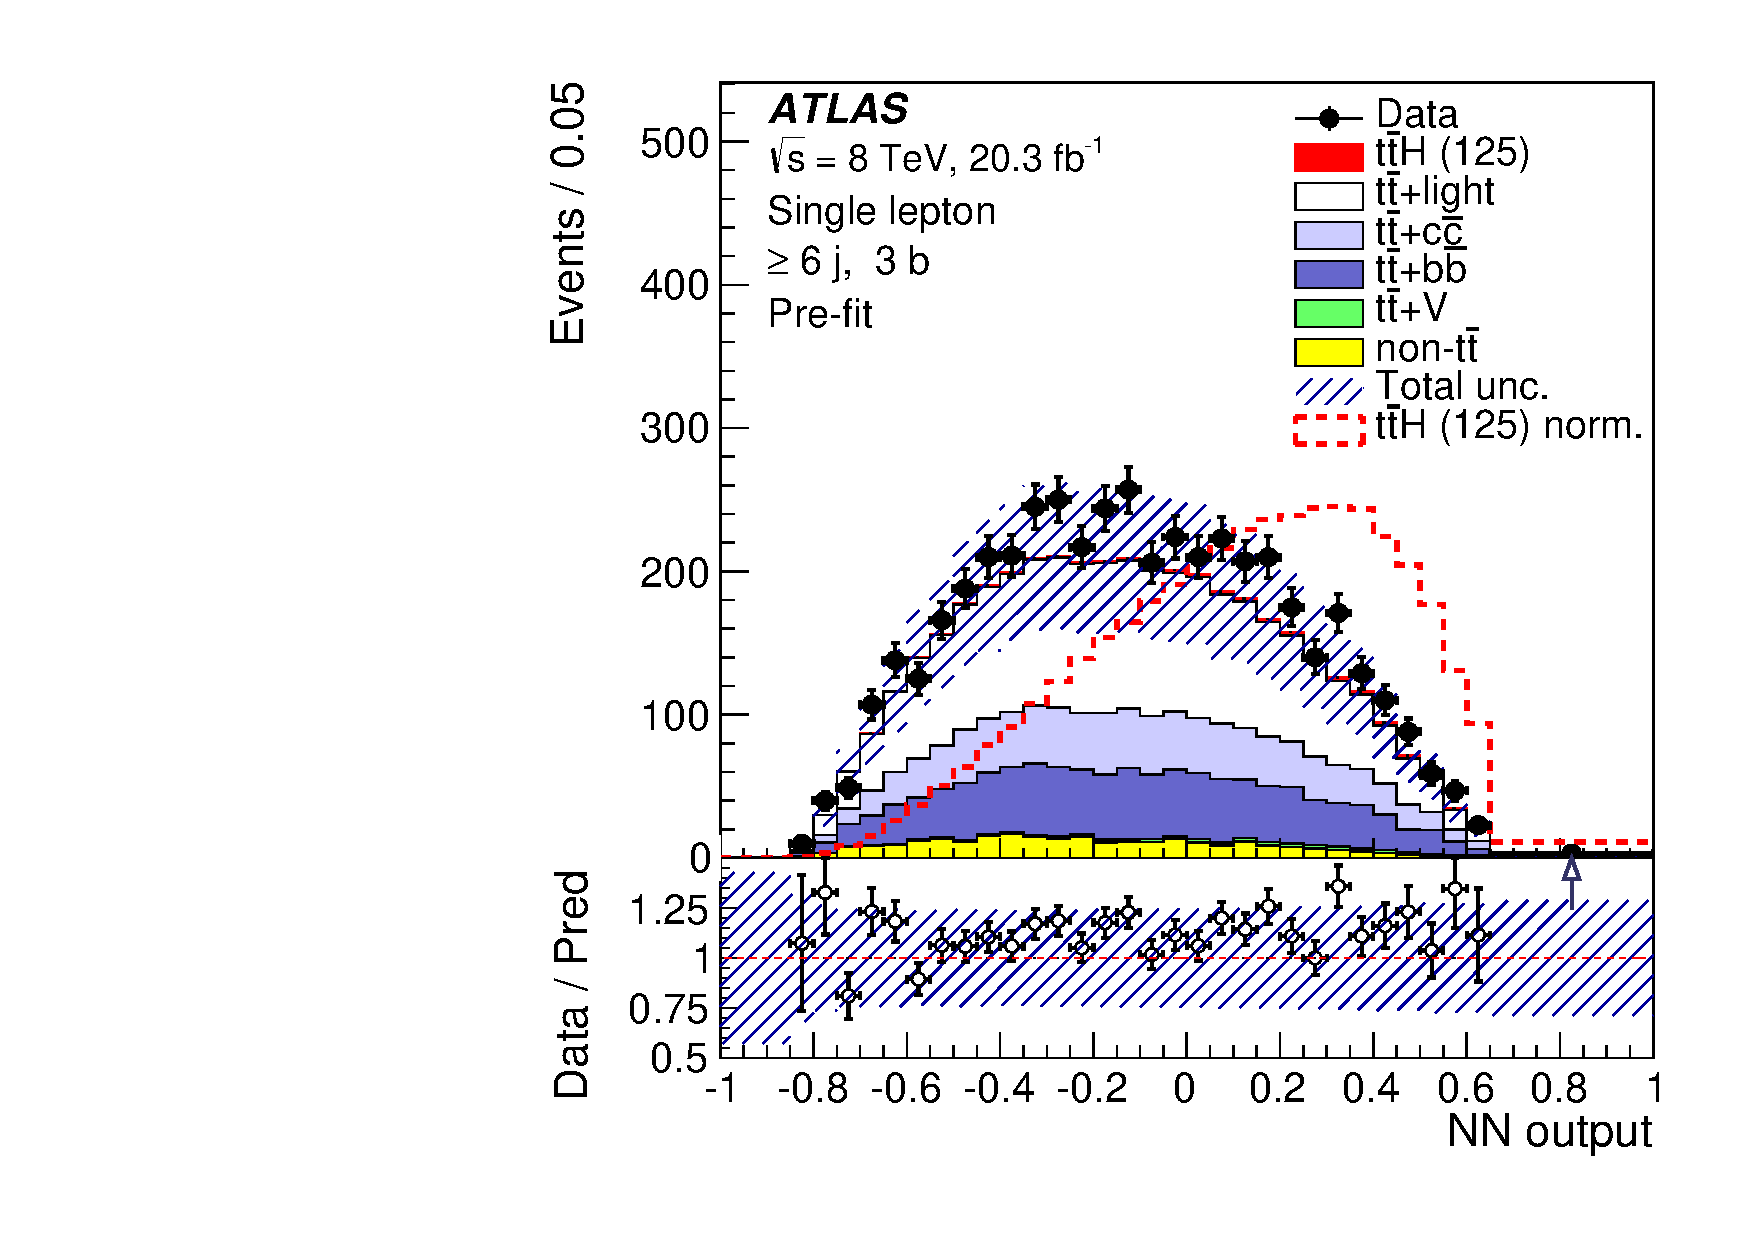
\includegraphics[width=\textwidth]{Analysis/Figures_ttH/NN_6jetin3btagex8TeV_before.pdf}
  \caption{}\end{subfigure}
  \begin{subfigure}{0.49\textwidth}
  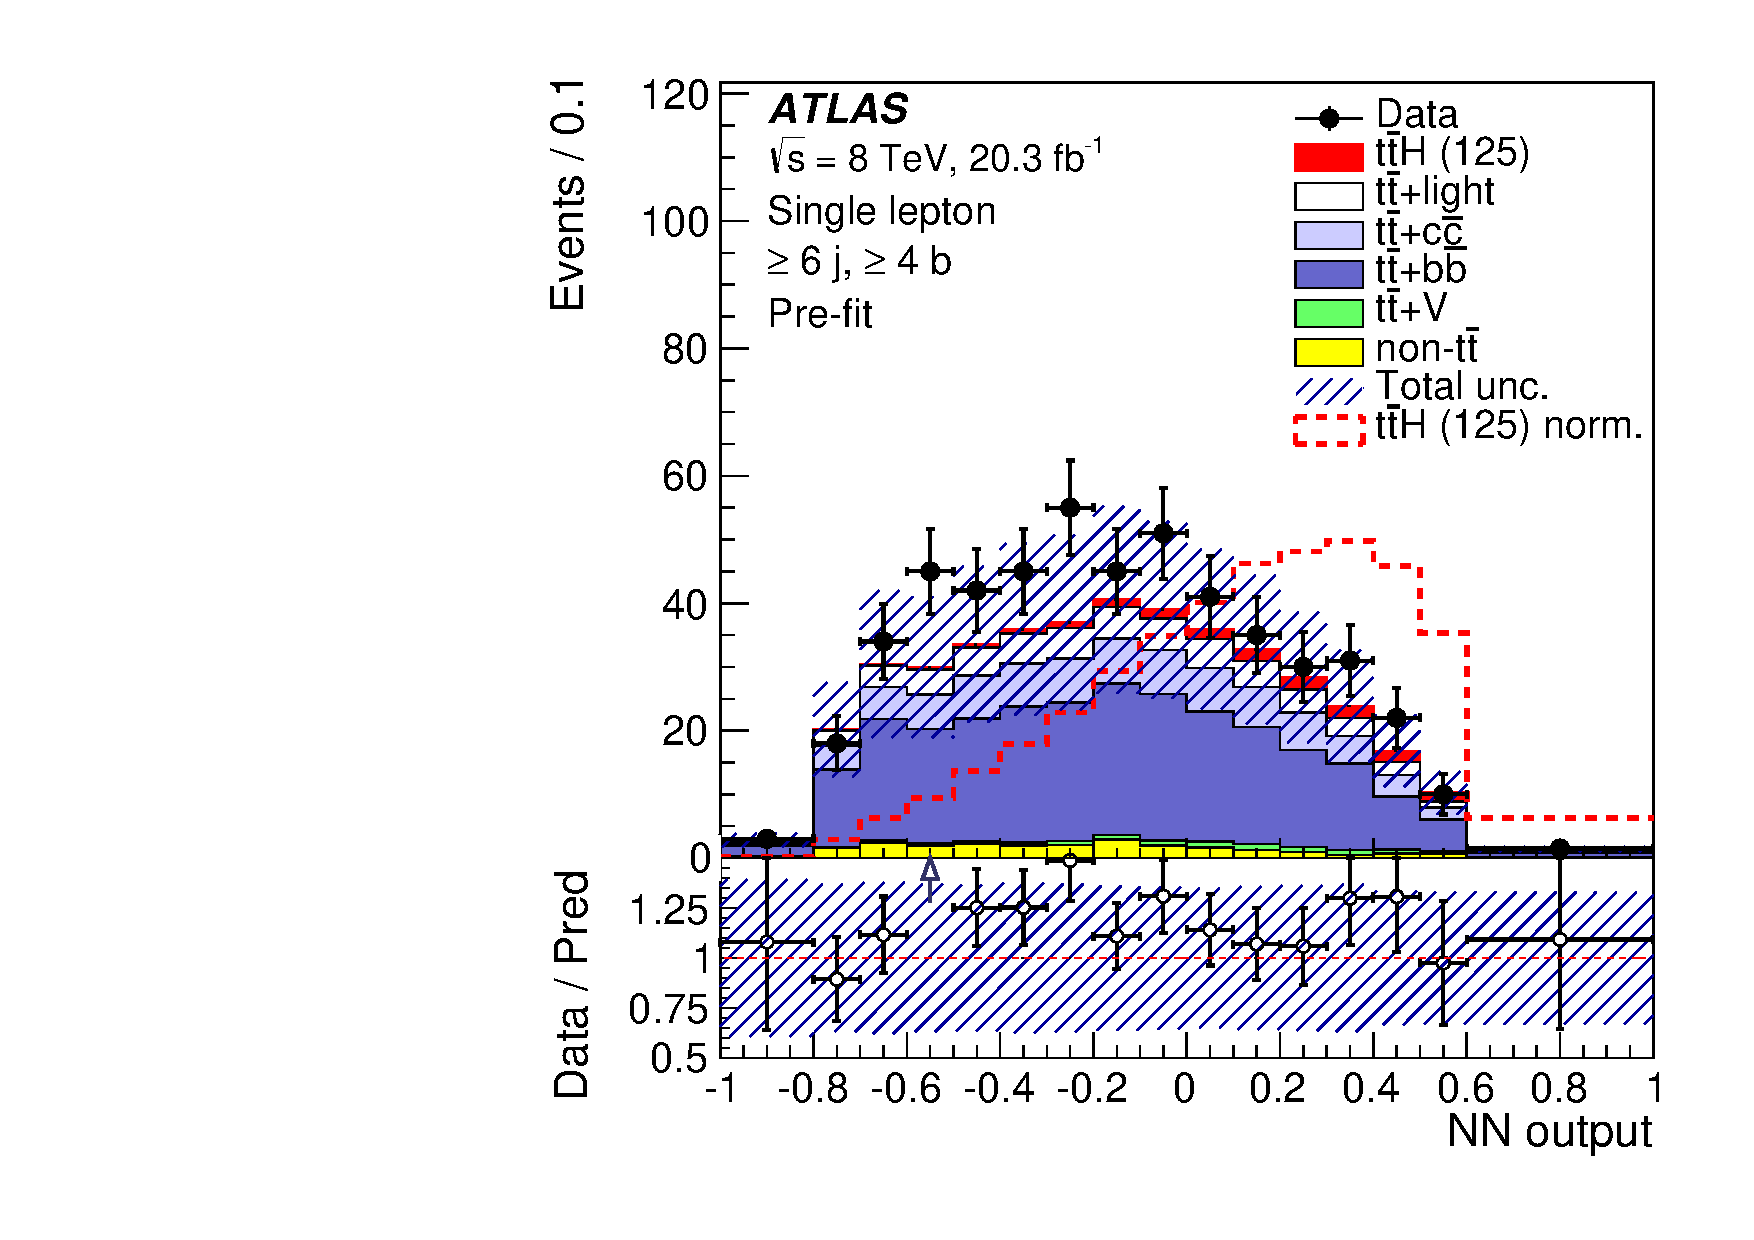
\includegraphics[width=\textwidth]{Analysis/Figures_ttH/NN_6jetin4btagin8TeV_before.pdf}
  \caption{}\end{subfigure}
  \caption{Comparison between data and prediction for the $NN$ distribution in the signal-rich regions and the \fivethree\ region before the fit:
  (a) \fivethree, (b) \fivefour, (c) \sixthree\ and (d) \sixfour.
  The \tth\ signal is displayed normalized to the SM \xsec\ (solid) and normalized to the total background prediction (hashed line) in order to compare the shape of the distributions.
The hashed area represents the uncertainty on the background and the last bin in all figures contains the overflow. 
}
  \label{fig:prefit_ttH_2}
\end{figure}


\begin{table}[tp!]
\begin{center}
\begin{tabular}{l*{3}{r@{$\,\pm\,$}r}}%
\hline\hline
 & \multicolumn{2}{c}{4 j, 2 b} & \multicolumn{2}{c}{4 j, 3 b} & \multicolumn{2}{c}{4 j, 4 b}\\
\hline
$t\bar{t}H$ (125) & \numRF{30.66}{2} & \numRF{2.83}{1} & \numRF{12.85}{2} & \numRF{1.50}{1} & \numRF{1.95}{2} & \numRF{0.29}{1}\\
$t\bar{t}+$ light & \numRF{76659.58}{2} & \numRF{7528.04}{2} & \numRF{6165.66}{2} & \numRF{745.14}{2} & \numRF{53.15}{2} & \numRF{12.13}{2}\\
$t\bar{t}+c\bar{c}$ & \numRF{4868.29}{2} & \numRF{2964.75}{2} & \numRF{682.12}{2} & \numRF{390.52}{2} & \numRF{21.21}{2} & \numRF{11.95}{2}\\
$t\bar{t}+b\bar{b}$ & \numRF{1844.41}{2} & \numRF{1071.64}{2} & \numRF{679.72}{2} & \numRF{378.59}{2} & \numRF{44.24}{2} & \numRF{24.75}{2}\\
$W$+jets & \numRF{5118.04}{2} & \numRF{2981.90}{2} & \numRF{224.65}{2} & \numRF{133.00}{2} & \numRF{5.52}{2} & \numRF{3.31}{2}\\
$Z$+jets & \numRF{1125.82}{2} & \numRF{597.54}{2} & \numRF{50.23}{2} & \numRF{27.25}{2} & \numRF{0.90}{1} & \numRF{0.56}{1}\\
Single top & \numRF{4932.12}{2} & \numRF{644.49}{2} & \numRF{337.36}{2} & \numRF{60.37}{2} & \numRF{6.78}{2} & \numRF{1.58}{2}\\
Diboson & \numRF{216.76}{2} & \numRF{70.50}{2} & \numRF{11.49}{2} & \numRF{4.06}{2} & \numRF{0.24}{1} & \numRF{0.12}{1}\\
$t\bar{t}+V$ & \numRF{122.18}{2} & \numRF{40.45}{2} & \numRF{15.46}{2} & \numRF{5.10}{2} & \numRF{0.89}{1} & \numRF{0.30}{1}\\
Multijet & \numRF{1564.61}{2} & \numRF{619.84}{2} & \numRF{102.21}{2} & \numRF{37.13}{2} & \numRF{3.52}{2} & \numRF{1.28}{2}\\
\hline
Total & \numRF{96482.46}{2} & \numRF{9509.42}{2}   & \numRF{8281.77}{2} & \numRF{1073.67}{2}   & \numRF{138.40}{2} & \numRF{33.85}{2}  \\
\hline
Data & \multicolumn{2}{l}{\num{98049}}  & \multicolumn{2}{l}{\num{8752}}  & \multicolumn{2}{l}{\num{161}} \\
\hline\hline     \\
\end{tabular}
%%\\
\vspace{0.1cm}

\begin{tabular}{l*{3}{r@{$\,\pm\,$}r}}%
\hline\hline
 & \multicolumn{2}{c}{5 j, 2 b} & \multicolumn{2}{c}{5 j, 3 b} & \multicolumn{2}{c}{5 j, $\geq$ 4 b}\\
\hline
$t\bar{t}H$ (125) & \numRF{40.86}{2} & \numRF{2.05}{1} & \numRF{22.65}{2} & \numRF{1.77}{1} & \numRF{6.22}{2} & \numRF{0.80}{1}\\
$t\bar{t}+$ light & \numRF{37606.38}{2} & \numRF{5512.23}{2} & \numRF{3484.78}{2} & \numRF{524.44}{2} & \numRF{60.84}{2} & \numRF{14.73}{2}\\
$t\bar{t}+c\bar{c}$ & \numRF{4298.98}{2} & \numRF{2380.58}{2} & \numRF{809.59}{2} & \numRF{455.46}{2} & \numRF{42.80}{2} & \numRF{24.68}{2}\\
$t\bar{t}+b\bar{b}$ & \numRF{1665.02}{2} & \numRF{876.06}{2} & \numRF{886.03}{2} & \numRF{477.26}{2} & \numRF{114.90}{2} & \numRF{63.25}{2}\\
$W$+jets & \numRF{1938.28}{2} & \numRF{1232.45}{2} & \numRF{135.32}{2} & \numRF{86.95}{2} & \numRF{5.89}{2} & \numRF{3.85}{2}\\
$Z$+jets & \numRF{405.34}{2} & \numRF{237.67}{2} & \numRF{28.91}{2} & \numRF{17.07}{2} & \numRF{1.47}{2} & \numRF{0.90}{1}\\
Single top & \numRF{1880.73}{2} & \numRF{364.26}{2} & \numRF{194.65}{2} & \numRF{41.44}{2} & \numRF{8.32}{2} & \numRF{1.32}{2}\\
Diboson & \numRF{96.52}{2} & \numRF{38.51}{2} & \numRF{8.02}{2} & \numRF{3.43}{2} & \numRF{0.40}{1} & \numRF{0.20}{1}\\
$t\bar{t}+V$ & \numRF{145.41}{2} & \numRF{47.67}{2} & \numRF{26.47}{2} & \numRF{8.58}{1} & \numRF{3.10}{2} & \numRF{1.02}{2}\\
Multijet & \numRF{460.79}{2} & \numRF{165.45}{2} & \numRF{69.93}{2} & \numRF{27.57}{2} & \numRF{8.31}{2} & \numRF{3.70}{2}\\
\hline
Total & \numRF{48538.31}{2} & \numRF{6957.37}{2}   & \numRF{5666.35}{2} & \numRF{982.65}{2}   & \numRF{252.25}{2} & \numRF{75.03}{2}  \\
\hline
Data & \multicolumn{2}{l}{\num{49699}}  & \multicolumn{2}{l}{\num{6199}}  & \multicolumn{2}{l}{\num{286}} \\
\hline\hline     \\
\end{tabular}
%%\\
\vspace{0.1cm}

\begin{tabular}{l*{3}{r@{$\,\pm\,$}r}}%
\hline\hline
 & \multicolumn{2}{c}{$\geq$ 6 j, 2 b} & \multicolumn{2}{c}{$\geq$ 6 j, 3 b} & \multicolumn{2}{c}{$\geq$ 6 j, $\geq$ 4 b}\\
\hline
$t\bar{t}H$ (125) & \numRF{63.73}{2} & \numRF{4.99}{1} & \numRF{40.23}{2} & \numRF{3.46}{1} & \numRF{16.49}{2} & \numRF{2.04}{1}\\
$t\bar{t}+$ light & \numRF{18849.67}{2} & \numRF{4402.80}{2} & \numRF{2008.43}{2} & \numRF{463.33}{2} & \numRF{52.40}{2} & \numRF{16.73}{2}\\
$t\bar{t}+c\bar{c}$ & \numRF{3725.70}{2} & \numRF{2086.67}{2} & \numRF{845.95}{2} & \numRF{482.52}{2} & \numRF{79.07}{2} & \numRF{46.46}{2}\\
$t\bar{t}+b\bar{b}$ & \numRF{1424.18}{2} & \numRF{767.00}{2} & \numRF{973.67}{2} & \numRF{526.66}{2} & \numRF{245.44}{2} & \numRF{132.77}{2}\\
$W$+jets & \numRF{911.56}{2} & \numRF{624.38}{2} & \numRF{96.70}{2} & \numRF{66.00}{2} & \numRF{8.60}{2} & \numRF{6.18}{2}\\
$Z$+jets & \numRF{183.25}{2} & \numRF{118.21}{2} & \numRF{19.00}{2} & \numRF{12.44}{2} & \numRF{1.54}{2} & \numRF{1.01}{2}\\
Single top & \numRF{836.37}{2} & \numRF{220.14}{2} & \numRF{121.73}{2} & \numRF{35.35}{2} & \numRF{11.91}{2} & \numRF{3.68}{2}\\
Diboson & \numRF{50.45}{2} & \numRF{24.31}{2} & \numRF{5.98}{2} & \numRF{3.01}{2} & \numRF{0.54}{1} & \numRF{0.27}{1}\\
$t\bar{t}+V$ & \numRF{182.33}{2} & \numRF{59.31}{2} & \numRF{44.58}{2} & \numRF{14.25}{2} & \numRF{8.45}{2} & \numRF{2.77}{2}\\
Multijet & \numRF{181.42}{2} & \numRF{66.00}{2} & \numRF{21.31}{2} & \numRF{7.63}{1} & \numRF{1.09}{2} & \numRF{0.52}{1}\\
\hline
Total & \numRF{26408.66}{2} & \numRF{5760.23}{2}   & \numRF{4177.59}{2} & \numRF{1018.85}{2}   & \numRF{425.53}{2} & \numRF{151.98}{2}  \\
\hline
Data & \multicolumn{2}{l}{\num{26185}}  & \multicolumn{2}{l}{\num{4701}}  & \multicolumn{2}{l}{\num{516}} \\
\hline\hline     \\
\end{tabular}
%%\\
\vspace{0.1cm}

%
\end{center}
\vspace{-0.5cm}
\caption{Pre-fit event yields 
for signal, backgrounds and data in each of the analysis regions. The
quoted uncertainties are the sum in quadrature of the statistical and 
systematic uncertainties on the yields.  
}
\label{tab:Prefit_EventsTable_lj}
\end{table} 
 


\subsection{Neural network training}
The NNs used in the analysis are built using the NeuroBayes package~\cite{Neurobayes1}.  
The choice of the variables that are included in the NN discriminant is made through 
the ranking procedure implemented in this package, based on  
the statistical separation power and the correlation of variables.
Given the variety of regions considered and the rich topology of the events, many variables have been inspected for their discriminating power.

Different types of variables are considered, from simple object kinematics such as jet \pt\ or di-jet properties, to complex event variables that make use of the full final state.
As an example, the eigenvalues of the linear momentum tensor~\cite{tensor} are used to construct discriminant variables such as the aplanarity of the event.
Fox-Wolfram moments are used describe the geometrical correlation among objects in the event in terms of spherical harmonics~\cite{foxW}. Event shape variables have the advantage that they can be constructed in all topologies and are less sensitive to the loss of jets through acceptance effects.

As described previously, no attempt is made to reconstruct the full kinematics of the events due to the large inefficiency.
Nevertheless, in particular conditions, some of the di-jet pair combinations could be interpreted as originating from the decay of a Higgs boson.
As an example, the mass of the $b$-tagged jets combination with the highest vectorial sum $\pt$ exhibits a peak at the Higgs mass for the signal.
One of the advantages of the neural network approach is the possibility to consider and combine all these variables exploiting partial event reconstruction and their correlations,
without requiring a complete event reconstruction.

In addition to the kinematic variables, two variables are computed using 
the matrix element method (MEM), detailed in section~\ref{subsec:MEM},
and are included in the NN training in the \sixthree\ and \sixfour\ regions.
These two variables are the logarithm of the summed signal likelihoods SSLL, and 
the Neyman--Pearson likelihood ratio $D1$,
both defined later in equations~\ref{eq:SSLL} and~\ref{eq:ME_D1}, respectively.


All variables are defined by considering at most seven jets in the event. If more than seven jets are present, first the $b$-tagged jets are considered,
then the remaining jets ordered in \pT\ until seven are kept. This approach is related to the fact that the signal simulation is only known at NLO accuracy 
and limiting the number of jets ensures that the discrimination power does not come from the presence of soft jets that are difficult to model correctly. 
Less than 15\% of the signal events (and less than 10\% of the background events) in the \sixfour\ region contain more than seven jets and are affected by this procedure.
%No further use of the $b$-tagging algorithm output (weight) information is exploited in the analysis, other than a straight cut to define the different regions. 
%Despite the fact that the shape of the weight distribution could bring additional discrimination particularly against \ttbar+\ccbar\ and \ttbar+light jets background where some of the $b$-tagged jets do not originate from
%$b$-quarks, only single cut values were fully calibrated and ready to be used in physics analyses. 
All variables used for the NN training
and their pairwise correlations are required to be described well in simulation in multiple control regions. 
In addition variables exhibiting large shape differences among generators were discarded.

%The separation between signal and background originates from the nature of the additional $b$-quarks produced in the events (ISR/FSR versus Higgs boson decay) 
%as well as the different mechanism (diagram) for the production of the \ttbar\ pair which is ultimately reflected in the kinematics of its decay products.
%%%mechanism that reflects also in the kinematics of the \ttbar\ pair. 
%On average, events are expected to be more energetic in the case of signal and being more central in the detector; this as a result of the higher $\hat{s}$ needed to produce a \ttbar\ pair in association with a Higgs boson in the event.

%The neural network in \fivethree\ separates \ttbar+light jets and \ttbar+HF mainly by exploiting the different origin of the third $b$-tagged jet in the event given that two real $b$-quarks are produced in the \ttbar\ decay. 
%As already outlined in Chapter 8, for \ttbar+HF processes the additional heavy flavour partons produced in the hard scattering or from ISR are likely to become $b$-tagged jets. 
%In the case of \ttbar+light jets, ISR or additional partons are likely to be gluon enriched, therefore the best candidates to produce additional $b$-tagged jets in the event are the jets from the hadronically decaying $W$ boson.
%Differences between \ttbar+light and \ttbar+HF are then expected in the kinematics of the $b$-tagged jets pair as well as in the ability to reconstruct the hadronic $W$ boson candidate from jets failing the $b$-tagging requirement.
%Such differences are exploited through the NN discriminant to better constrain the normalisation of the \ttbar+HF component in the low $b$-tagged jet multiplicity region.  
%
%The choice of the variables that enter the neural network discriminant is made by NeuroBayes using the ranking procedure previously described.
%In the \sixthree, \fivefour\ and \sixfour\ regions, the sample with a Higgs boson mass of 125 \GeV\ has been used as a signal sample and all the background processes have been considered in the 
%procedure apart from the QCD multijet background, given that it is extracted from data events.
%All Higgs boson decay modes are considered, weighted by their respective branching fractions. 
%In the \fivethree\ region, \ttbar+HF has been considered as the `signal' process and \ttbar+light jets as the background one.

The choice of the discriminating variables is made independently in each region considered given the topology differences.
%As a result, different variables can be exploited to increase the separation.
The number of used input variables in each region stems from a compromise between the performance of the neural network and the practical aspect of the validation of a large number of variables. The NNs in the signal-rich regions use ten kinematic variables, and two additional variables from the matrix element method are included in the \sixthree\ and \sixfour\ regions. The NN in the \fivethree\ region is built using seven variables.
The variables used and their definitions, as well as their ranking in each analysis region are listed in table~\ref{tab:varrank}. 
The distributions of the highest-ranked input variables from each of the NN regions are shown
in appendix~\ref{app:separation}.


\begin{table}[tp!]    
	\centering
  \makebox[\textwidth][c]{
  \small
\begin{tabular}{l l c c c c}
\toprule
\toprule
\multirow{ 2}{*}{Variable} & \multirow{ 2}{*}{Definition}  & \multicolumn{4}{c}{NN rank}
\\
\cmidrule{3-6}
& &  $\ge\,6 {\rm j},\ge\,4 {\rm b}$ 
& $\ge\,6 {\rm j},\,3 {\rm b}$ 
& $ 5 {\rm j},\ge\,4 {\rm b}$ 
& $ 5 {\rm j},\,3 {\rm b}$ \\
\midrule
             $D1$     & Neyman--Pearson MEM discriminant    &   1    &  10  &   -    &  - \\ 
             %$D1$     & Neyman--Pearson MEM discriminant (Eq.~(\ref{eq:ME_D1}))    &   1    &  10  &   -    &  - \\ 
\multirow{2}{*} {\cent}   & Scalar sum of the $\pt$ divided by sum of the $E$ & \multirow{2}{*} {2}   &  \multirow{2}{*} {2}  &  \multirow{2}{*} {1}  &  \multirow{2}{*} {-} \\ [-0.1cm]
                      & for all jets and the lepton   & & & &  \\
\ptjetfive & $\pt$ of the fifth leading jet    &   3    &       7       &       -         &           -     \\ 
 
\multirow{2}{*} {$H1$}  & Second Fox--Wolfram moment computed using &  \multirow{2}{*} {4}  &  \multirow{2}{*} {3}  &  \multirow{2}{*} {2}  &  \multirow{2}{*} {-}      \\ [-0.1cm]
                    & all jets and the lepton      &       &              &                &                 \\ 
 
{\drbbav}  & Average $\Delta R$ for all $b$-tagged jet pairs     &   5    &       6       &       5         &           -       \\ [0.06cm]
 
SSLL  & Logarithm of the summed signal likelihoods       &   6    &       4       &       -         &           -        \\ 
%SSLL  & Logarithm of the summed signal likelihoods (Eq.~(\ref{eq:LL}))       &   6    &       4       &       -         &           -        \\ 
 
\multirow{2}{*} {\mbbmindr} & Mass of the combination of the two $b$-tagged &  \multirow{2}{*} {7}  &  \multirow{2}{*} {12}  &  \multirow{2}{*} {4}  &  \multirow{2}{*} {4}   \\ [-0.1cm]
                      & jets with the smallest $\Delta R$    &    &  &         &          \\ 
 
\multirow{2}{*} {\mbjmaxpt}  & Mass of the combination of a $b$-tagged jet and  &  \multirow{2}{*} {8} &  \multirow{2}{*} {8}  &  \multirow{2}{*} {-}  &   \multirow{2}{*} {-}  \\ [-0.1cm]
                     & any jet with the largest vector sum $\pt$   &     &   &    &          \\ 
 
\multirow{2}{*} {\drbbmaxpt} & $\Delta R$ between the two $b$-tagged jets with the  &  \multirow{2}{*} 9 & \multirow{2}{*} - & \multirow{2}{*} - &  \multirow{2}{*}  -    \\ [-0.1cm]
                      & largest vector sum $\pt$   &  & & &    \\ 
 
\multirow{2}{*} {\drlepbbmindr} & $\Delta R$ between the lepton and the combination & \multirow{2}{*}  {10}  &  \multirow{2}{*}  {11}  &  \multirow{2}{*}  {10}  &  \multirow{2}{*}  {-}  \\ [-0.1cm]
           & of the two $b$-tagged jets with the smallest $\Delta R$   & & & &    \\ 
         
\multirow{2}{*} {\whadmass}  & Mass of the combination of the two untagged  &  \multirow{2}{*}  {11}  &  \multirow{2}{*}  9 & \multirow{2}{*} - &  \multirow{2}{*}  2  \\ [-0.1cm]
                      & jets with the smallest $\Delta R$   &   & & &     \\ 
 
\multirow{2}{*} {\aplab}    & $1.5 \lambda_2$, where $\lambda_2$ is the second eigenvalue of the   & \multirow{2}{*} {12}  & \multirow{2}{*} - & \multirow{2}{*}  8  & \multirow{2}{*}  -  \\ [-0.1cm]
        & momentum tensor built with only $b$-tagged jets    &   & & &    \\ 
        %& momentum tensor~\cite{tensor} built with only $b$-tagged jets    &   & & &    \\ 
 
            {\numjetforty} & Number of jets with $\pt \geq 40\GeV$ &   -    &       1       &       3         &           -        \\ 
 
\multirow{2}{*} {\mbjmindr}   & Mass of the combination of a $b$-tagged jet and &  \multirow{2}{*} -  & \multirow{2}{*} 5  & \multirow{2}{*} -  &  \multirow{2}{*} - \\ [-0.1cm]
                      & any jet with the smallest $\Delta R$  &  &  &  &          \\ 
 
\multirow{2}{*} {\mjjmaxpt}  & Mass of the combination of any two jets with  & \multirow{2}{*} -  &  \multirow{2}{*} - & \multirow{2}{*} 6  &  \multirow{2}{*}  -   \\ [-0.1cm]
                     & the largest vector sum $\pt$   &  &  &  &        \\ 
 
\hthad    & Scalar sum of jet $\pt$    &   -    &       -       &       7         &           -           \\ 
 
\multirow{2}{*} {\mjjmindr}  & Mass of the combination of any two jets with  & \multirow{2}{*} - & \multirow{2}{*} - & \multirow{2}{*} 9 & \multirow{2}{*}  -  \\ [-0.1cm]
         & the smallest $\Delta R$   &   & & &           \\ 
 
\multirow{2}{*} {\mbbmaxpt}  & Mass of the combination of the two $b$-tagged  &  \multirow{2}{*} -  &  \multirow{2}{*} - & \multirow{2}{*} - & \multirow{2}{*} 1   \\ [-0.1cm]
                     & jets with the largest vector sum $\pt$   & & & &            \\ 
 
\multirow{2}{*} {\whadpt}  & Scalar sum of the $\pt$ of the pair of untagged &  \multirow{2}{*} - &  \multirow{2}{*} -  & \multirow{2}{*}  - & \multirow{2}{*} 3  \\ [-0.1cm]
                   & jets with the smallest $\Delta R$    & &  &  &         \\ 
 
\multirow{2}{*} {\mbbmaxM}  & Mass of the combination of the two $b$-tagged &  \multirow{2}{*} - & \multirow{2}{*} -  & \multirow{2}{*}  -  &  \multirow{2}{*} 5  \\ [-0.1cm]
        & jets with the largest invariant mass    &    &  &  &             \\ 
 
\whaddR   & Minimum $\Delta R$ between the two untagged jets    &   -    &       -       &       -         &           6                \\ 
 
\multirow{2}{*} {\Mjjj} & Mass of the jet triplet with the largest vector & \multirow{2}{*}  - & \multirow{2}{*} -  &  \multirow{2}{*}  -  & \multirow{2}{*} 7 \\ [-0.1cm]
                 & sum $\pt$     &   & & &             \\ 
\bottomrule
\bottomrule
\end{tabular}
}
\caption{Definitions and rankings of the variables considered in each of the regions where a NN is used. }
\label{tab:varrank}
\end{table}


Figure~\ref{fig:Discriminationlj} shows the 
distribution of the resulting NN discriminant for the \tth\ signal and
background in the signal-rich regions. 

\begin{figure}[tb!]
\centering
\begin{subfigure}{0.49\textwidth}
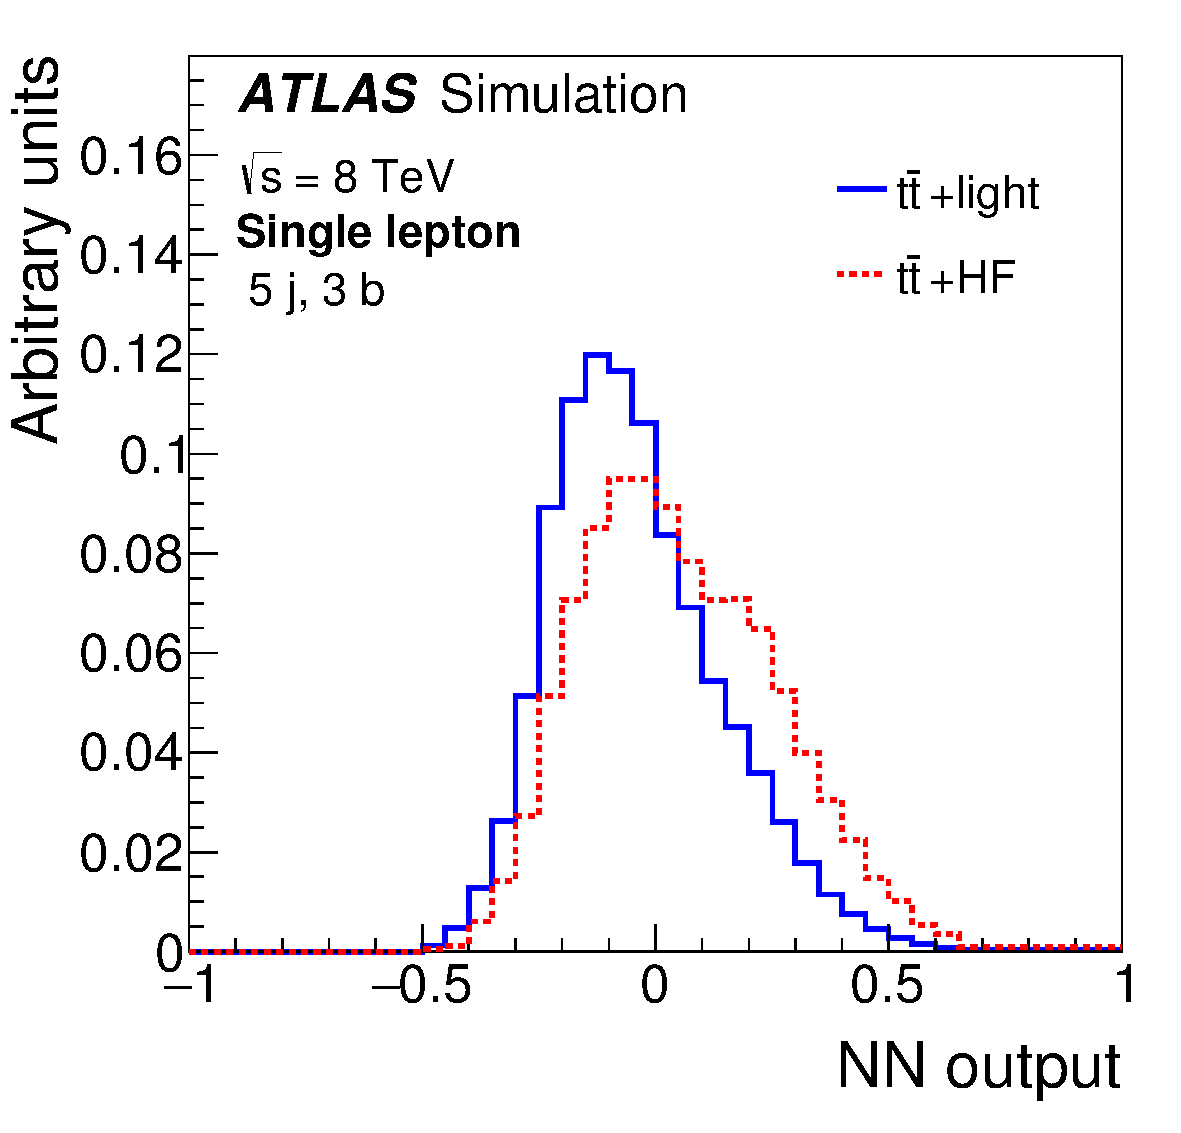
\includegraphics[width=\textwidth]{Analysis/Figures_ttH/NN125_5j_3b_kin_5_flav.pdf}\label{fig:Discriminationlj_a}
\caption{}\end{subfigure}
\begin{subfigure}{0.49\textwidth}
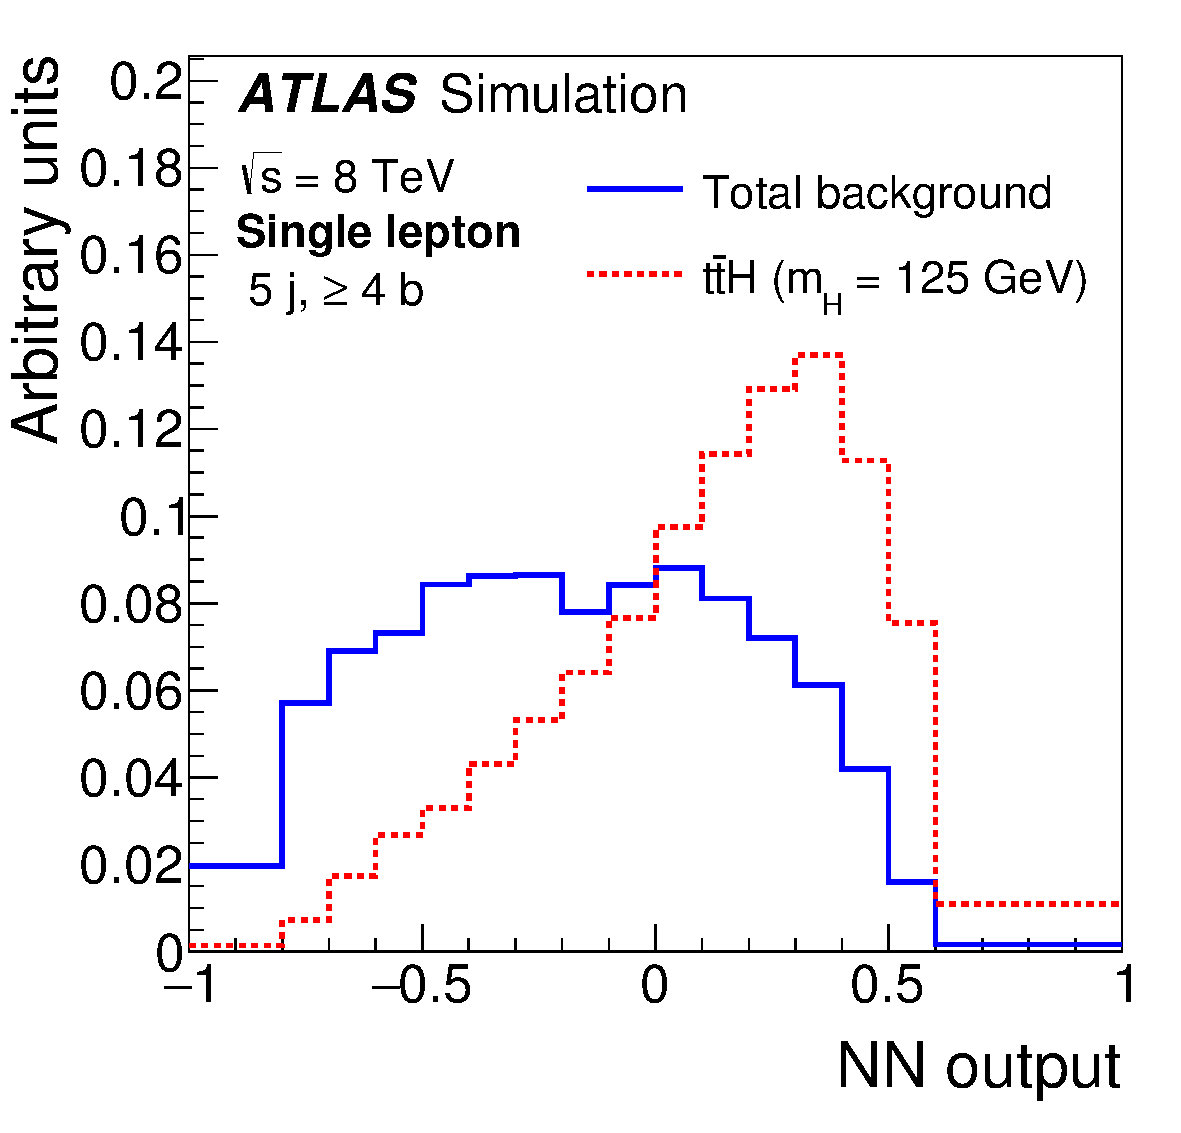
\includegraphics[width=\textwidth]{Analysis/Figures_ttH/NN125_5j_ge4b_kin_5_sep.pdf}\label{fig:Discriminationlj_b}\\
\caption{}\end{subfigure}
\begin{subfigure}{0.49\textwidth}
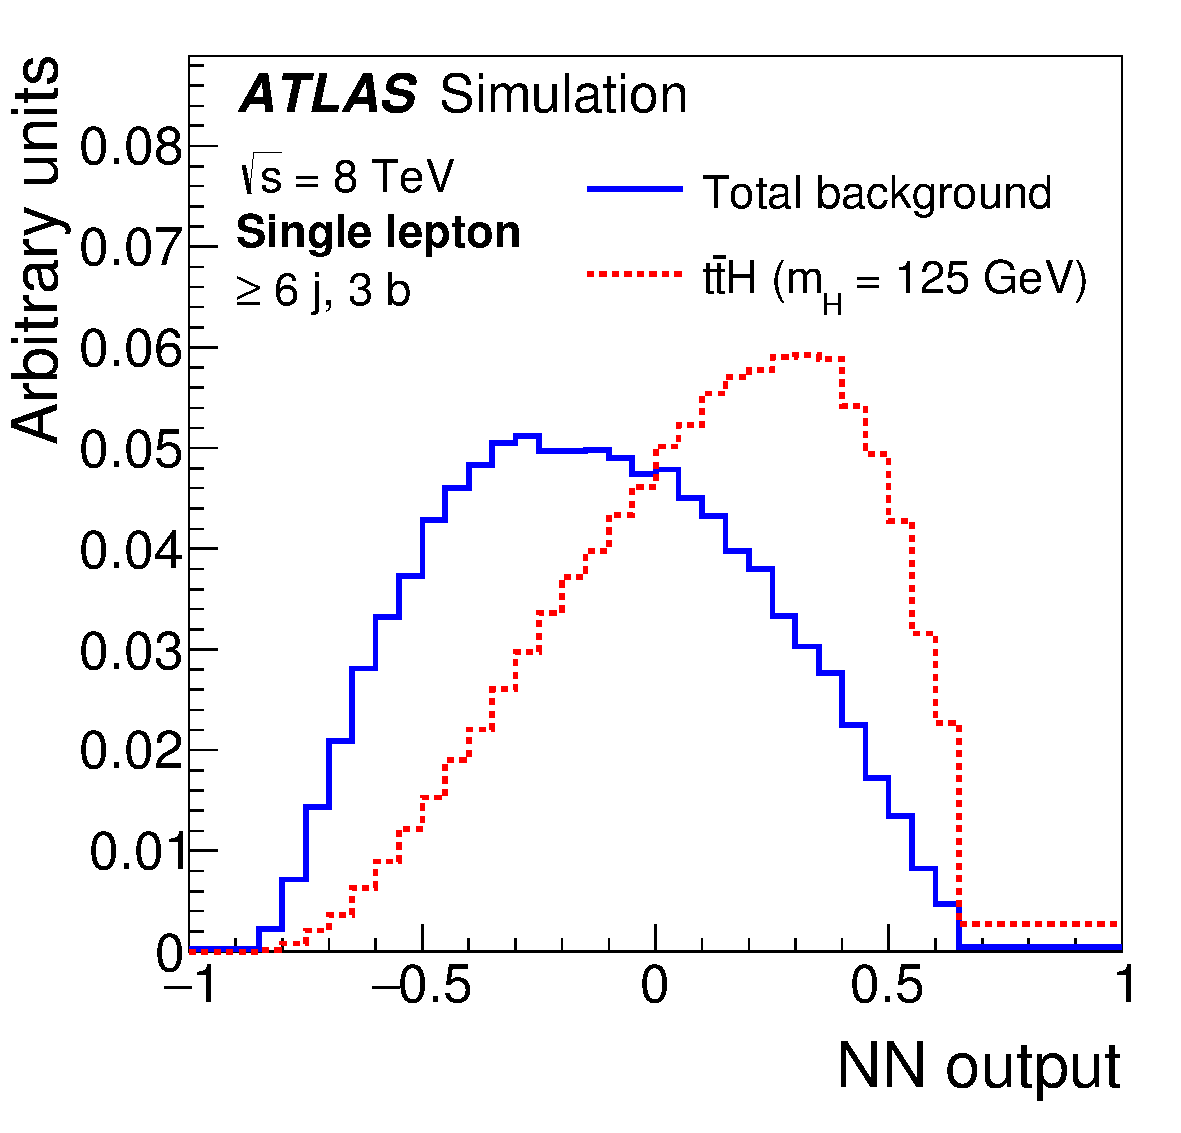
\includegraphics[width=\textwidth]{Analysis/Figures_ttH/NN125_6j_3b_kin_ME_6jincl_sep.pdf}\label{fig:Discriminationlj_c}
\caption{}\end{subfigure}
\begin{subfigure}{0.49\textwidth}
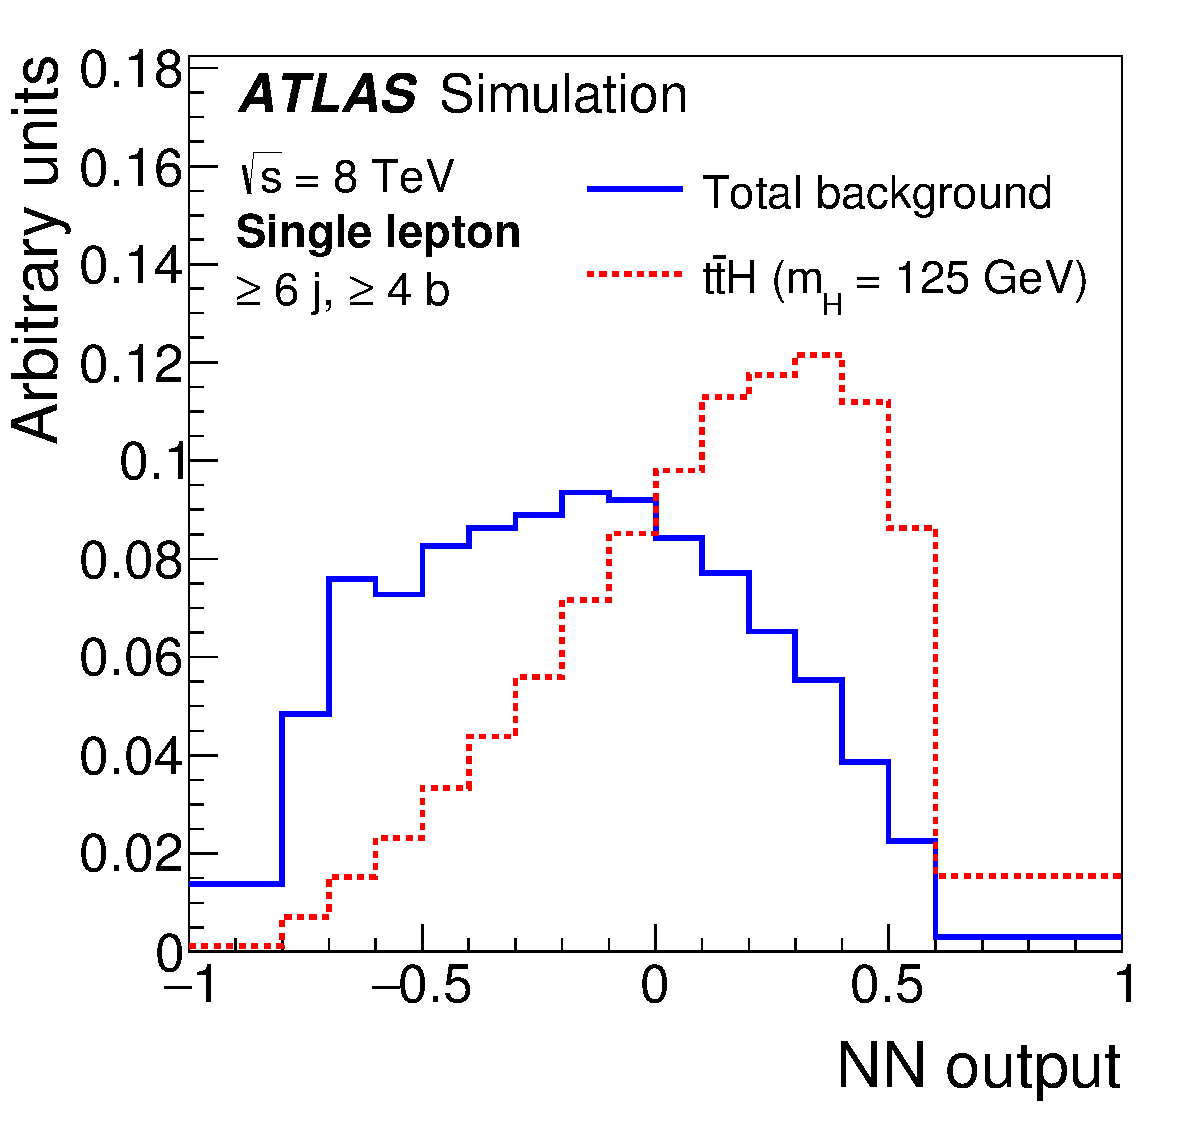
\includegraphics[width=\textwidth]{Analysis/Figures_ttH/NN125_6j_ge4b_kin_ME_6jincl_sep.pdf}\label{fig:Discriminationlj_d}
\caption{}\end{subfigure}
\caption{NN output for the different regions: (a) \fivethree, (b) \fivefour, (c) \sixthree\ and (d) \sixfour.
  In the \fivethree\ region the \ttbar+HF production is considered as signal and \ttbar+light as background
whereas in the rest of the regions the NN is trained to separate the \tth\ signal 
from the total background.  The distributions are normalized to unit area. }
\label{fig:Discriminationlj}
\end{figure}

 %%%%%%%%%%%%%%%%%%%%%%%% - INPUT
\subsection{Matrix element method}
\label{subsec:MEM}
The matrix element method~\cite{kondo1} links directly
theoretical calculations and observed quantities,  making the most complete 
use of the kinematic information in an event. 
%has been used by the D0 and CDF 
%collaborations for precision measurements of the top quark 
%mass~\cite{d0_topmass,cdf_topmass} and for the observations of single top 
%quark production~\cite{d0_stop,cdf_stop}. Recently this technique has 
%been used for the \tth\ search by the
%CMS experiment~\cite{CMSMEM}. 

Given an observation, defined by the four-momentum vectors of all final-state objects at reconstruction level, $\MB{x}$,
the method calculates the probability 
of the event to be consistent with physics process $i$ 
described by a set of parameters $\MB{\alpha}$. 
This probability density function $P_i \left ( \MB{x} | \MB{\alpha} \right )$
is defined as:

\begin{equation}
P_i\left(\MB{x}|\MB{\alpha}\right) = \frac{(2\pi)^4}{\sigma_i^{\mathrm{exp}}\left(\MB{\alpha}\right)} 
\int \dif{\SUB{p}{a}} \dif{\SUB{p}{b}} \; f(\SUB{p}{a}) f(\SUB{p}{b}) \;
 \frac{\left|\mathcal{M}_{i}\left(\MB{y}|\MB{\alpha}\right)\right|^2}{\mathcal{F}} \;
W\left(\MB{y}|\MB{x}\right) \; \dif{\Phi_N}\left(\MB{y}\right)~,
\end{equation}

\noindent and is obtained by numerical integration
over the entire phase space of the initial- and final-state particles. 
The transfer functions $W\left(\MB{y}|\MB{x}\right)$ map the detector quantities
$\MB{x}$ to the parton level quantities $\MB{y}$.
The transition matrix 
element $\mathcal{M}_{i}\left(\MB{y}|\MB{\alpha}\right)$ is defined by the Feynman diagrams of the hard process considered, $i$. 
The flux factor $\mathcal{F}$ and the Lorentz-invariant phase space element 
$\dif{\Phi_N}$ describe the kinematics of the process, and $f\left(\SUB{p}{a,b}\right)$ are parton distribution functions.  
Finally, the \xsec\ 
$\sigma_i^{\mathrm{exp}}$ normalizes $P_i$ to unity 
taking acceptance and efficiency into account.

The assignment of reconstructed objects to final-state partons in the hard process 
contains multiple ambiguities. The process probability is computed for each allowed assignment permutation 
of the jets to the final-state quarks of the hard process.
A process likelihood function can then be built 
by summing the process probabilities for the $N_{p}$ allowed assignment 
permutations:

\begin{equation}
\mathcal{L}_{i}  \left (\MB{x}|\MB{\alpha}\right )  = \sum_{p=1}^{N_{p}} \strut P_{i}^{p}
\left (\MB{x}|\MB{\alpha} \right ). 
\label{eq:SSLL}
\end{equation}

The process probability densities are used to distinguish signal from 
background events by calculating the likelihood ratio of the signal and 
background processes contributing with fractions $f_{\textrm{bkg}}$,

\begin{equation}
r_{\textrm{sig}} \left  ( \MB{x} | \MB{\alpha} \right ) = 
\frac{\mathcal{L}_{\textrm{sig}} \left (\MB{x}|\MB{\alpha} \right )}
{\sum\limits_{\textrm{bkg}} f_{\textrm{bkg}} \mathcal{L}_{\textrm{bkg}} 
\left (\MB{x}|\MB{\alpha} \right ) } \label{eq:neyman}~. 
\end{equation} 

This ratio, according to the Neyman--Pearson lemma~\cite{neymanpearson}, is the 
most powerful discriminant between signal and background processes. In the analysis, 
this variable is used as input to the NN along with other kinematic variables. 
 
The integration is performed with \textsc{VEGAS}~\cite{VEGAS} using adaptive MC techniques~\cite{gsl}.
Matrix element calculations are generated with \madgraphfive\ at LO. 
The transfer functions are obtained from simulation~\cite{klfitter} and the parton
distribution functions are taken from the {\sc CTEQ6L1} set from the \textsc{LHAPDF} package~\cite{lhapdf}.

%The integration is performed using \textsc{VEGAS}~\cite{VEGAS}.  Due to the complexity and 
%high dimensionality, adaptive MC techniques~\cite{gsl}, 
%simplifications and approximations are needed to obtain results 
%within a reasonable computing time.
%In particular, only the numerically most significant contributing helicity states of a 
%process hypothesis for a given event,  
%identified at the start of each integration, are evaluated. This does not 
%perceptibly decrease the separation power but reduces the calculation time by 
%more than an order of magnitude. 
%Furthermore, several approximations are made to improve the {\sc VEGAS} convergence rate. 
%Firstly, the dimensionality of integration is reduced by assuming that the final-state object 
%directions in \eta{} and $\phi$ as well as charged lepton momenta are well measured, and therefore 
%the corresponding transfer functions are represented by $\delta$ functions. 
%The total momentum conservation and a negligible transverse momentum of the 
%initial-state partons allow for further reduction.
%Secondly, kinematic transformations are utilised to optimise the integration over the remaining 
%phase space by aligning the peaks of the integrand with the integration dimensions. 
%The narrow-width approximation is applied to the leptonically decaying $W$ boson. 
%This leaves three $b$-quark energies, one light-quark energy, the hadronically decaying 
%$W$ boson mass and the invariant mass of the two $b$-quarks
%originating from either the Higgs boson for the signal  
%or a gluon for the background as the remaining parameters which define the integration phase space.
%The total integration volume is restricted based  upon the observed values and the width 
%of the transfer functions and of the 
%propagator peaks in the matrix elements. Finally, the likelihood 
%contributions of all allowed assignment permutations are coarsely integrated, and  
%only for the leading twelve assignment permutations is the full integration performed, 
%with a required precision decreasing according to their relative contributions.

\begin{figure}[tb!]
\begin{center}
  \begin{subfigure}{0.49\textwidth}
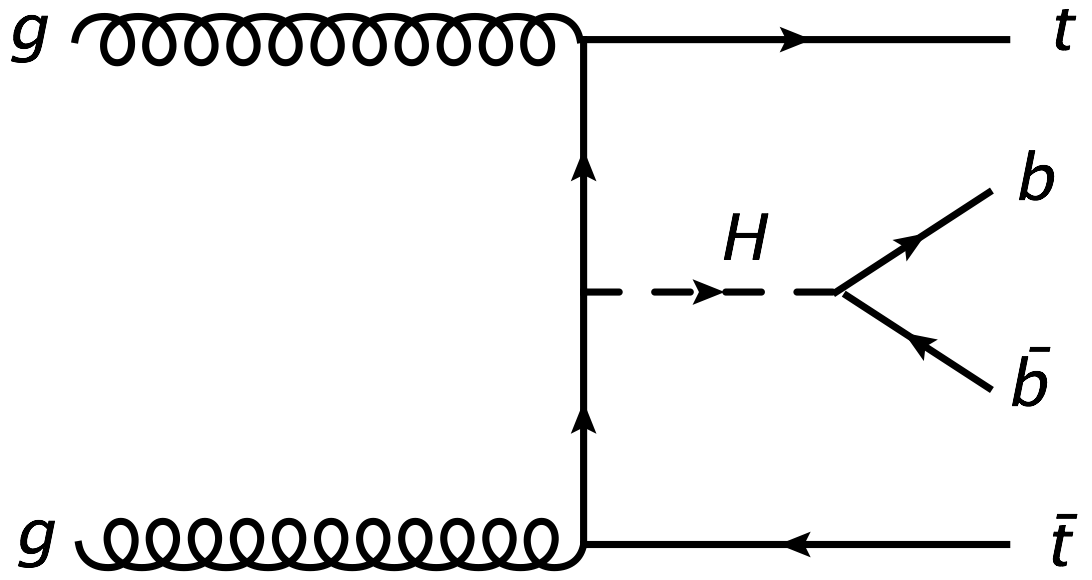
\includegraphics[width=\textwidth]{Analysis/Figures_ttH/ttHbb_fusion.png}
\caption{}\label{fig:feyn_ttH_1} \end{subfigure}
%\begin{subfigure}{0.49\textwidth} %Change caption
%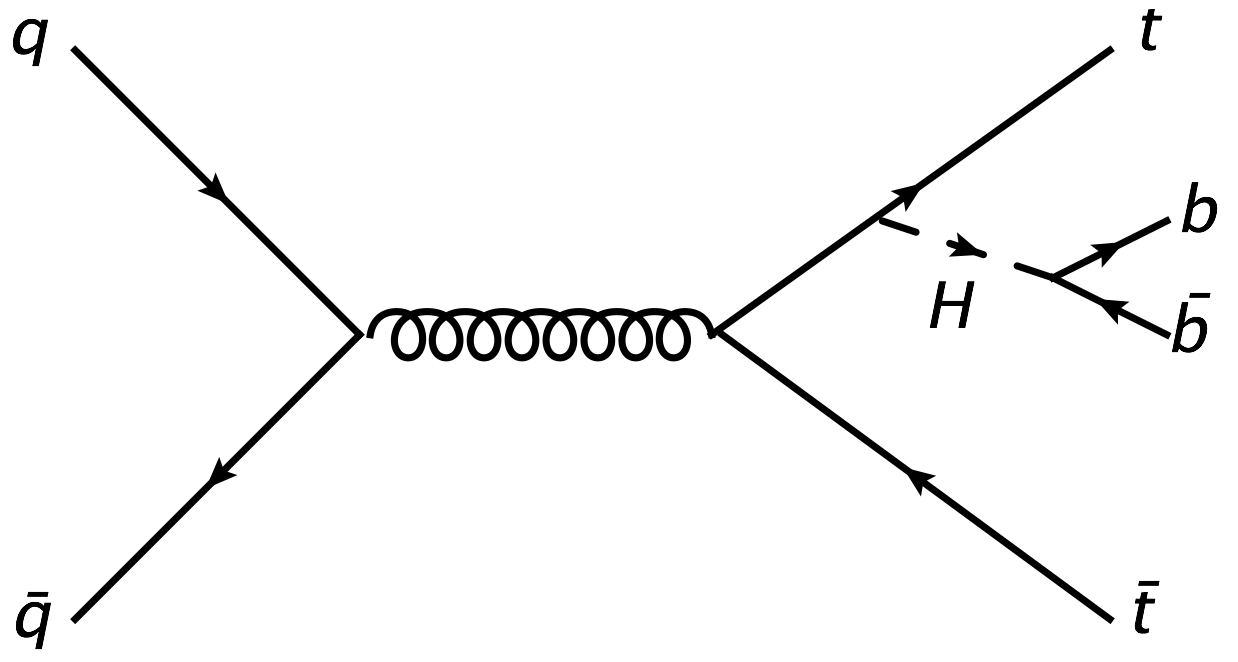
\includegraphics[width=\textwidth]{Analysis/Figures_ttH/ttHbb_radiation.png} 
%\caption{}\label{fig:feyn_ttH_2} \end{subfigure}
\begin{subfigure}{0.49\textwidth}
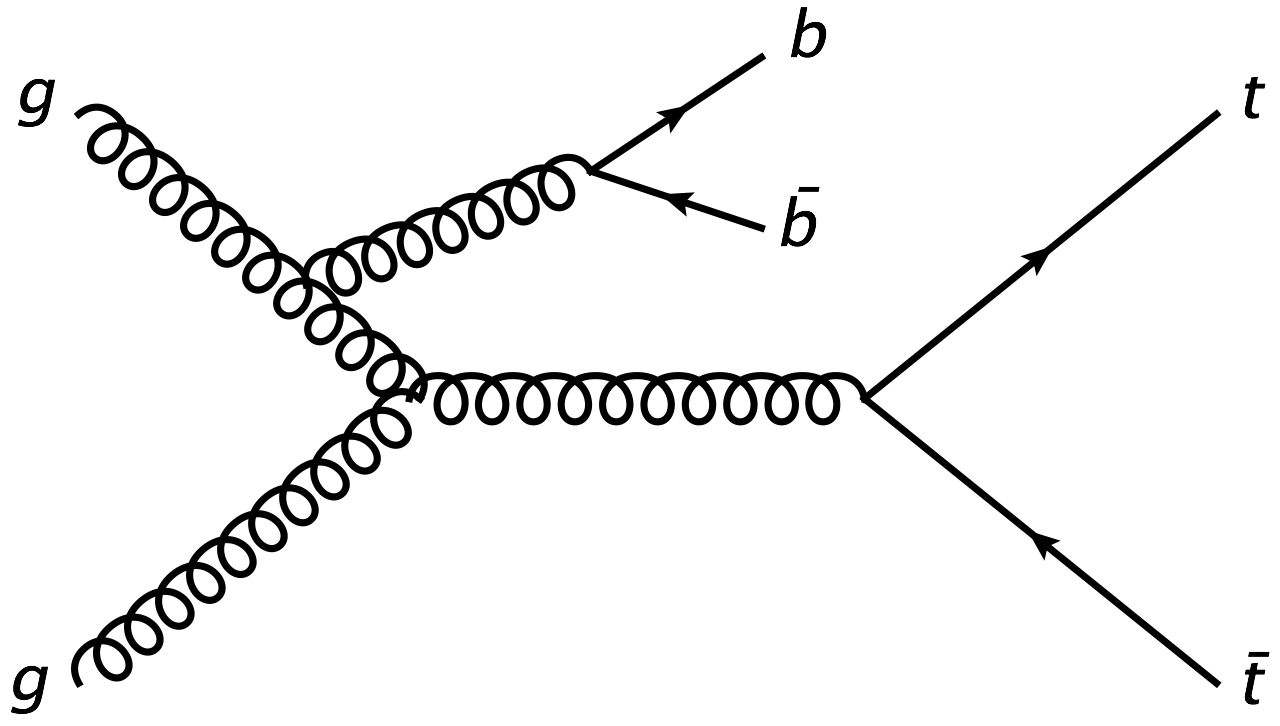
\includegraphics[width=\textwidth]{Analysis/Figures_ttH/ttbb.png}
\caption{}\label{fig:feyn_ttbb} \end{subfigure}
\caption{(a) Representative tree-level Feynman diagrams for the production of the Higgs boson in association with a top pair (\tth) and the subsequent decay of the Higgs to \bbbar, (b) and for the main background \ttbar+\bbbar. 
}
\label{fig:feynman}
\end{center}
\end{figure}

The signal hypothesis is defined as a SM Higgs boson produced in association
with a top-quark pair as shown in figure~\ref{fig:feyn_ttH_1}. 
The Higgs boson is required to decay into \bbbar, while the top-quark pair decays 
into the single-lepton channel. 
For the background hypothesis, only the diagrams of the irreducible 
\ttbb\ background are considered, as shown in figure~\ref{fig:feyn_ttbb}. Since it dominates the most signal-rich analysis regions, 
the inclusion of other processes does not improve the separation 
between signal and background. 
%No gluon radiation from the 
%final-state quarks is  
%allowed, since these are kinematically suppressed and difficult to treat in any kinematic 
%transformation aiming for phase-space alignment during the integration process.
%In the definition of the signal and background hypothesis the LO diagrams are 
%required to have a top-quark pair as an intermediate state resulting in exactly 
%four $b$-quarks, two light quarks, one charged lepton (electron or muon) and one neutrino 
%in the final state. Assuming lepton universality and invariance under charge 
%conjugation,  
%diagrams of only one lepton flavour and of only negative charge (electron) are considered.
The probability density function calculation of the signal and background is only performed in the \sixthree\ 
and \sixfour\ regions. 

Only six reconstructed 
jets are considered in the calculation: 
the four jets with the highest value of the probability to be a $b$-jet returned by the 
$b$-tagging algorithm (i.e. the highest $b$-tagging weight) 
and two of the remaining jets with an 
invariant mass closest to the $W$ boson mass of 80.4 \gev. 
%If a jet is $b$-tagged it cannot be 
%assigned to a light quark in the matrix element description. In the case of more than four 
%$b$-tagged jets, only the four with the highest $b$-tagging weight are treated as $b$-tagged. 
Assignment permutations between the two light quarks of the hadronically decaying $W$ 
boson and between 
the two $b$-quarks originating from the Higgs boson or gluon result in the same 
likelihood value and are thus not considered.
As a result there are in total 12 and 36 assignment permutations in the \sixfour\ 
and \sixthree\ regions, respectively, which need to be integrated.

Using the \tth\ process as the signal hypothesis and the \ttbb\ process as the 
background hypothesis, a slightly modified version of equation~(\ref{eq:neyman}) is used to define 
the likelihood ratio $D1$:

\begin{equation}
 D1=\frac{\mathcal{L}_{t\bar{t}H}}{{\mathcal{L}_{t\bar{t}H}} + 
 \alpha \cdot \mathcal{L}_{t\bar{t}+b\bar{b}}}\
\label{eq:ME_D1} ,
\end{equation}

\noindent where $\alpha=0.23$ is a relative normalization factor chosen to optimize the
performance of the discriminant given the finite bin sizes of the $D1$ distribution. 
In this definition, 
signal-like and background-like events have $D1$ values close to one and zero, 
respectively.   
The logarithm of the summed signal likelihoods defined by equation~(\ref{eq:SSLL}) 
and the ratio $D1$ are included in the 
NN training in both the \sixthree\ and \sixfour\ regions. 

The $D1$ variable provides the best separation between the
\tth\ signal and the dominant \ttbb\ background in the \sixfour\ region, and the 
SSLL variable introduces further separation to the rest of the backgrounds.  
Figure~\ref{fig:MEM_separation} shows the discrimination power of the $D1$ and SSLL variables in the \sixthree\ and \sixfour\ regions.
\begin{figure}[tb!]
  \centering
  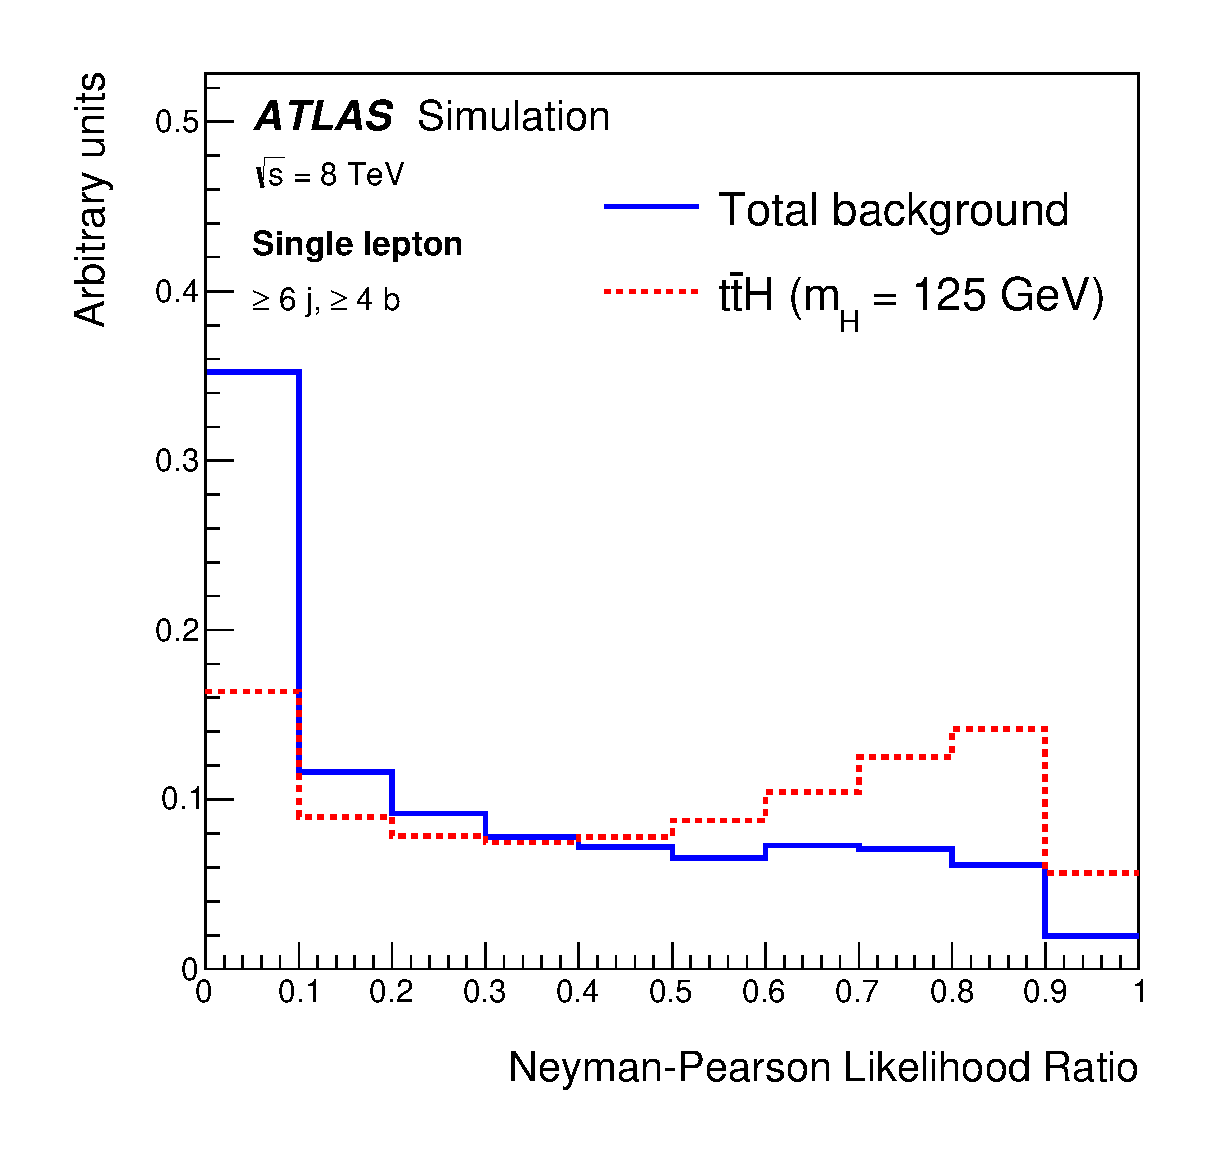
\includegraphics[width=0.49\textwidth]{Analysis/Figures_ttH/ME_D1_6jincl_sep.eps}
  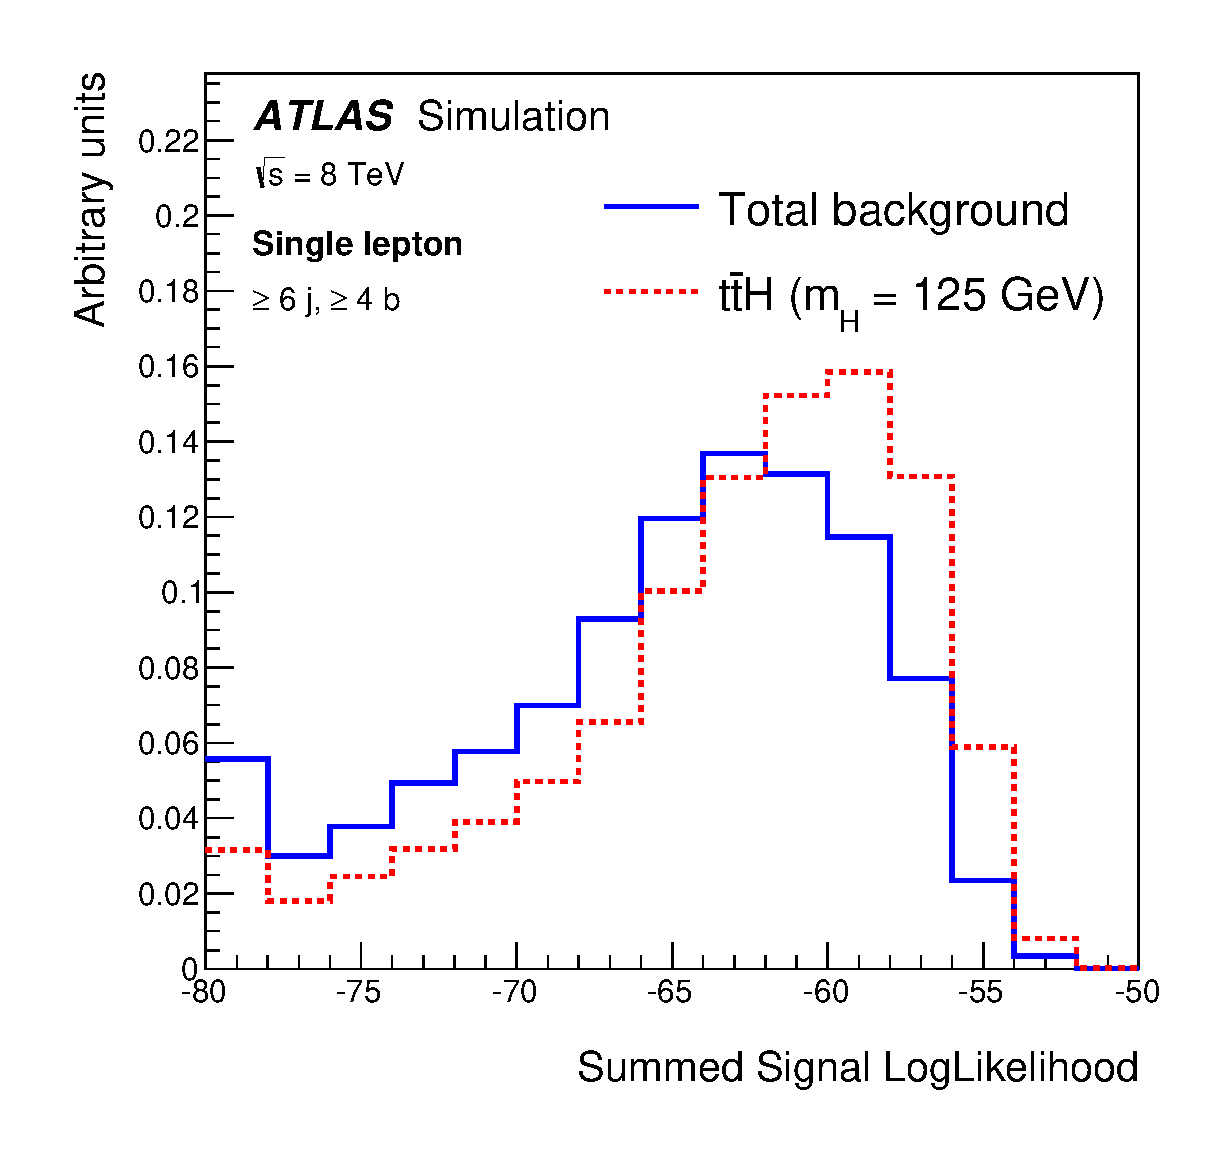
\includegraphics[width=0.49\textwidth]{Analysis/Figures_ttH/ME_SLL_6jincl_sep.eps}
  \caption{Expected distributions for $D1$ and SSLL in the \tth\ signal and total background in the \sixfour\ region.}
  \label{fig:MEM_separation}
\end{figure}

 %%%%%%%%%%%%%%%%%%%%%%%% - INPUT

\subsection{Fit results}
\label{subsec:fit_ttH}
A fit to the data in the nine analysis regions is performed under the signal-plus-background hypothesis, and the fitted NP are shown in figure~\ref{fig:ttH_fit}.
For each NP, the fitted value represents the preferred shift with respect to the nominal prediction in units of its prior uncertainty, 
whereas the fitted error represents the post-fit uncertainty in units of the prior uncertainty. 
The corresponding correlation matrix for the
fitted NP can be found in figure~\ref{fig:corrmat_ttH}.
The fitted value for the signal strength is: $\mu= 1.2 \pm 1.3$, and the expected uncertainty for the signal strength (assuming $\mu = 1$) is $\pm 1.2$.

\begin{figure}[!tp]
\begin{center}
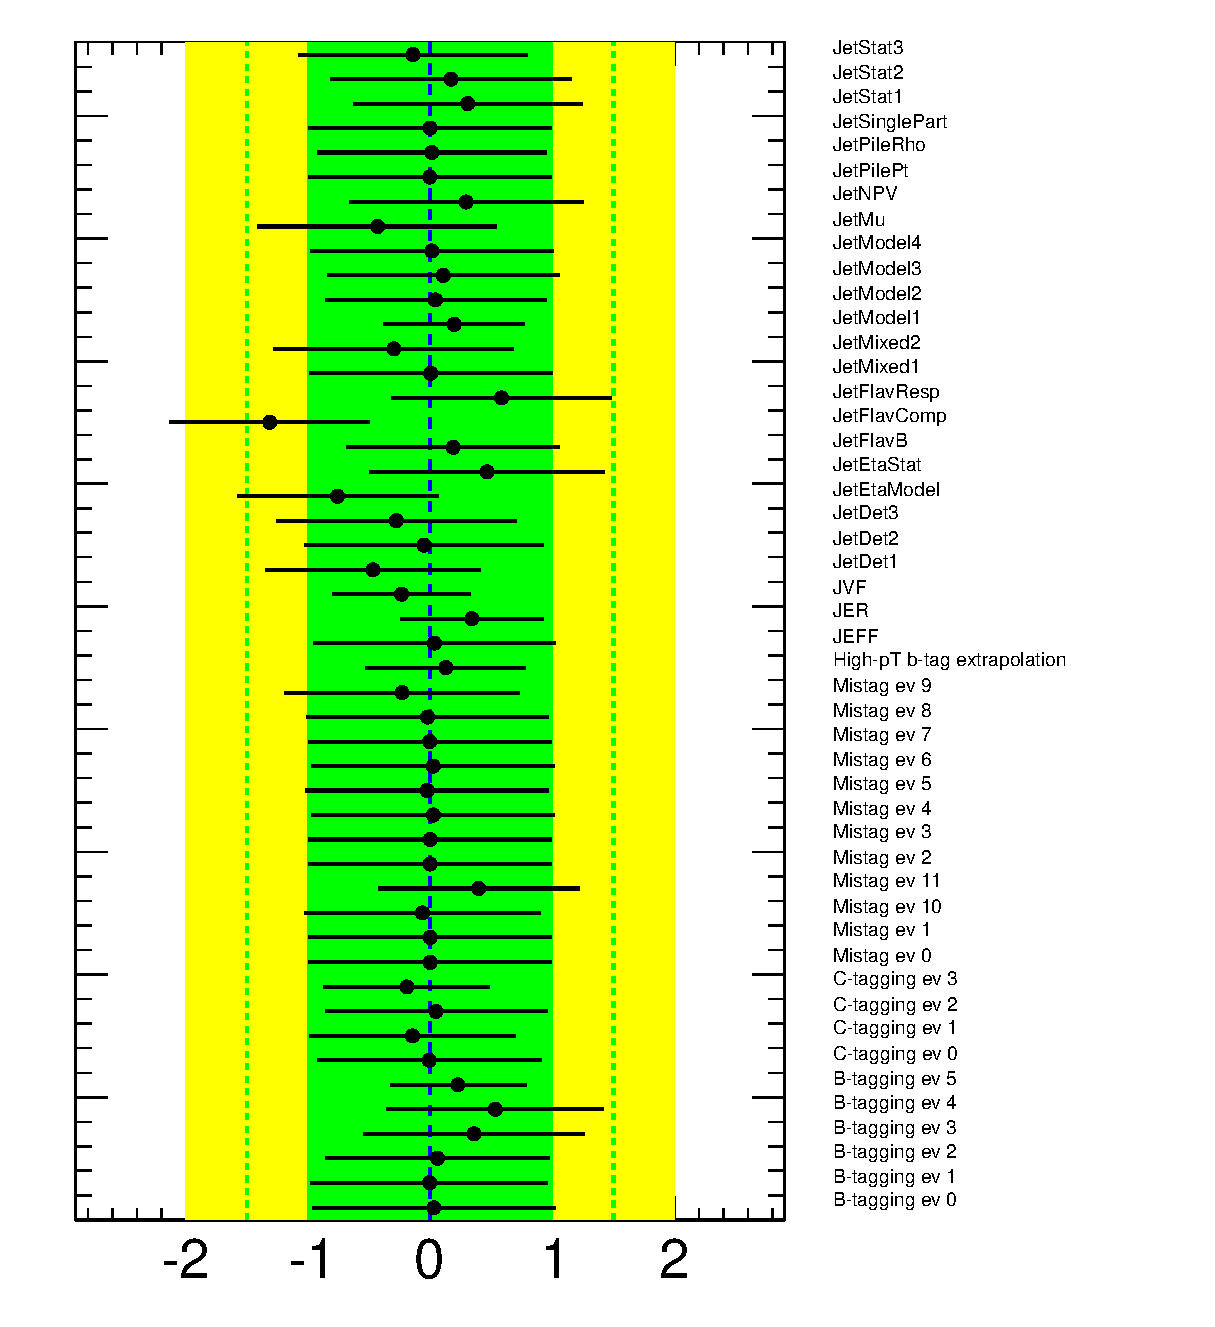
\includegraphics[trim=0cm 0cm 1.5cm 0cm, clip=true, width=0.49\textwidth]{Analysis/Figures_ttH/detectorUNCljets_tesis.eps}
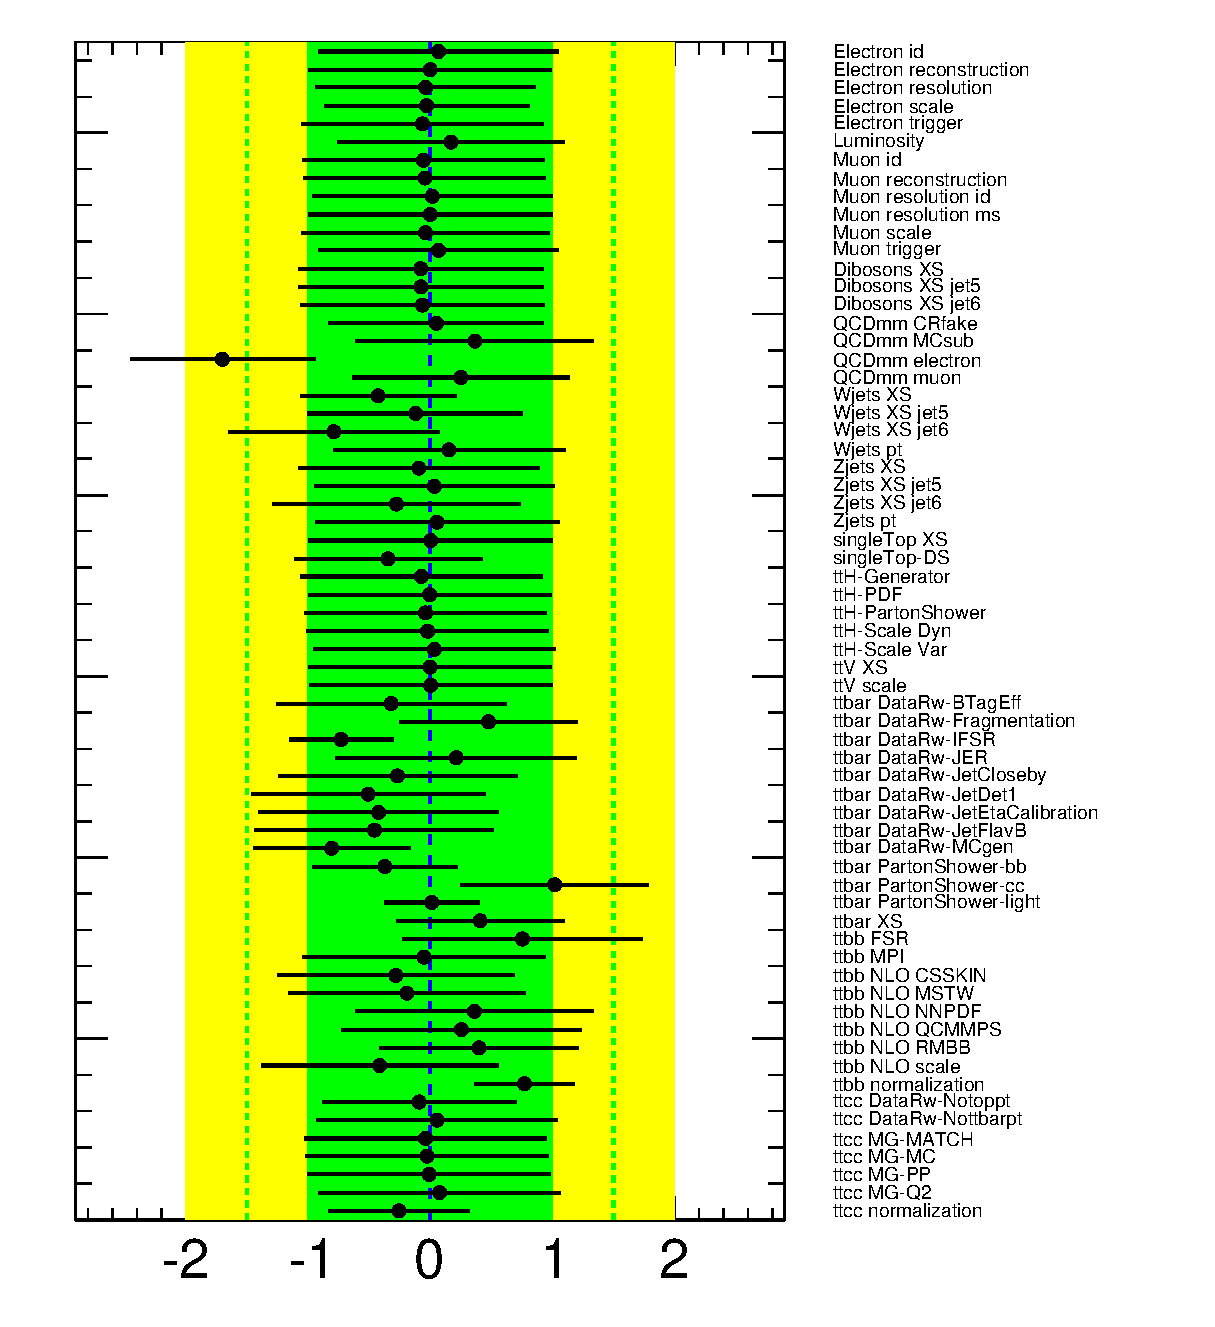
\includegraphics[trim=0cm 0cm 1.5cm 0cm, clip=true, width=0.49\textwidth]{Analysis/Figures_ttH/otherUNCljets_tesis.eps}
\caption{Fitted NPs under the signal-plus-background hypothesis. A detailed description of the naming of the NPs can be found in appendix~\ref{app:glossary}.}
\label{fig:ttH_fit} 
\end{center}
\begin{center}
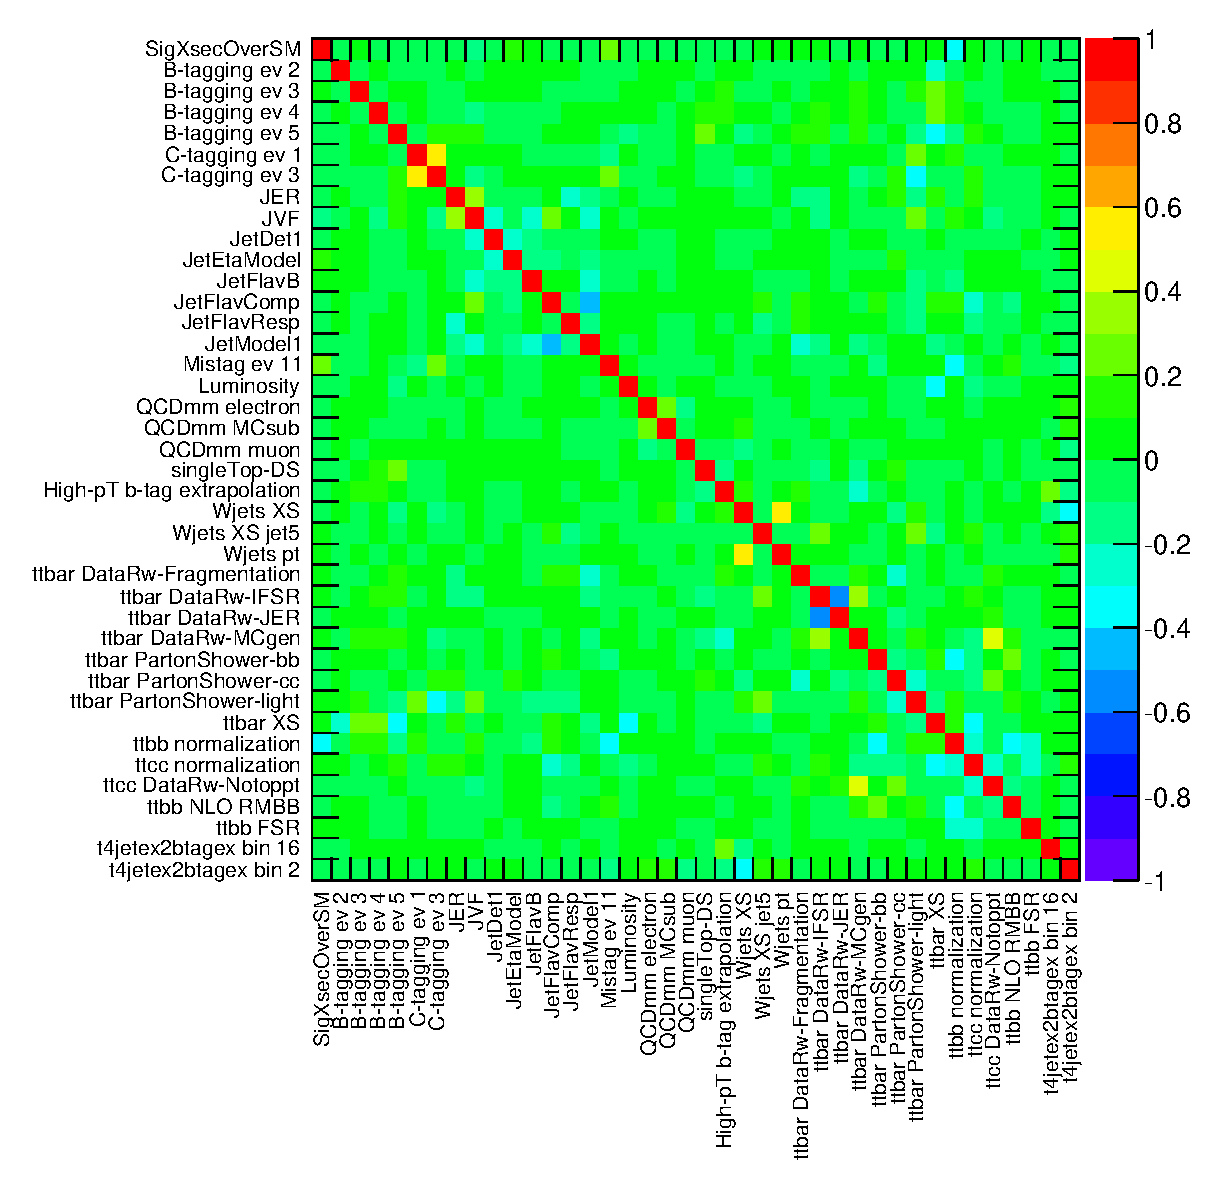
\includegraphics[width=0.6\textwidth]{Analysis/Figures_ttH/CorrMat_ttH.eps}
\caption{Correlation matrix corresponding to the fit under the signal-plus-background hypothesis.
Only NPs with a correlation coefficient of at least 20\% with any other parameter are displayed.}
\label{fig:corrmat_ttH} 
\end{center}
\end{figure}

Figures~\ref{fig:postfit_ttH_1} and~\ref{fig:postfit_ttH_2} show the comparison of data and prediction for the $\hthad$ and NN distributions
in each of the regions considered, after the fit to data.
Compared to the pre-fit distributions, the total background uncertainty is significantly
reduced after the fit, not only in the background-dominated channels, but also in the signal-rich
channels, resulting in an increase in the search sensitivity. The reduced uncertainty results from the significant constraints on some
systematic uncertainties, as well as the anti-correlations among sources of systematic uncertainty 
resulting from the fit to the data.
The corresponding post-fit yields per channel can be found in table~\ref{tab:Postfit_EventsTable_lj}.

\begin{figure}[tpb!]
  \centering
  \begin{subfigure}{0.44\textwidth}
  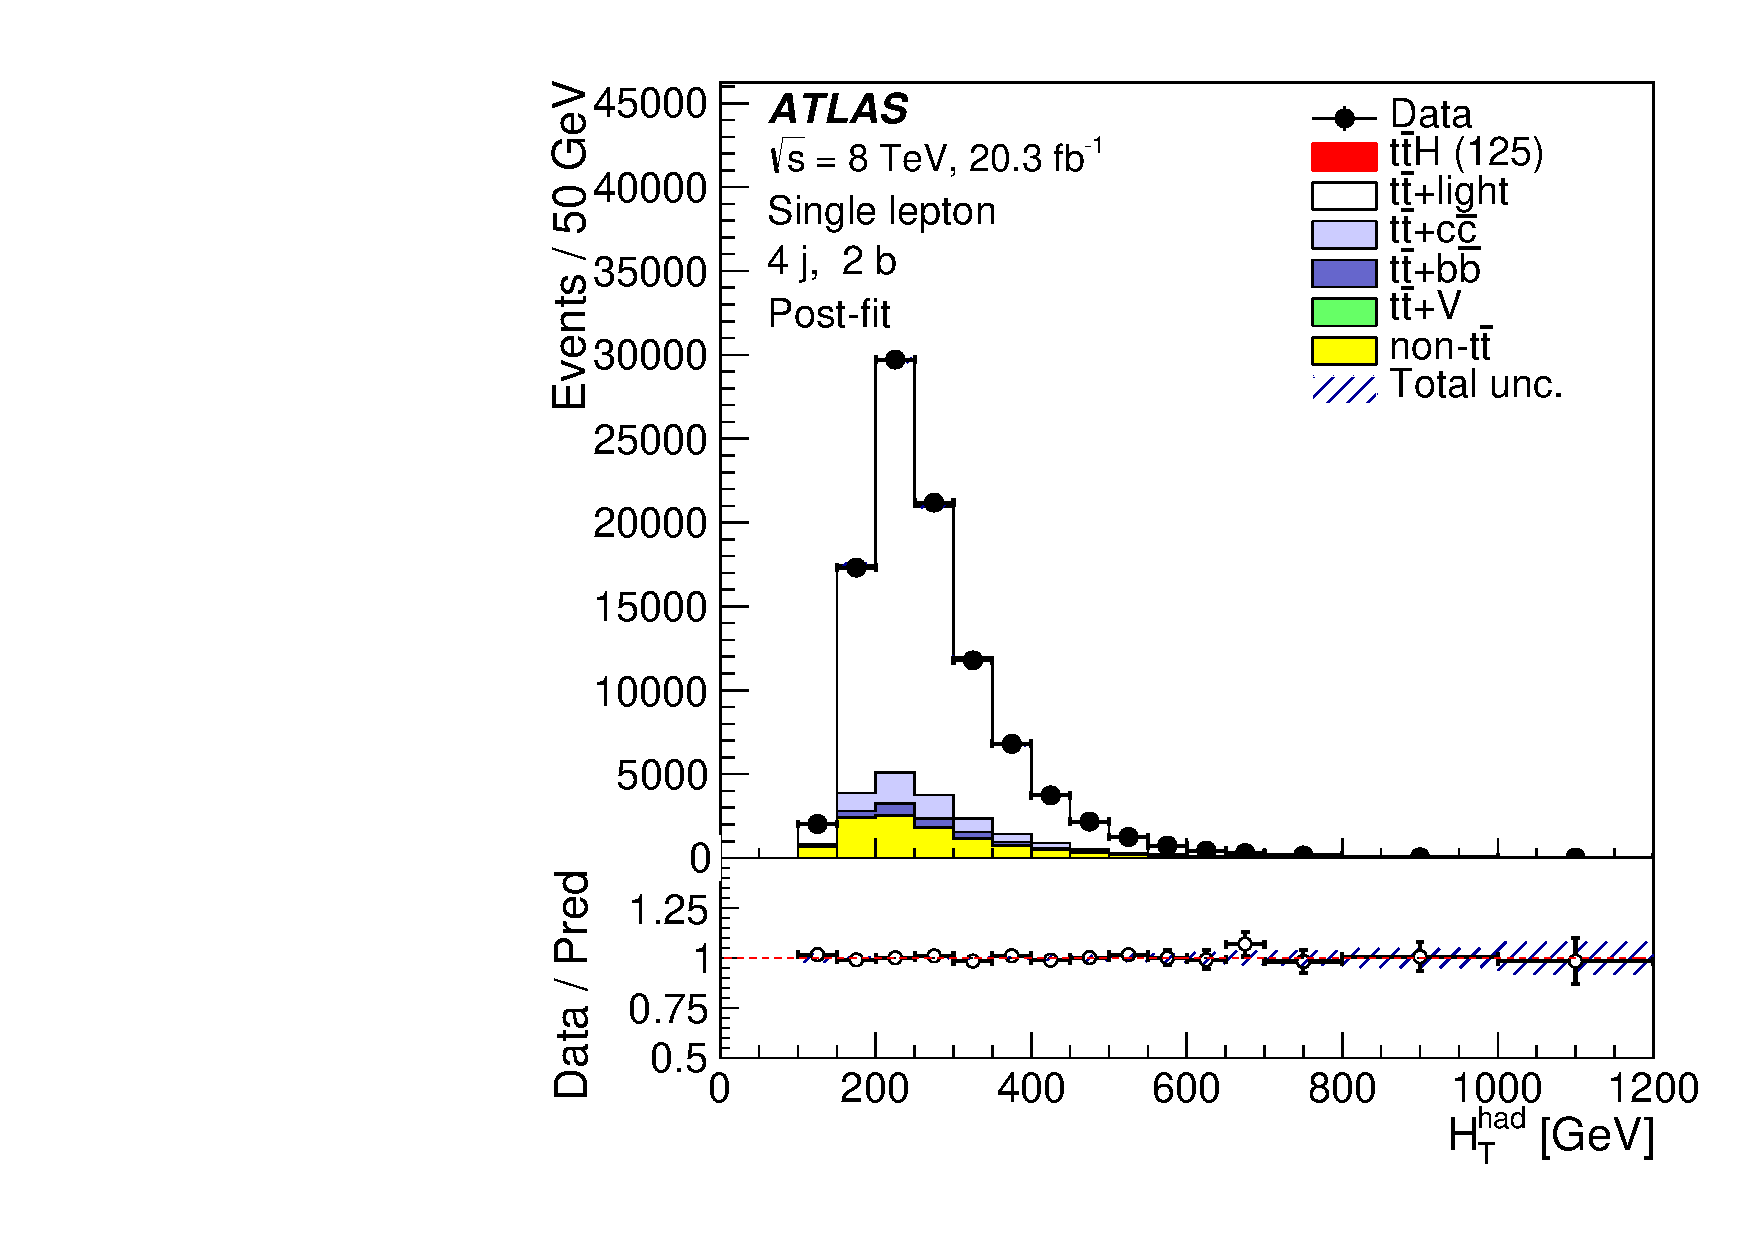
\includegraphics[width=\textwidth]{Analysis/Figures_ttH/HTHad_4jetex2btagex8TeV.pdf}
  \caption{}\end{subfigure}
  \begin{subfigure}{0.44\textwidth}
  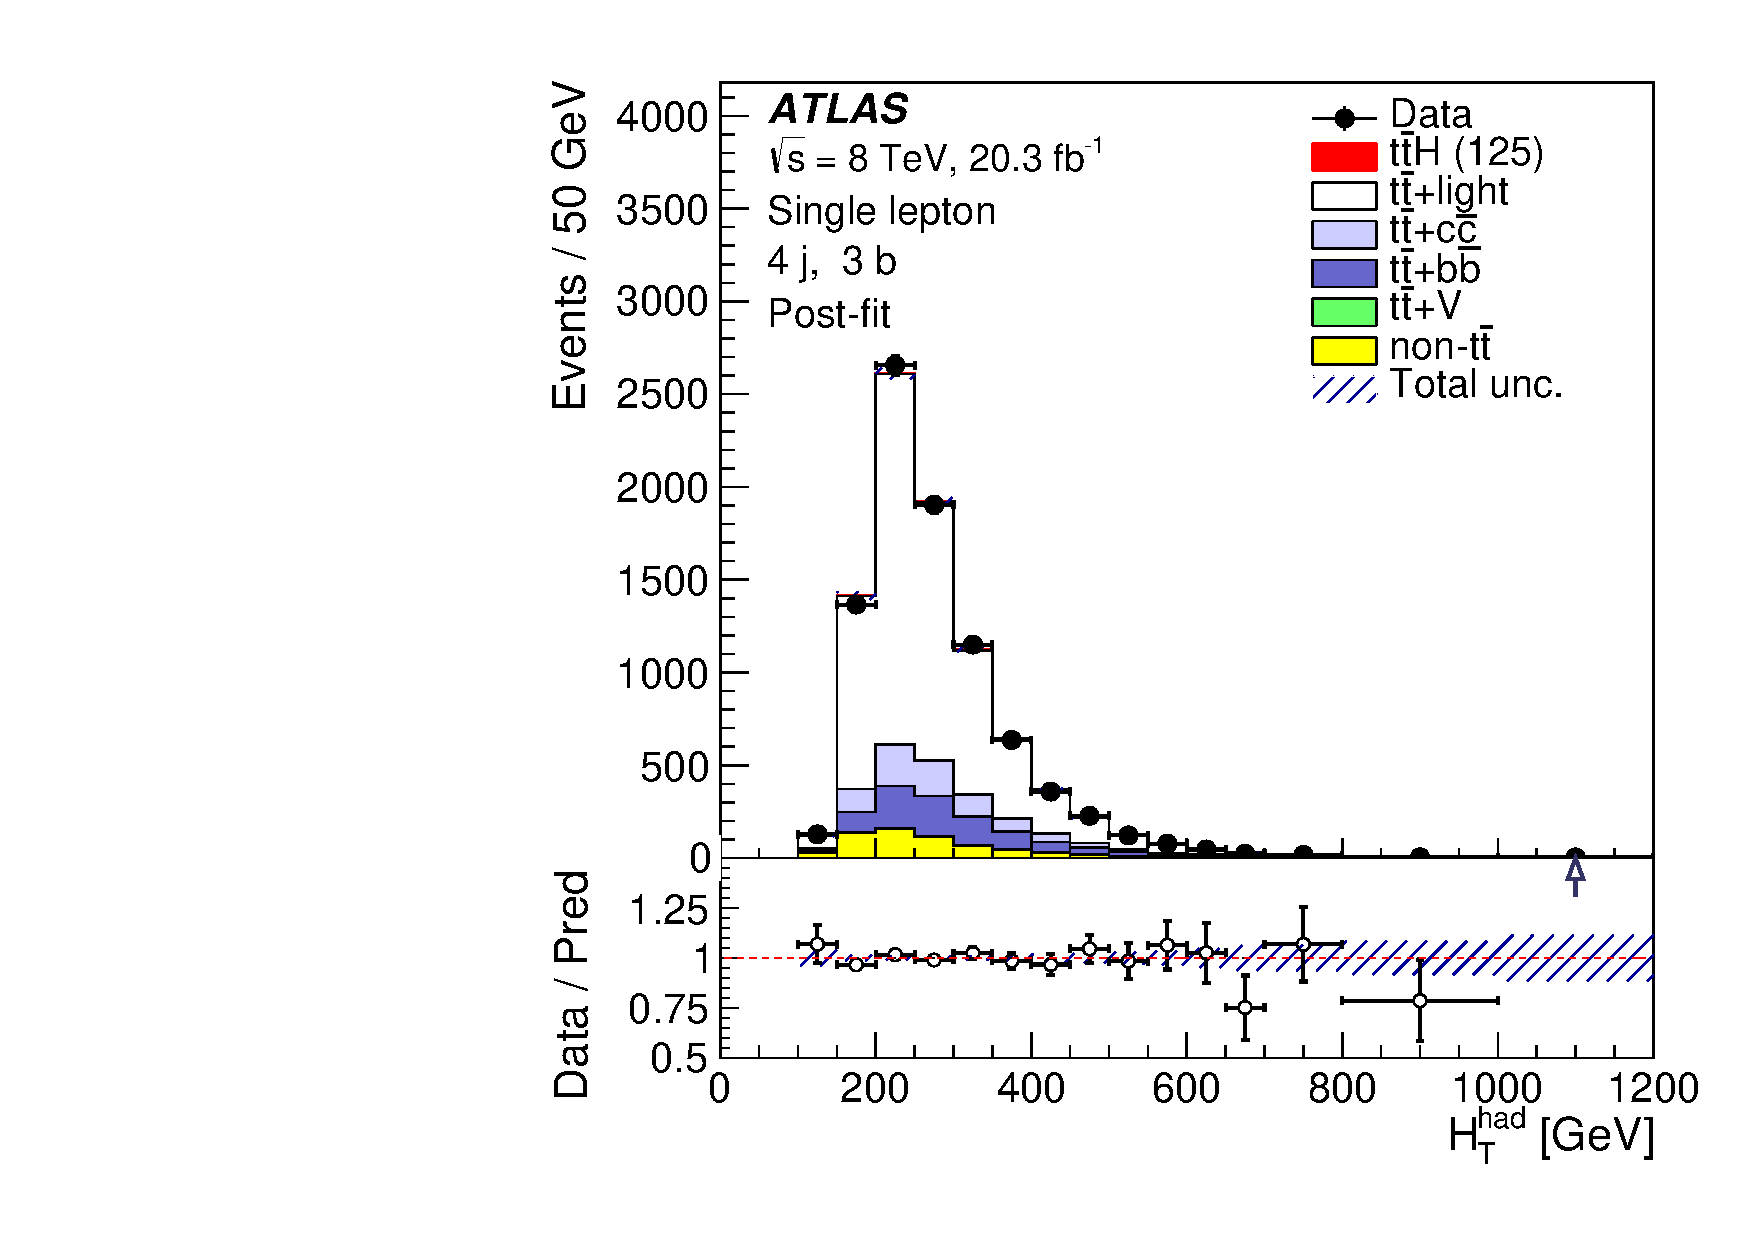
\includegraphics[width=\textwidth]{Analysis/Figures_ttH/HTHad_4jetex3btagex8TeV.pdf}
  \caption{}\end{subfigure}
  \begin{subfigure}{0.44\textwidth}
  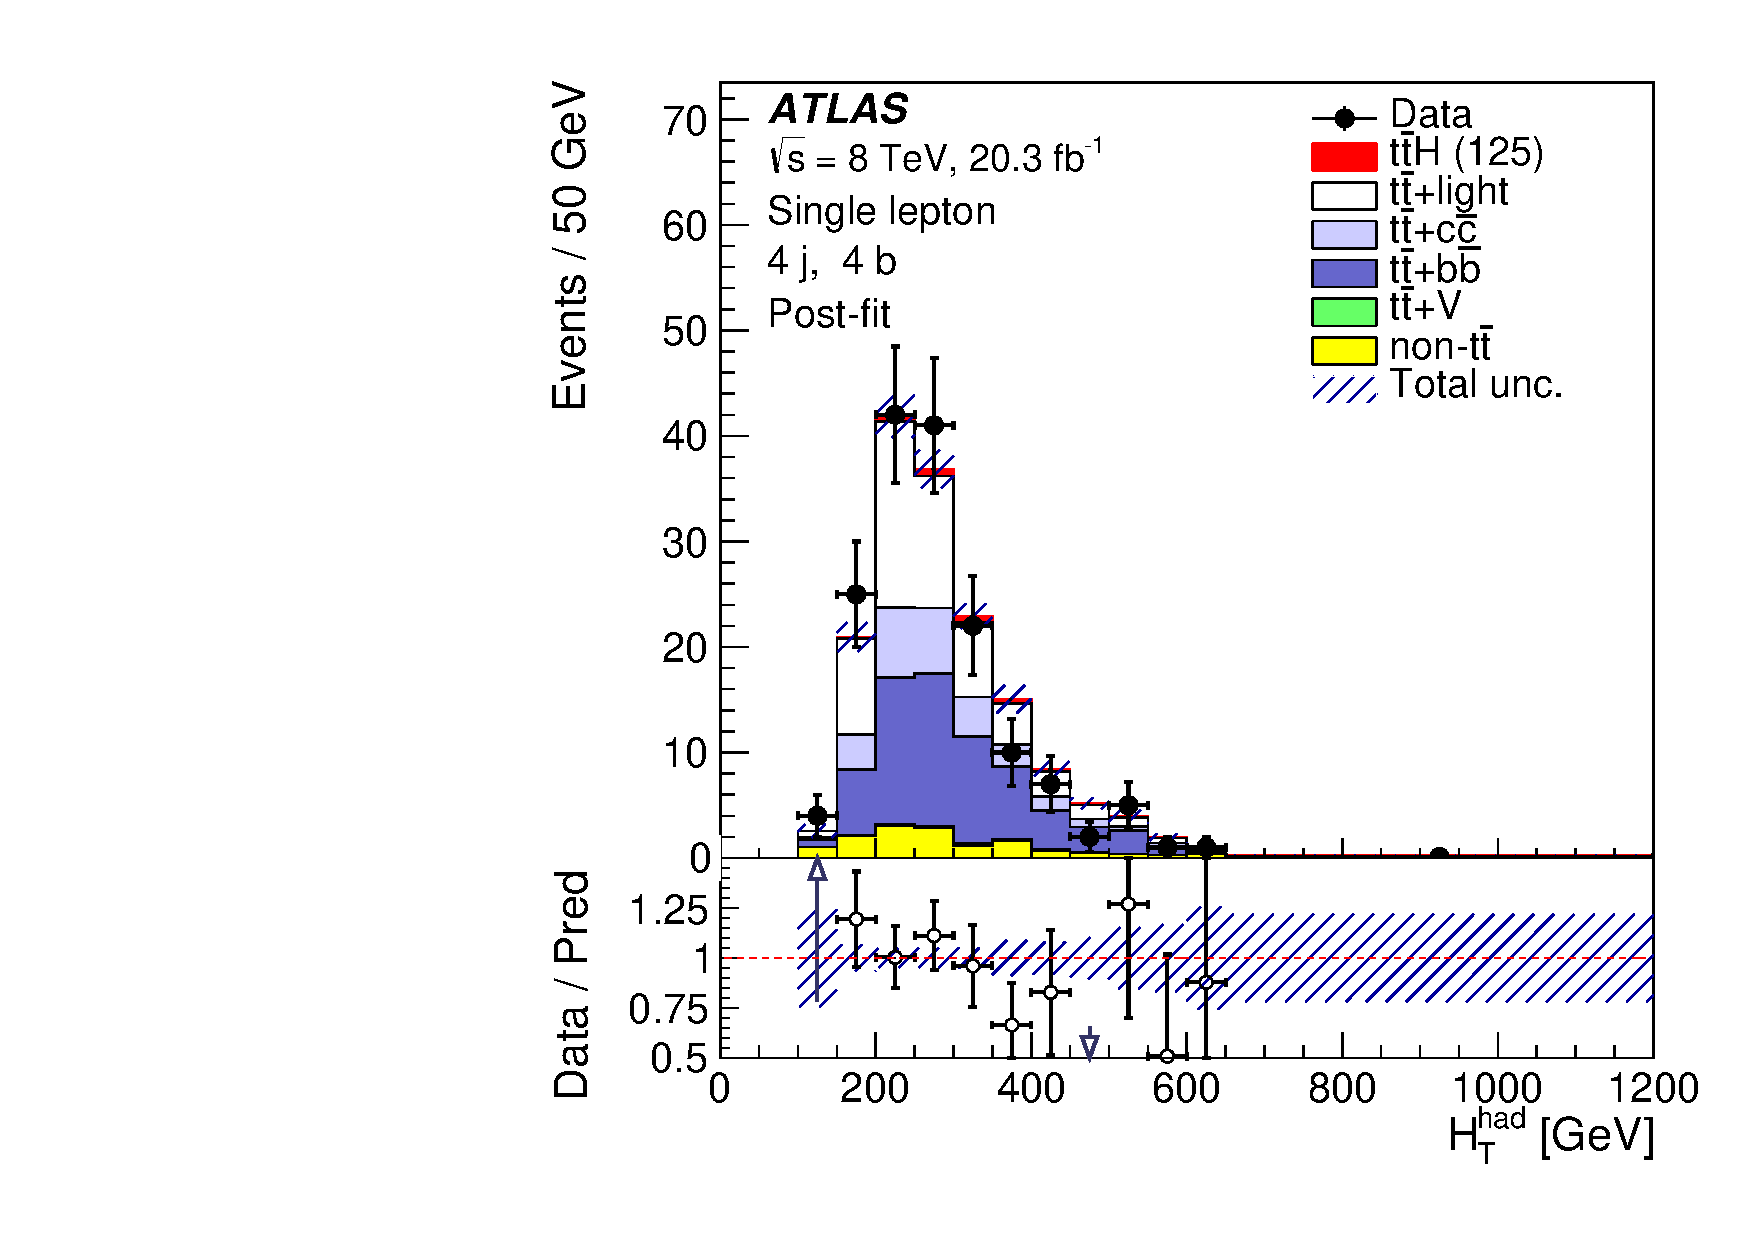
\includegraphics[width=\textwidth]{Analysis/Figures_ttH/HTHad_4jetex4btagin8TeV.pdf}
  \caption{}\end{subfigure}
  \begin{subfigure}{0.44\textwidth}
  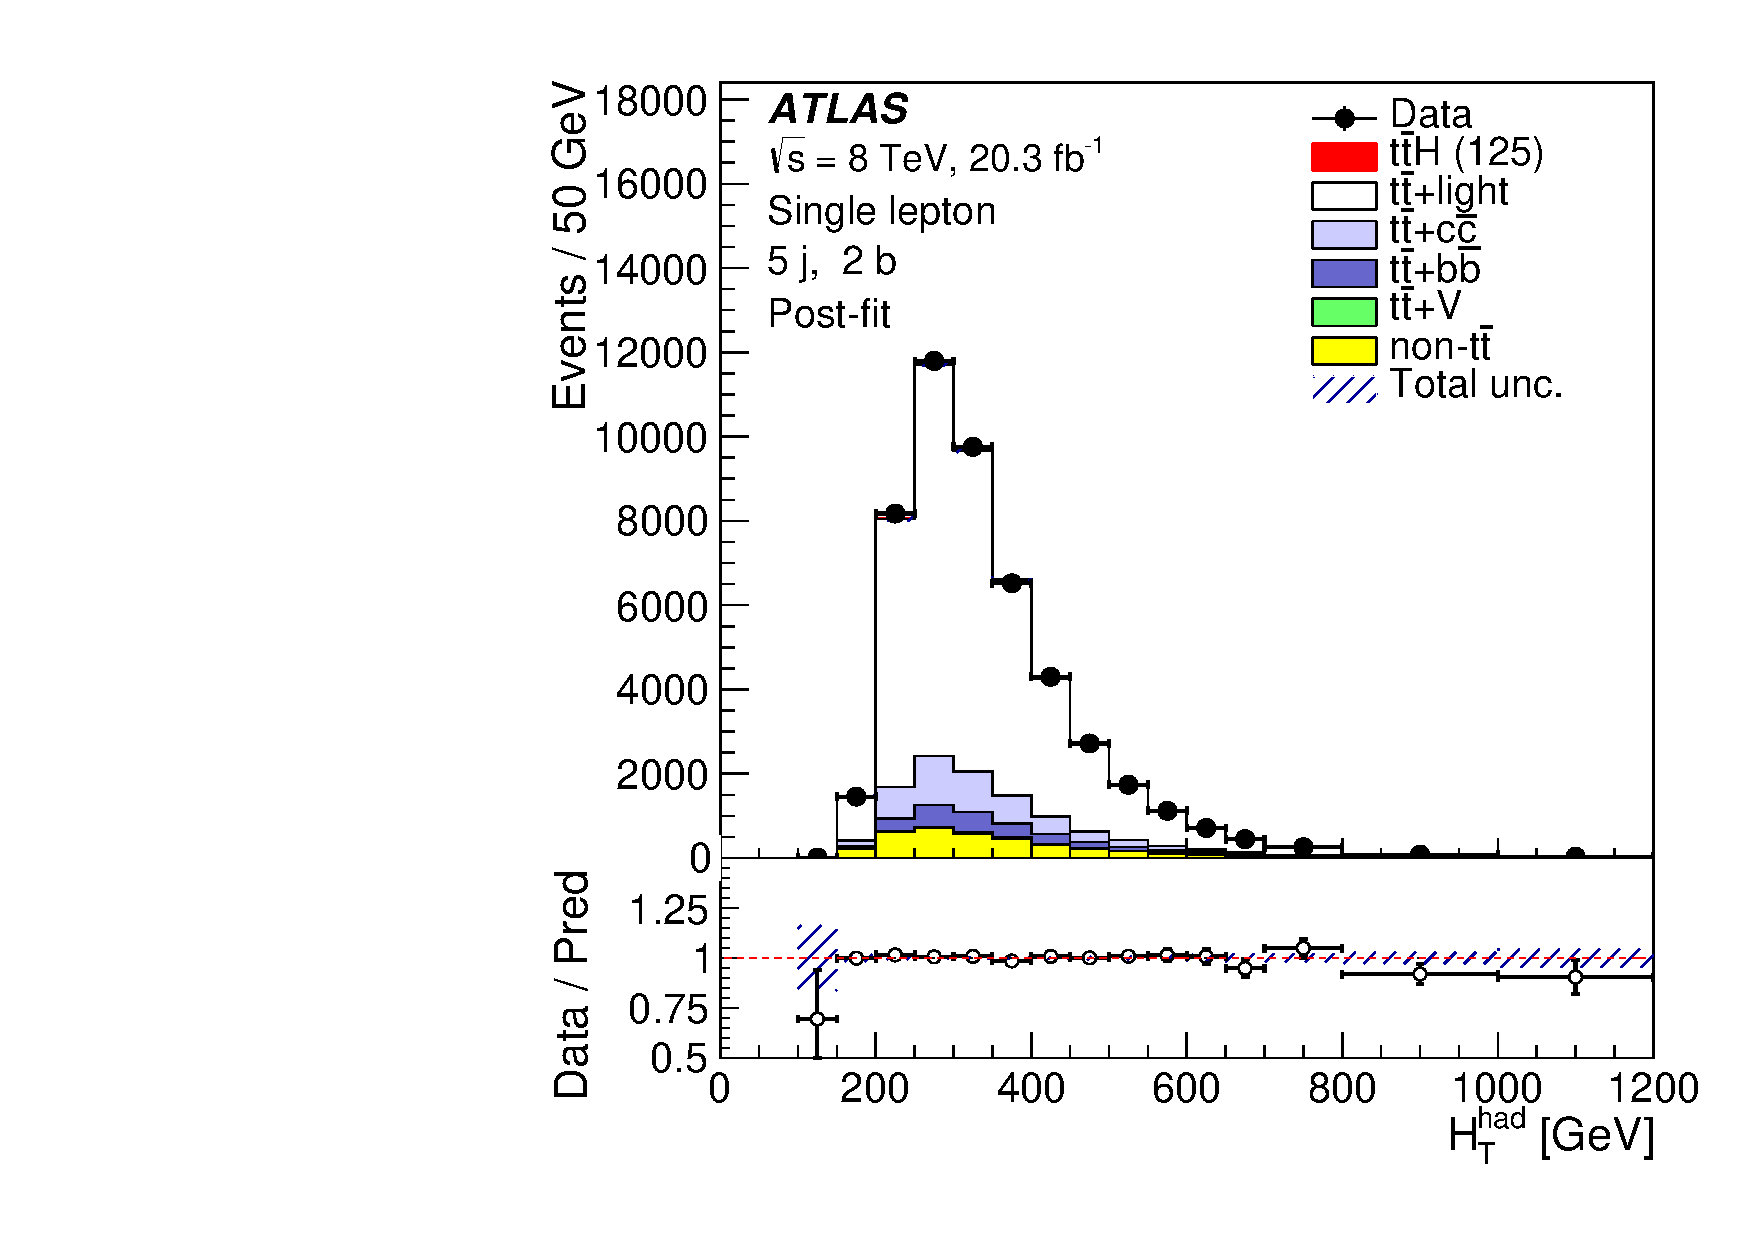
\includegraphics[width=\textwidth]{Analysis/Figures_ttH/HTHad_5jetex2btagex8TeV.pdf}
  \caption{}\end{subfigure}
  \begin{subfigure}{0.44\textwidth}
  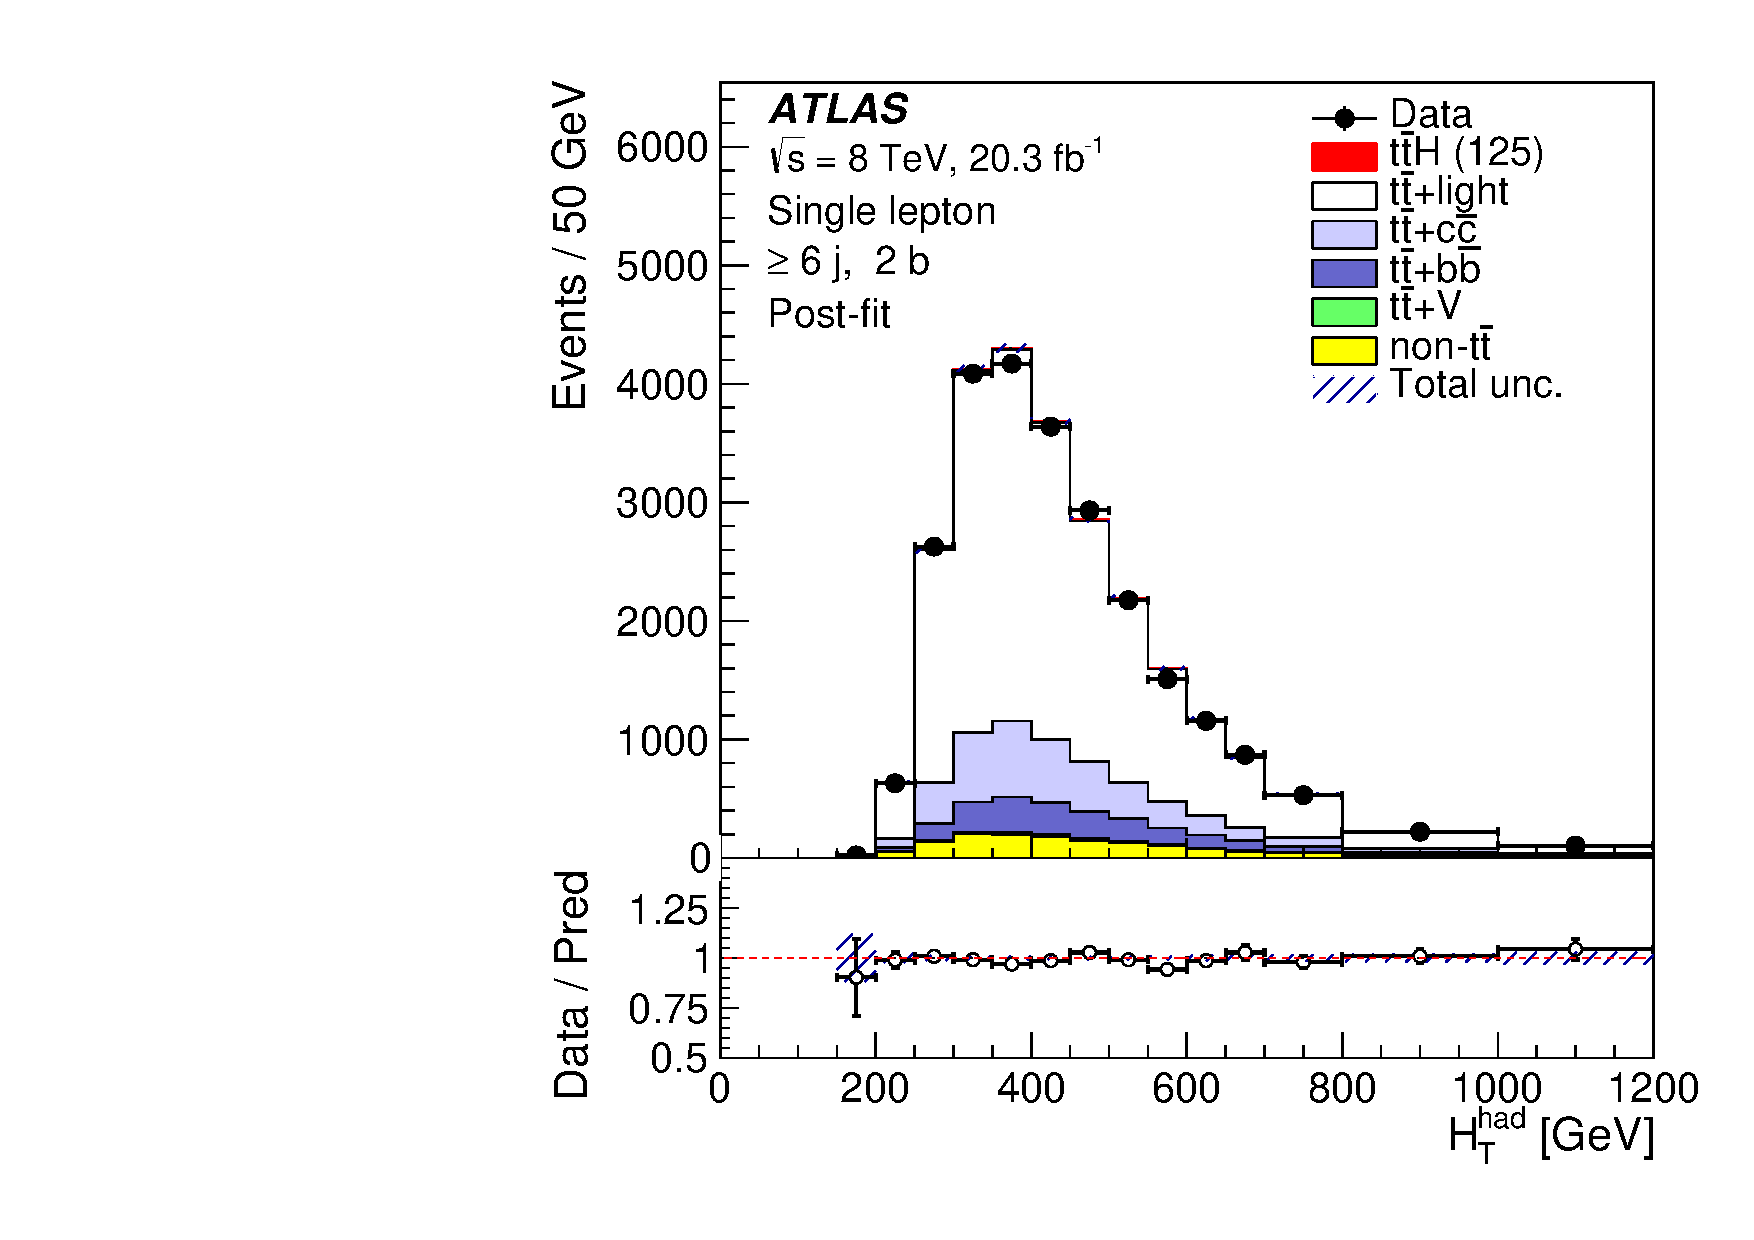
\includegraphics[width=\textwidth]{Analysis/Figures_ttH/HTHad_6jetin2btagex8TeV.pdf}
  \caption{}\end{subfigure}
  \caption{Comparison between data and prediction for the $\hthad$ distribution in the signal-depleted regions after the fit:
  (a) \fourtwo, (b) \fourthree, (c) \fourfour, (d) \fivetwo\ and (e) \sixtwo.
The hashed area represents the uncertainty on the background and the last bin in all figures contains the overflow. 
The \tth\ signal yield is normalized to the fitted $\mu$ and stacked on top of the background prediction.
}
  \label{fig:postfit_ttH_1}
\end{figure}

\begin{figure}[tpb!]
  \centering
  \begin{subfigure}{0.49\textwidth}
  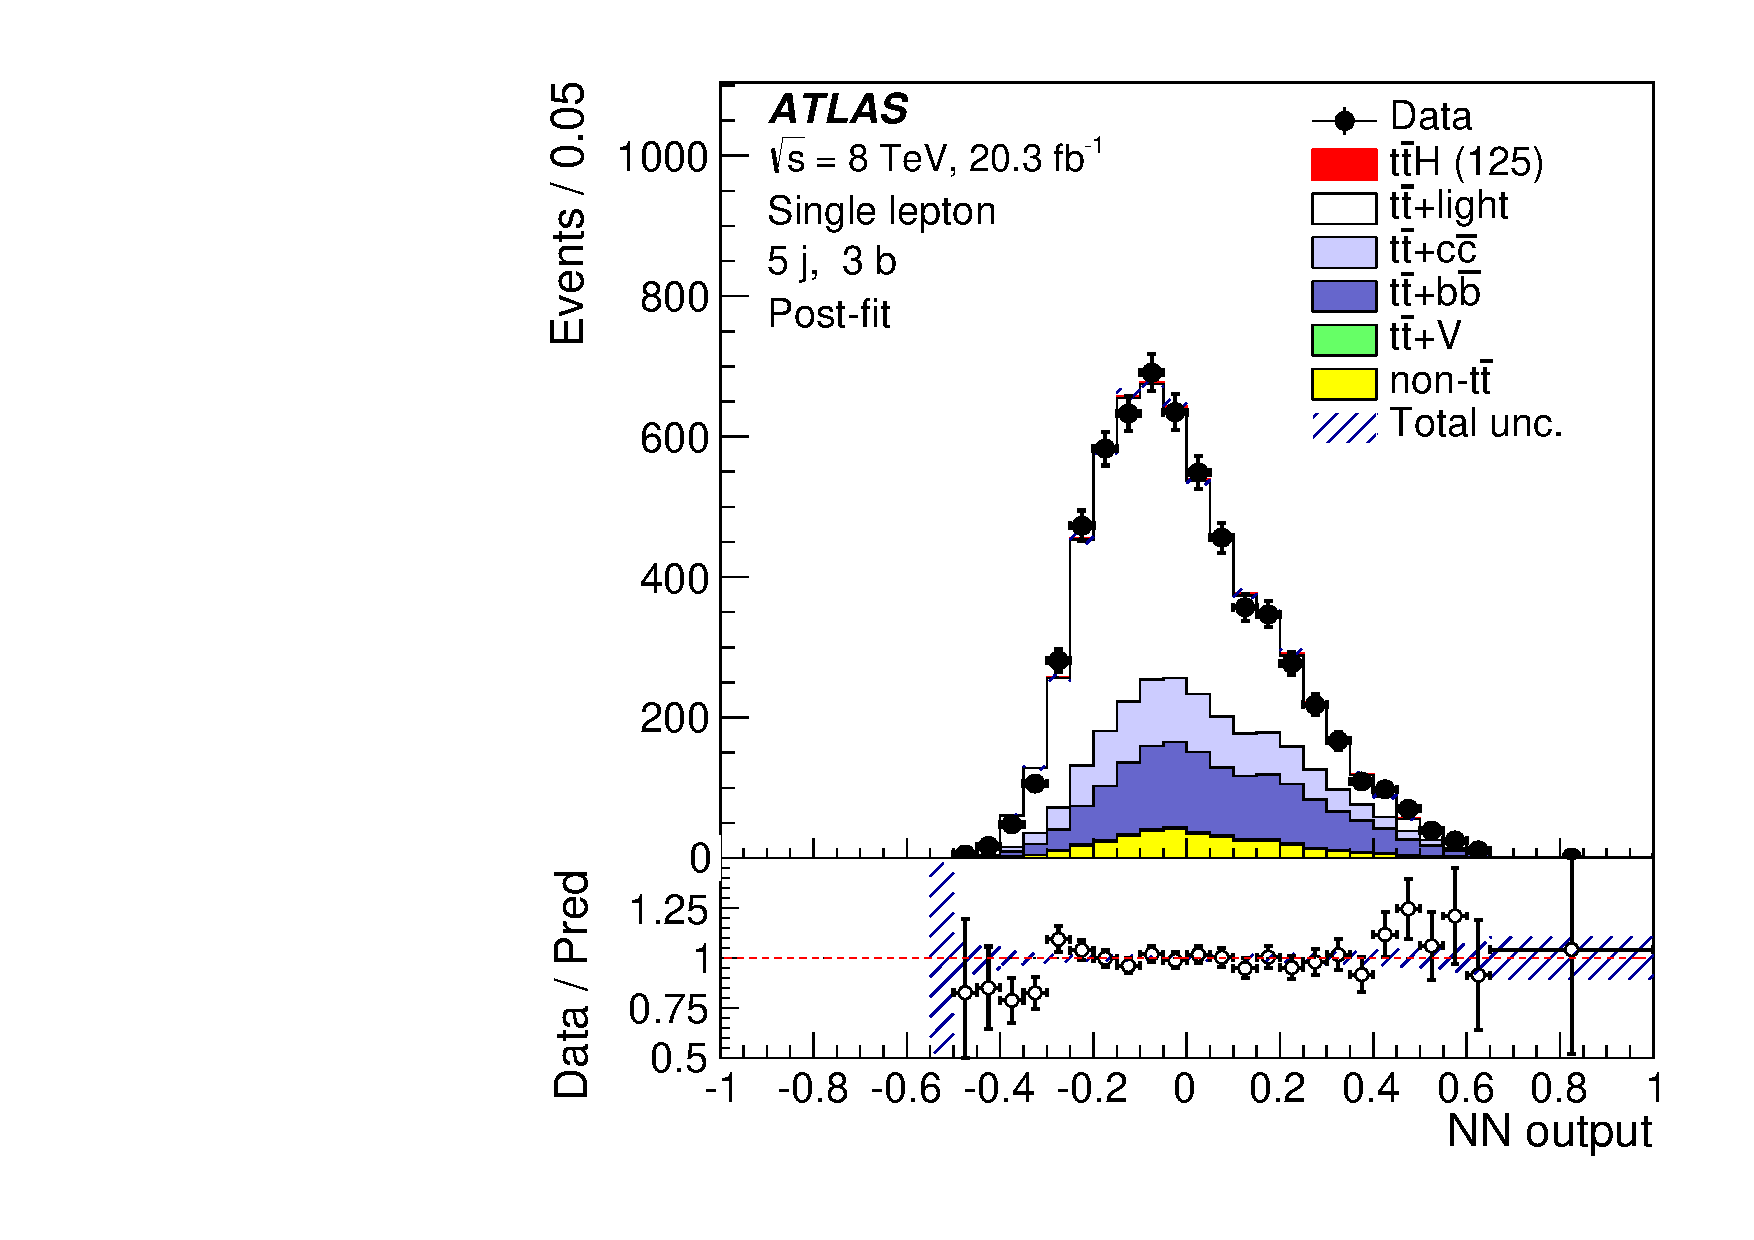
\includegraphics[width=\textwidth]{Analysis/Figures_ttH/NN_5jetex3btagex8TeV.pdf}
  \caption{}\end{subfigure}
  \begin{subfigure}{0.49\textwidth}
  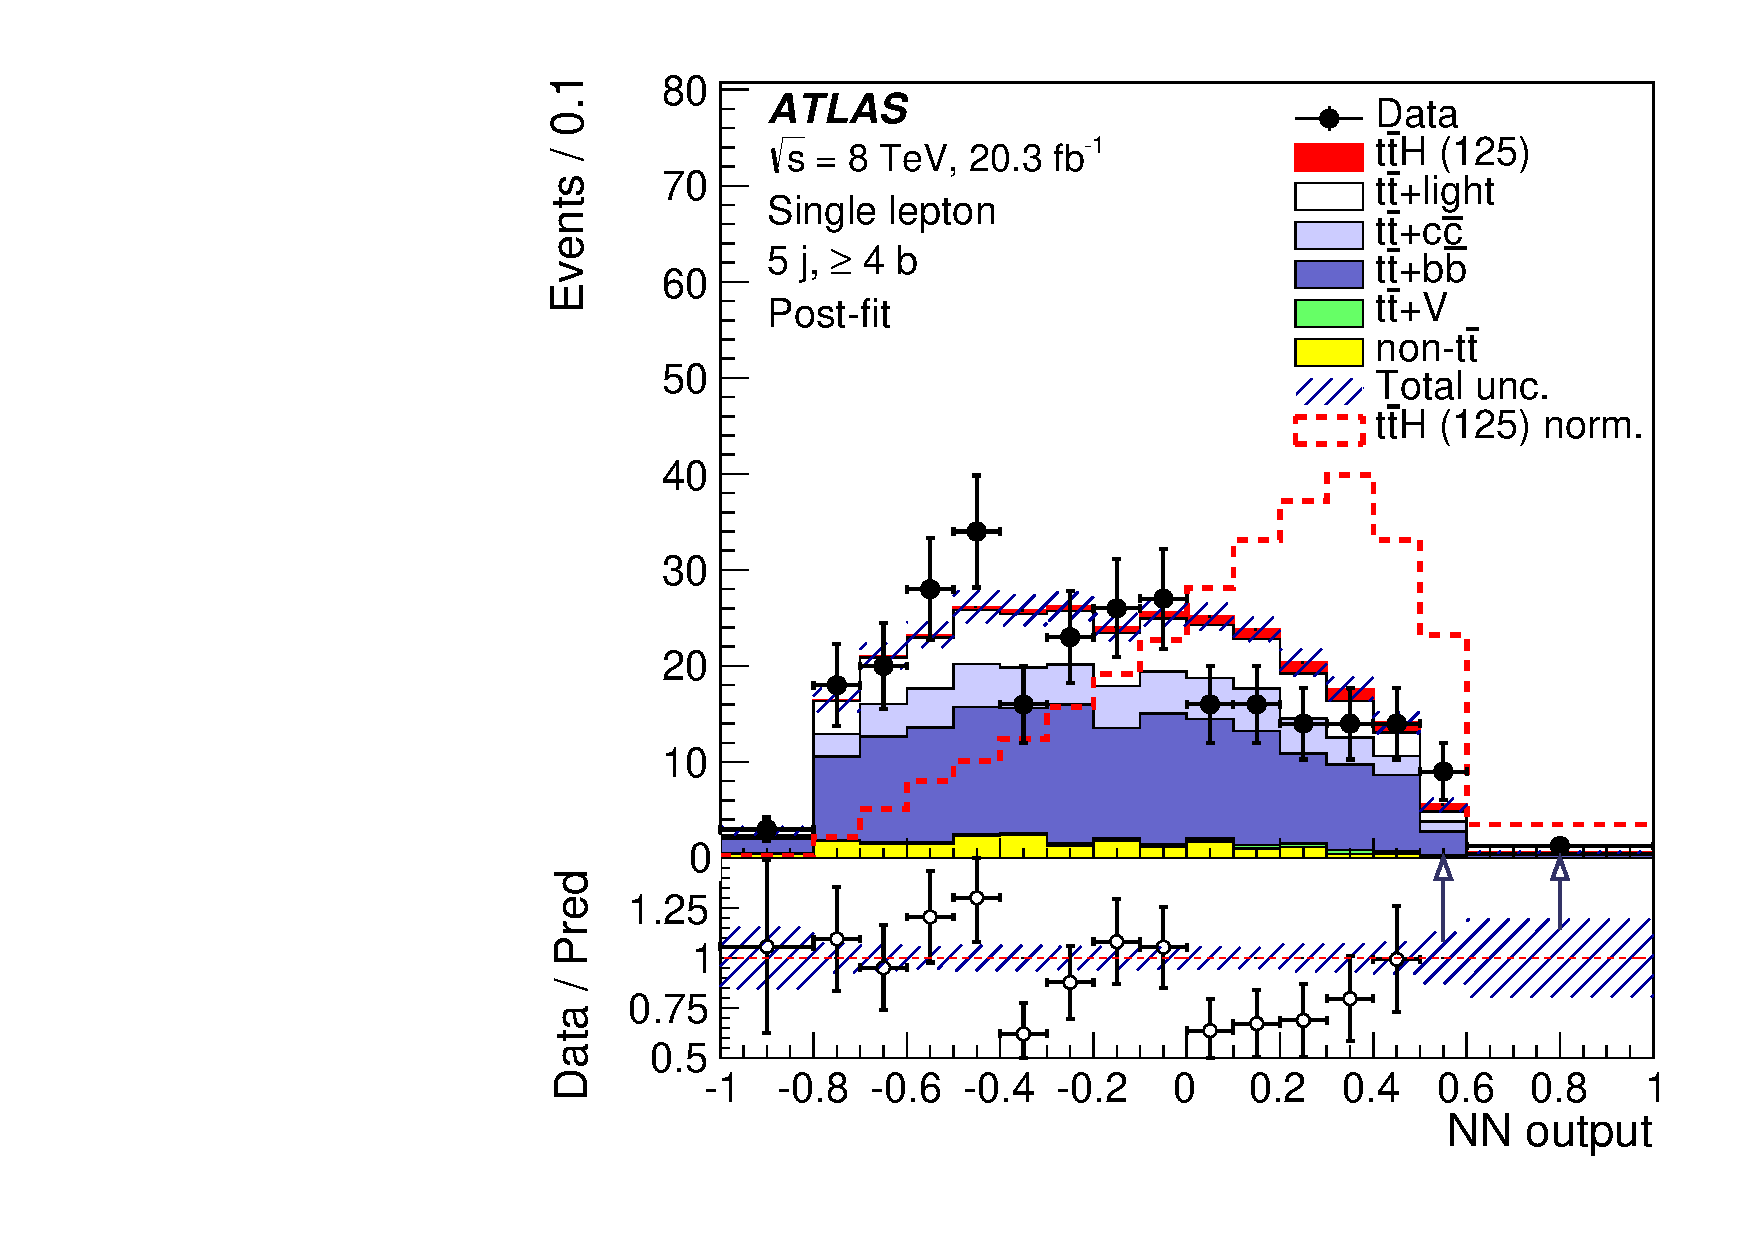
\includegraphics[width=\textwidth]{Analysis/Figures_ttH/NN_5jetex4btagin8TeV.pdf}
  \caption{}\end{subfigure}
  \begin{subfigure}{0.49\textwidth}
  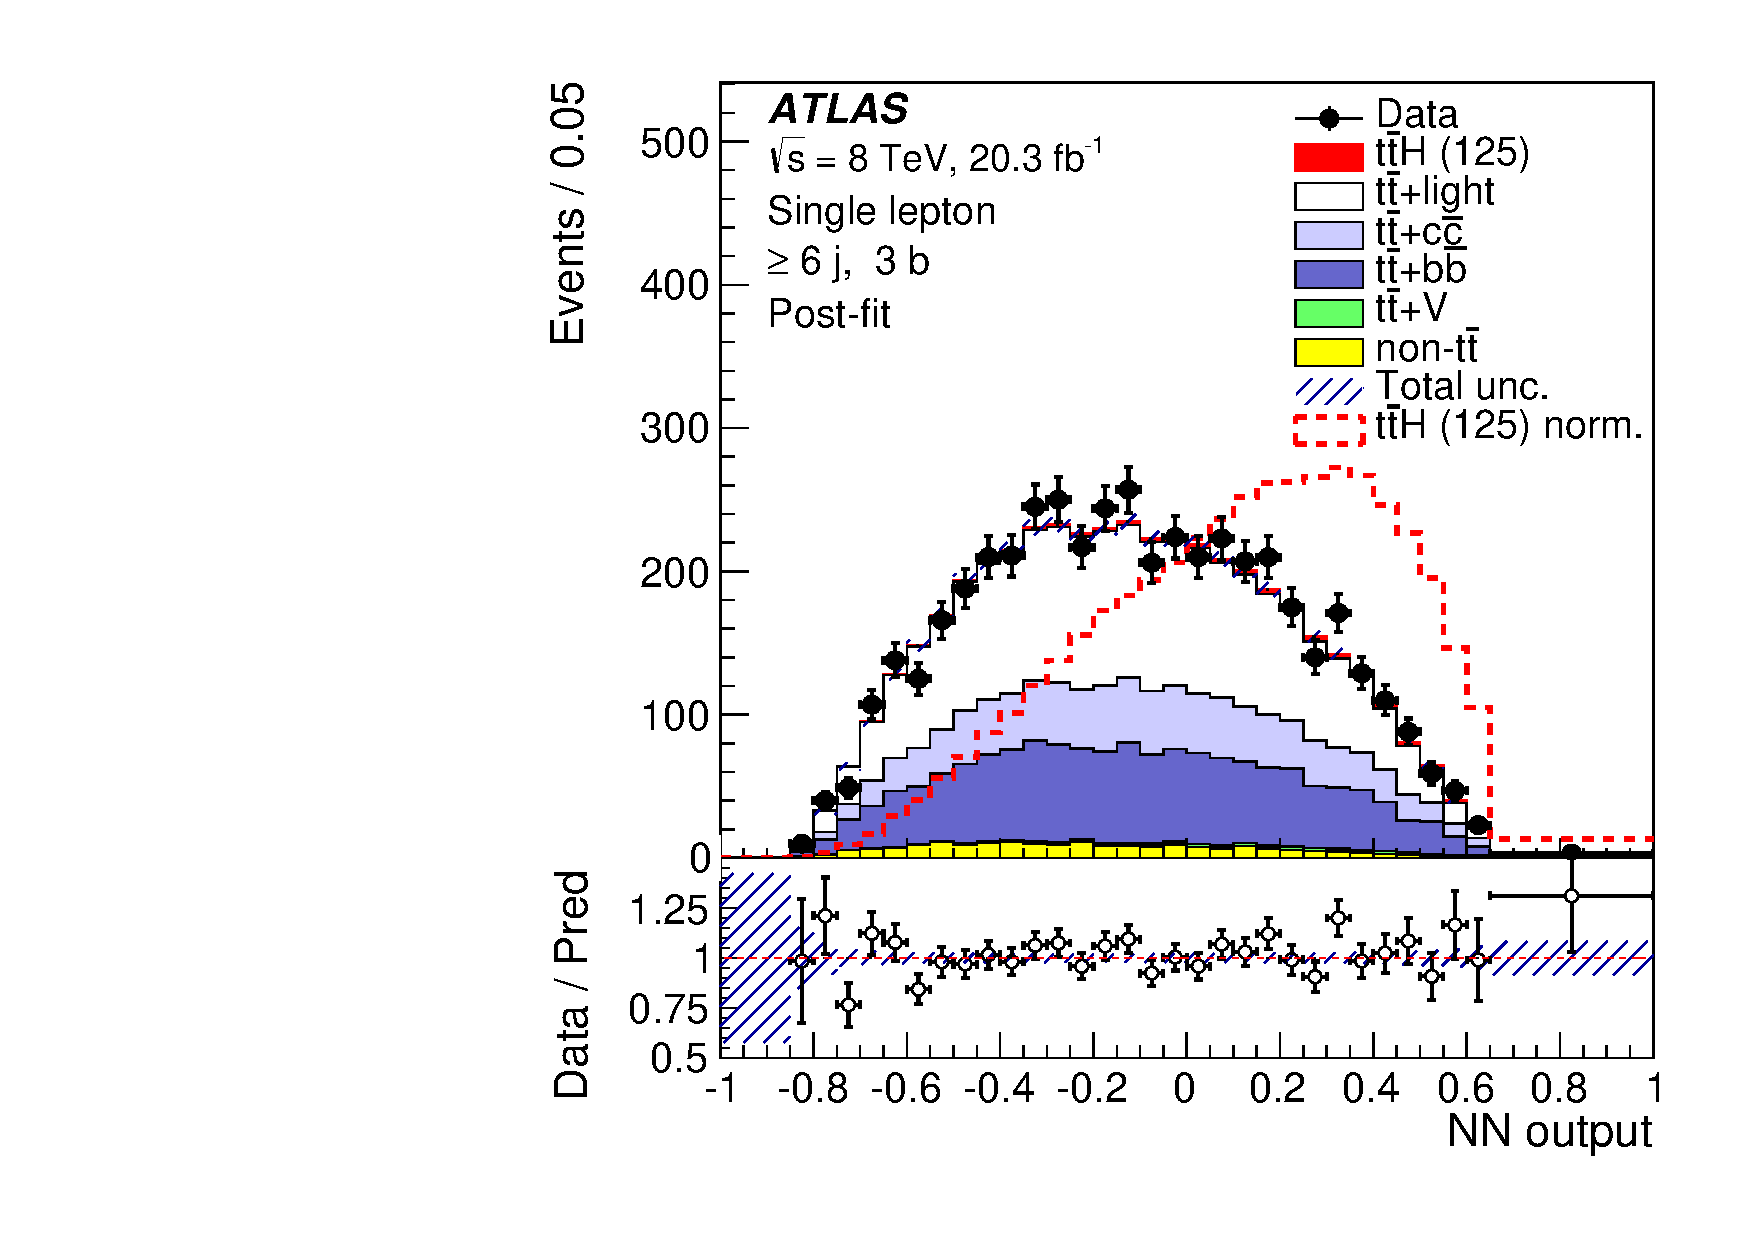
\includegraphics[width=\textwidth]{Analysis/Figures_ttH/NN_6jetin3btagex8TeV.pdf}
  \caption{}\end{subfigure}
  \begin{subfigure}{0.49\textwidth}
  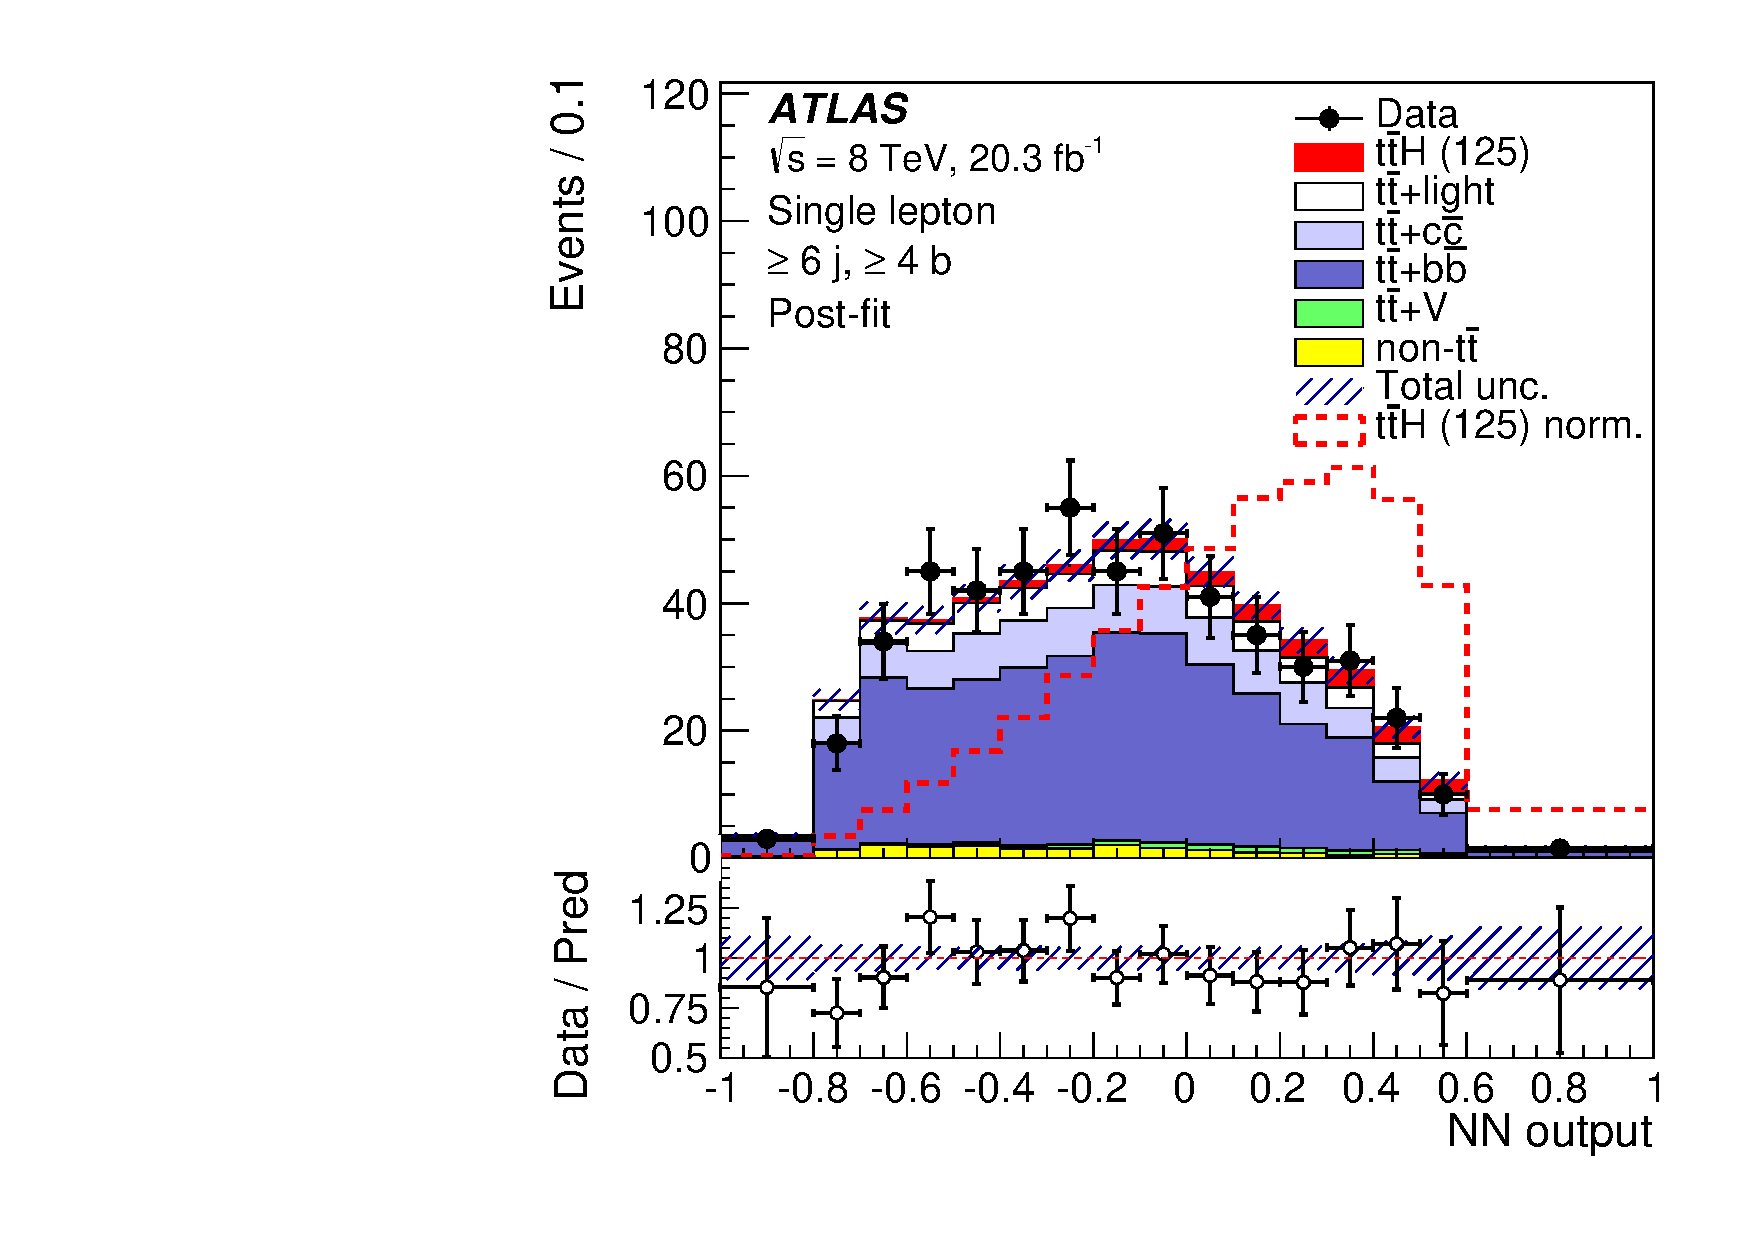
\includegraphics[width=\textwidth]{Analysis/Figures_ttH/NN_6jetin4btagin8TeV.pdf}
  \caption{}\end{subfigure}
  \caption{Comparison between data and prediction for the $NN$ distribution in the signal-rich regions and the \fivethree\ region after the fit:
  (a) \fivethree, (b) \fivefour, (c) \sixthree\ and (d) \sixfour.
The hashed area represents the uncertainty on the background and the last bin in all figures contains the overflow. 
The \tth\ signal yield is  normalized to the fitted $\mu$ (solid) and normalized to the total background prediction (hashed line) in order to compare the shape of the distributions.
}
  \label{fig:postfit_ttH_2}
\end{figure}

\begin{table}[tp!]
\begin{center}
\begin{tabular}{l*{3}{r@{$\,\pm\,$}r}}%
\hline\hline
 & \multicolumn{2}{c}{4 j, 2 b} & \multicolumn{2}{c}{4 j, 3 b} & \multicolumn{2}{c}{4 j, 4 b}\\
\hline
$t\bar{t}H$ (125) & \numRF{47.58}{2} & \numRF{34.91}{2} & \numRF{20.03}{2} & \numRF{14.69}{2} & \numRF{3.03}{2} & \numRF{2.23}{2}\\
$t\bar{t}+$ light & \numRF{78240.75}{2} & \numRF{1574.18}{2} & \numRF{6263.72}{2} & \numRF{161.34}{2} & \numRF{56.45}{2} & \numRF{4.71}{1}\\
$t\bar{t}+c\bar{c}$ & \numRF{6433.38}{2} & \numRF{1796.53}{2} & \numRF{845.05}{2} & \numRF{220.43}{2} & \numRF{25.54}{2} & \numRF{6.54}{1}\\
$t\bar{t}+b\bar{b}$ & \numRF{2475.84}{2} & \numRF{487.98}{2} & \numRF{969.03}{2} & \numRF{148.87}{2} & \numRF{62.51}{2} & \numRF{8.48}{1}\\
$W$+jets & \numRF{3654.81}{2} & \numRF{1116.58}{2} & \numRF{165.88}{2} & \numRF{51.34}{2} & \numRF{4.00}{2} & \numRF{1.24}{2}\\
$Z$+jets & \numRF{1058.08}{2} & \numRF{535.13}{2} & \numRF{49.12}{2} & \numRF{25.09}{2} & \numRF{1.06}{2} & \numRF{0.57}{1}\\
Single top & \numRF{4712.43}{2} & \numRF{322.17}{2} & \numRF{332.61}{2} & \numRF{28.10}{2} & \numRF{6.81}{2} & \numRF{0.73}{1}\\
Diboson & \numRF{215.89}{2} & \numRF{64.89}{2} & \numRF{11.33}{2} & \numRF{3.65}{1} & \numRF{0.28}{1} & \numRF{0.12}{1}\\
$t\bar{t}+V$ & \numRF{120.03}{2} & \numRF{37.66}{2} & \numRF{15.84}{2} & \numRF{4.92}{1} & \numRF{0.94}{1} & \numRF{0.29}{1}\\
Multijet & \numRF{1082.01}{2} & \numRF{367.87}{2} & \numRF{78.36}{2} & \numRF{26.20}{2} & \numRF{2.59}{2} & \numRF{0.99}{1}\\
\hline
Total & \numRF{98040.79}{2} & \numRF{336.60}{2}   & \numRF{8750.98}{2} & \numRF{81.58}{2}   & \numRF{163.21}{2} & \numRF{5.63}{1}  \\
\hline
Data & \multicolumn{2}{l}{\num{98049}}  & \multicolumn{2}{l}{\num{8752}}  & \multicolumn{2}{l}{\num{161}} \\
\hline\hline     \\
\end{tabular}

\begin{tabular}{l*{3}{r@{$\,\pm\,$}r}}%
\hline\hline
 & \multicolumn{2}{c}{5 j, 2 b} & \multicolumn{2}{c}{5 j, 3 b} & \multicolumn{2}{c}{5 j, $\geq$ 4 b}\\
\hline
$t\bar{t}H$ (125) & \numRF{60.39}{2} & \numRF{44.18}{2} & \numRF{33.72}{2} & \numRF{24.66}{2} & \numRF{9.42}{2} & \numRF{6.89}{2}\\
$t\bar{t}+$ light & \numRF{38387.98}{2} & \numRF{1046.42}{2} & \numRF{3614.11}{2} & \numRF{116.75}{2} & \numRF{65.28}{2} & \numRF{5.59}{1}\\
$t\bar{t}+c\bar{c}$ & \numRF{4801.21}{2} & \numRF{1203.63}{2} & \numRF{934.58}{2} & \numRF{230.20}{2} & \numRF{50.70}{2} & \numRF{12.47}{2}\\
$t\bar{t}+b\bar{b}$ & \numRF{2376.48}{2} & \numRF{364.28}{2} & \numRF{1260.77}{2} & \numRF{176.75}{2} & \numRF{154.69}{2} & \numRF{19.93}{2}\\
$W$+jets & \numRF{1208.16}{2} & \numRF{424.84}{2} & \numRF{86.55}{2} & \numRF{30.69}{2} & \numRF{4.04}{2} & \numRF{1.45}{2}\\
$Z$+jets & \numRF{367.88}{2} & \numRF{204.43}{2} & \numRF{27.88}{2} & \numRF{15.59}{2} & \numRF{1.40}{2} & \numRF{0.80}{1}\\
Single top & \numRF{1726.09}{2} & \numRF{152.89}{2} & \numRF{185.02}{2} & \numRF{17.78}{2} & \numRF{8.17}{2} & \numRF{0.66}{1}\\
Diboson & \numRF{93.76}{2} & \numRF{35.15}{2} & \numRF{7.96}{2} & \numRF{3.14}{2} & \numRF{0.45}{1} & \numRF{0.19}{1}\\
$t\bar{t}+V$ & \numRF{137.94}{2} & \numRF{43.15}{2} & \numRF{26.11}{2} & \numRF{8.06}{1} & \numRF{3.19}{2} & \numRF{0.98}{1}\\
Multijet & \numRF{342.54}{2} & \numRF{112.21}{2} & \numRF{43.52}{2} & \numRF{15.83}{2} & \numRF{5.73}{2} & \numRF{2.20}{2}\\
\hline
Total & \numRF{49502.44}{2} & \numRF{221.76}{2}   & \numRF{6220.20}{2} & \numRF{53.55}{2}   & \numRF{303.08}{2} & \numRF{9.54}{1}  \\
\hline
Data & \multicolumn{2}{l}{\num{49699}}  & \multicolumn{2}{l}{\num{6199}}  & \multicolumn{2}{l}{\num{286}} \\
\hline\hline     \\
\end{tabular}

\begin{tabular}{l*{3}{r@{$\,\pm\,$}r}}%
\hline\hline
 & \multicolumn{2}{c}{$\geq$ 6 j, 2 b} & \multicolumn{2}{c}{$\geq$ 6 j, 3 b} & \multicolumn{2}{c}{$\geq$ 6 j, $\geq$ 4 b}\\
\hline
$t\bar{t}H$ (125) & \numRF{88.96}{2} & \numRF{65.04}{2} & \numRF{57.00}{2} & \numRF{41.64}{2} & \numRF{23.56}{2} & \numRF{17.19}{2}\\
$t\bar{t}+$ light & \numRF{18938.70}{2} & \numRF{704.70}{2} & \numRF{2077.28}{2} & \numRF{87.41}{2} & \numRF{57.88}{2} & \numRF{5.26}{1}\\
$t\bar{t}+c\bar{c}$ & \numRF{3733.31}{2} & \numRF{889.24}{2} & \numRF{888.02}{2} & \numRF{210.88}{2} & \numRF{85.40}{2} & \numRF{20.57}{2}\\
$t\bar{t}+b\bar{b}$ & \numRF{1980.03}{2} & \numRF{311.13}{2} & \numRF{1357.44}{2} & \numRF{187.71}{2} & \numRF{330.81}{2} & \numRF{37.31}{2}\\
$W$+jets & \numRF{454.72}{2} & \numRF{173.62}{2} & \numRF{50.73}{2} & \numRF{19.42}{2} & \numRF{4.43}{2} & \numRF{1.85}{2}\\
$Z$+jets & \numRF{151.74}{2} & \numRF{86.28}{2} & \numRF{15.55}{2} & \numRF{8.89}{1} & \numRF{1.22}{2} & \numRF{0.70}{1}\\
Single top & \numRF{734.34}{2} & \numRF{83.37}{2} & \numRF{110.67}{2} & \numRF{13.91}{2} & \numRF{11.44}{2} & \numRF{1.55}{1}\\
Diboson & \numRF{44.67}{2} & \numRF{19.76}{2} & \numRF{5.58}{2} & \numRF{2.57}{2} & \numRF{0.53}{1} & \numRF{0.23}{1}\\
$t\bar{t}+V$ & \numRF{165.88}{2} & \numRF{51.54}{2} & \numRF{42.28}{2} & \numRF{12.86}{2} & \numRF{8.23}{2} & \numRF{2.51}{2}\\
Multijet & \numRF{116.90}{2} & \numRF{40.67}{2} & \numRF{13.78}{2} & \numRF{5.25}{1} & \numRF{1.13}{2} & \numRF{0.51}{1}\\
\hline
Total & \numRF{26409.24}{2} & \numRF{160.08}{2}   & \numRF{4618.33}{2} & \numRF{54.65}{2}   & \numRF{524.62}{2} & \numRF{17.91}{2}  \\
\hline
Data & \multicolumn{2}{l}{\num{26185}}  & \multicolumn{2}{l}{\num{4701}}  & \multicolumn{2}{l}{\num{516}} \\
\hline\hline     \\
\end{tabular}

%
\end{center}
\vspace{-0.5cm}
\caption{Post-fit event yields under the 
signal-plus-background hypothesis
for signal, backgrounds and data in each of the analysis regions.
The
quoted uncertainties are the sum in quadrature of statistical and
systematic uncertainties on the yields, computed taking into
account correlations among nuisance parameters and among processes.
}
\label{tab:Postfit_EventsTable_lj}
\end{table}
 


A good agreement is found between data and prediction in all channels. The good performance of the fit can further be validated through comparison between data and total prediction for other kinematic distributions. Pre-fit and post-fit distributions for different distributions can be found in appendix~\ref{app:DataMC_validation_ttH}. 
The agreement for other kinematic distributions not used in the fit is also improved
after the fit, giving confidence in the overall procedure.

Given the regions considered in the fit, some of the NPs are expected to be constrained by the data and possibly pulled, 
in particular those associated with large uncertainties on $t\bar{t}$ modeling. 
The most relevant pulls and constrains are discussed in the following:
\begin{itemize}
  \item JetModel1: the largest eigenvector after diagonalization of the modeling uncertainties in the in-situ calibration of the jet energy scale.
    The effect of this uncertainty is shown in figure~\ref{fig:control_JetModel1} for the \ttbar+light jets process in the \fourtwo\ region. It produces a $\sim \unit[4]{\%}$ effect in the bulk of the distribution, and up to $\sim \unit[10]{\%}$ in the lower tail. The high data statistics in this region, of up to 30000 events in one bin, doesn't support such big variations and therefore the uncertainty is constrained. %Main contribution to modeling comes from full difference between Pythia and Alpgen+Herwig in modeling Z-pT
  \item JetFlavComp: the uncertainty on the jet flavor composition. Since the jet energy response is different for quark-initiated jets than for gluon-initiated jets~\cite{Aad:2014gea}, analyses with a different flavor fraction than the sample used to derive the jet energy scale calibration are affected by this uncertainty. The effect of the negative pull is an increase in the low tail of the distribution, as shown in figure~\ref{fig:control_JetFlavComp}, which corrects the disagreement at low $\hthad$ in the \fourtwo\ region. It has been checked that the pull disappears when removing this region from the fit and, given that this systematic uncertainty is not correlated with the signal strength, this pull is not problematic. 
  \item JVF: the jet vertex fraction uncertainty is constrained to about half of its pre-fit effect. The uncertainty was assessed by changing the JVF cut as to cover data/MC differences in a sample with one single jet. In this analysis the simultaneous variation of the JVF cut for all the jets in the event produces a large variation that is not supported by data and is therefore constrained.
  \item JER: the jet energy resolution uncertainty is constrained to about half of its pre-fit effect. This constrain originates from the conservative approach used to estimate the uncertainty for low-\pt\ jets as mentioned in section~\ref{subsec:JER}. Since the bulk of the contribution originates from low-\pt\ jets this uncertainty can be reduced with the selected data sample. The effect of the jet energy resolution on the \ttbar+light-jets sample in the \fourtwo\ region is shown in figure~\ref{fig:control_JER}.
  \item $c$-tagging eigenvector 3: this corresponds to the largest eigenvector after diagonalization of the $c$-tagging uncertainties. The region \fourthree\ is very sensitive to the $c$-tagging uncertainty (see figure~\ref{fig:control_Ctag3}) since its main contribution comes from \ttbar\ events where a charm quark from the hadronic $W$ decay is tagged. The high statistics of this region allows the reduction of the uncertainty, which was derived on a sample of $D^{*+}$ events. The use of $c$-quarks from $W$ decays in \ttbar\ events is in fact a method that is in consideration for future $c$-tag calibrations.
  \item $b$-tagging eigenvector 5: this uncertainty corresponds to the largest eigenvector after diagonalization of the $b$-tagging uncertainties. It introduces a $\sim \unit[2]{\%}$ variation per $b$-tagged jet that is amplified to $\sim \unit[8]{\%}$ in the 4 $b$-tag regions. The simultaneous fit of different $b$-tag multiplicities allows reducing this uncertainty.
  \item QCD electron: the \unit[50]{\%} normalization uncertainty on the electron component of the multijet prediction. This pull has been traced to be originated from individual bins in the very low tail of the $\hthad$ distributions. Introducing cuts on \met\ or \mtw\ reduces the multijet component and doesn't alter significantly the result of the fit, however it reduces the sensitivity of the search. Given the negligible contribution of the multijet background and that it has no impact on the signal this pull is not considered problematic.
  \item ttbar DataRw-IFSR: the variation on the \ttbar\ reweighting due to the systematic uncertainty associated to initial- and final-state radiation in the differential \xsec\ measurement. Out of the nine components of the reweighting this uncertainty has the largest effect on the \ttbarpt\ spectrum, which propagates to the reconstructed jet multiplicity. This variation is not supported by the data and can be constrained. This constraint is in fact expected since the differential \xsec\ measurement is performed with the 7 \tev, which has a factor of four less statistics than the dataset used for this analysis. Other components of the \ttbar\ reweighting such as the choice of MC generator or the fragmentation model are also slightly constrained. The impact of this systematic uncertainty on the \ttbar+light-jets sample in the \fourtwo\ region is shown in figure~\ref{fig:control_IFSR}.
  \item ttbar PartonShower: the three NPs related to the choice of fragmentation model are pulled and/or constrained and deserve further attention. The NP affecting \ttbar+light jets is heavily constrained and fitted at its nominal value. The fitted value indicates that data supports the prediction of \PP. The prediction of \powheg+\herwig\ is in disagreement with data in the high-statistics channels and, since the full difference to \PP\ is taken as systematic uncertainty, the fit constrains the allowed variation to a smaller range. The effect on the \ttbar+light-jets sample in the \sixtwo\ region is shown in figure~\ref{fig:control_PS}.

    The NP related to \ttbb\ is in agreement with the nominal prediction, indicating that NLO prediction of \ShOL\ agrees with data. The effect of the fragmentation uncertainty is again too large and data can constrain this systematic uncertainty to a fraction of its pre-fit value.

    The pull on \ttcc\ is difficult to study since there is no NLO prediction to compare to and both predictions, \PP\ or \powheg+\herwig\, could be equally valid. The only anecdotal evidence supporting this pull is that the \ttC\ component in \powheg+\herwig\ is \unit[40]{\%} higher than in \PP, thus the pull towards \powheg+\herwig\ would introduce the same effect as the leading correction on the \ttB\ component, where the NLO prediction is observed to be \unit[40]{\%} higher than in \PP.
  \item ttbb normalization: the normalization of the \ttbb\ component is fitted to a value $\sim \unit[30]{\%}$ higher than its nominal prediction, and the uncertainty is reduced from the very conservative \unit[50]{\%} to \unit[20]{\%}. The data statistics in the \sixfour\ region allows reducing the uncertainty, therefore improving the sensitivity of the search. 

    The normalization uncertainty of the \ttcc\ background is also reduced, although to a smaller extent since there is no region where it is the dominant background.
\end{itemize}

\begin{figure}[tpb!]
  \centering
  \begin{subfigure}{0.47\textwidth}
     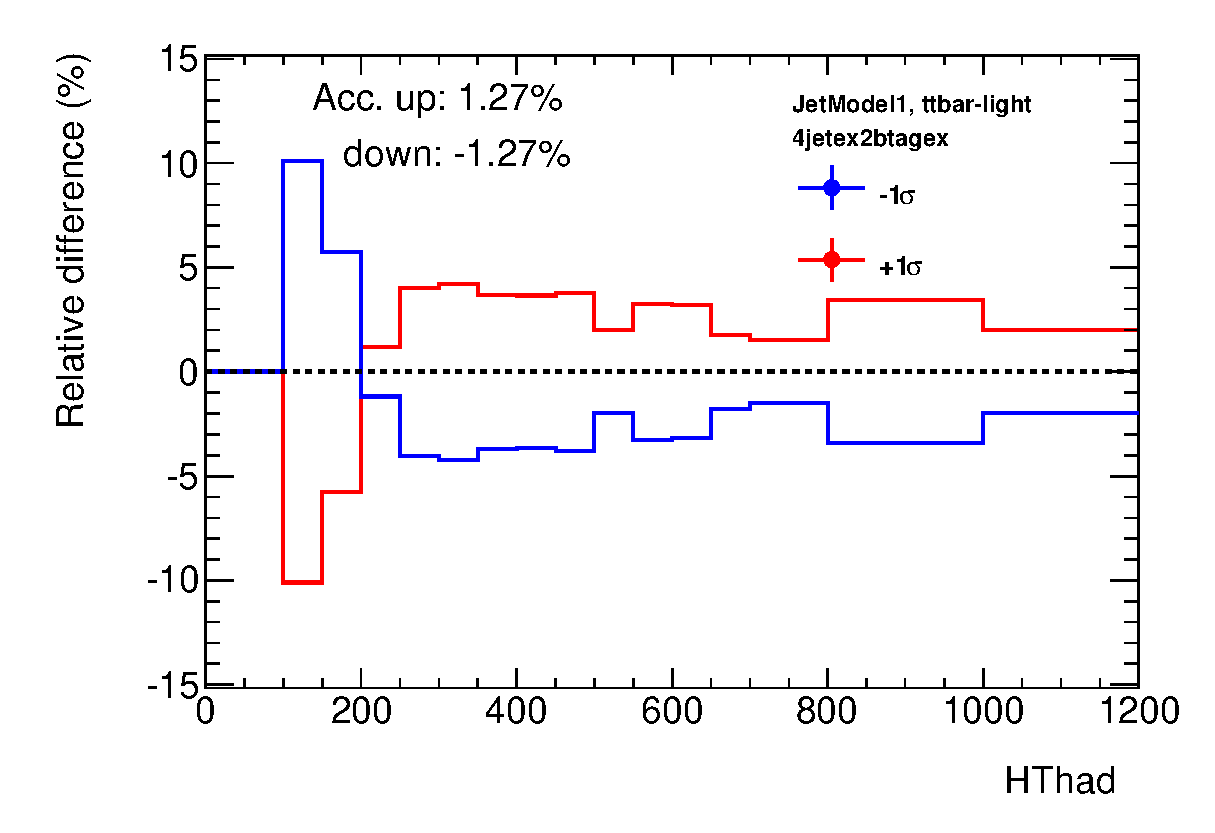
\includegraphics[width=\textwidth]{Analysis/Figures_ttH/ControlPlots/4jetex2btagex_ttbar-light_JetModel1.eps}
  \caption{} \label{fig:control_JetModel1}
  \end{subfigure}
  \begin{subfigure}{0.47\textwidth}
     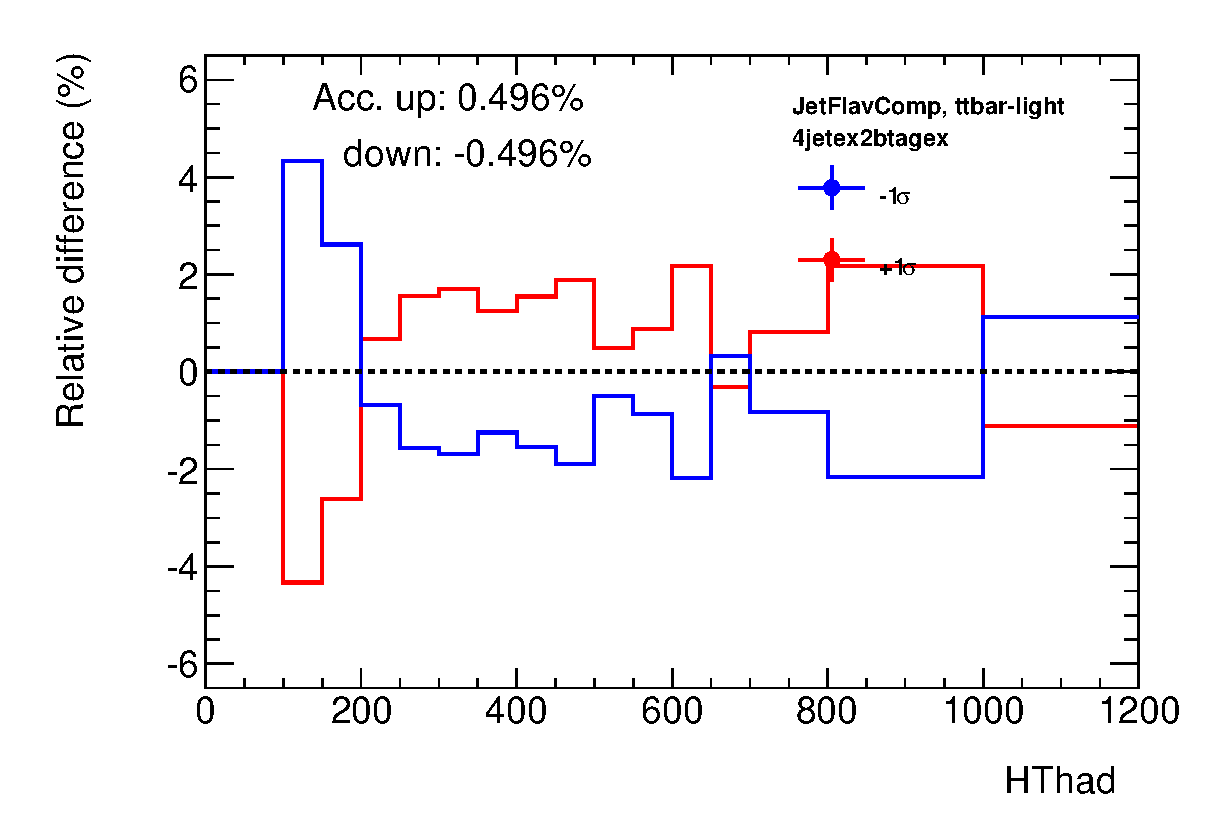
\includegraphics[width=\textwidth]{Analysis/Figures_ttH/ControlPlots/4jetex2btagex_ttbar-light_JetFlavComp.eps}
  \caption{} \label{fig:control_JetFlavComp}
  \end{subfigure} 
  \\
  \begin{subfigure}{0.47\textwidth}
     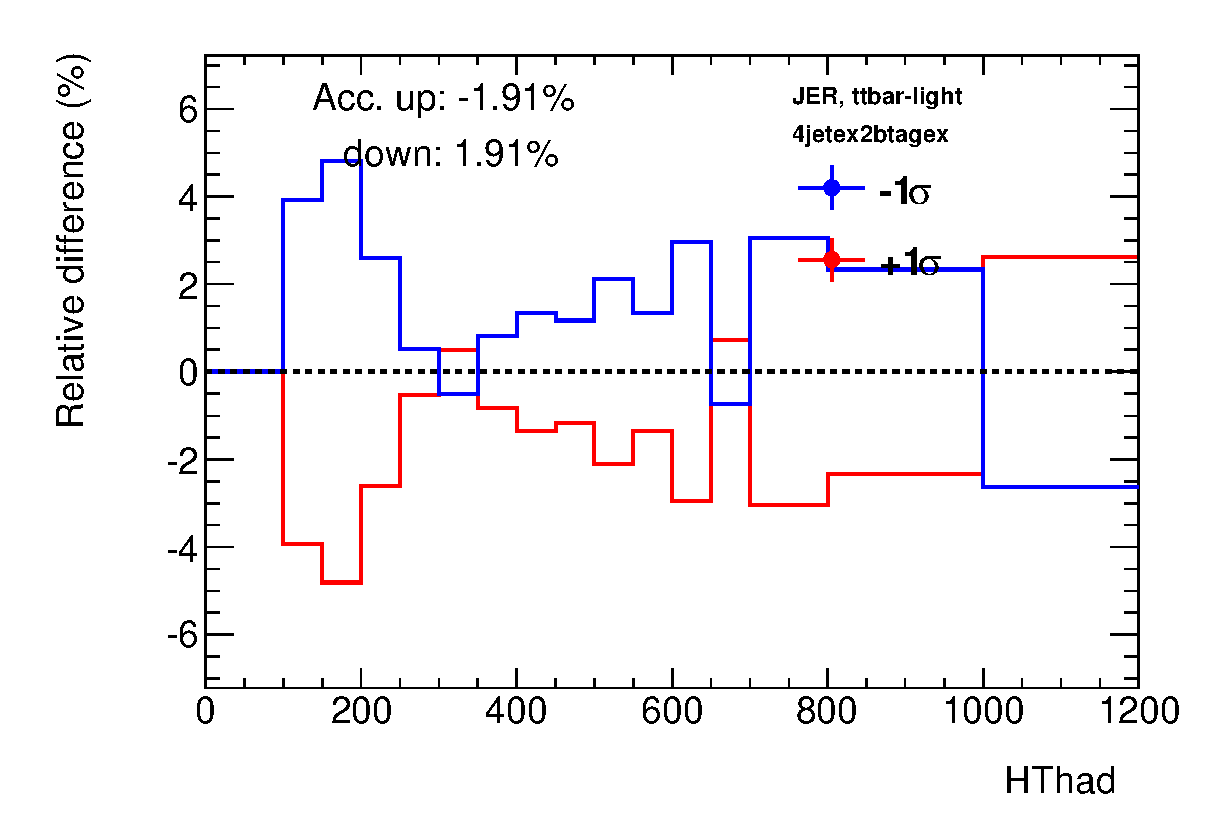
\includegraphics[width=\textwidth]{Analysis/Figures_ttH/ControlPlots/4jetex2btagex_ttbar-light_JER.eps}
     \caption{} \label{fig:control_JER}
  \end{subfigure}
  \begin{subfigure}{0.47\textwidth}
     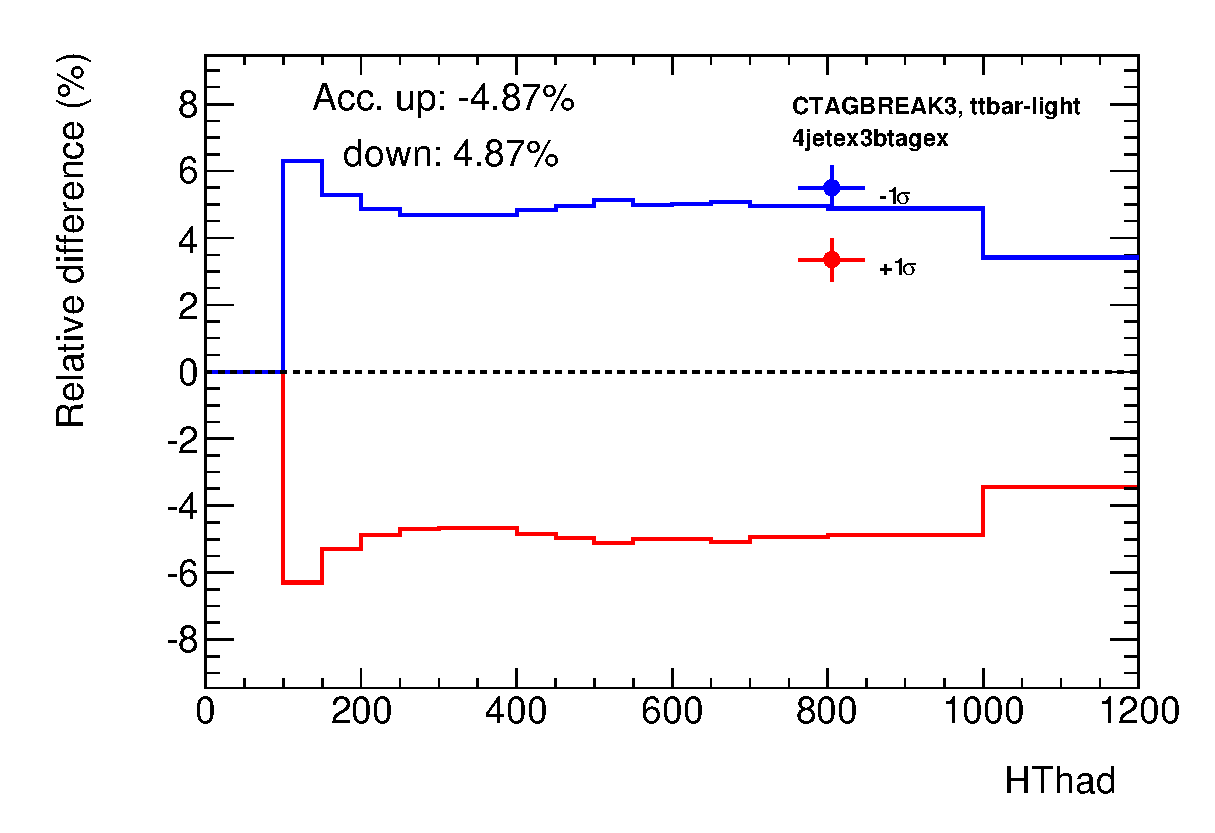
\includegraphics[width=\textwidth]{Analysis/Figures_ttH/ControlPlots/4jetex3btagex_ttbar-light_CTAGBREAK3.eps}
  \caption{} \label{fig:control_Ctag3}
  \end{subfigure} 
  \\
  \begin{subfigure}{0.47\textwidth}
     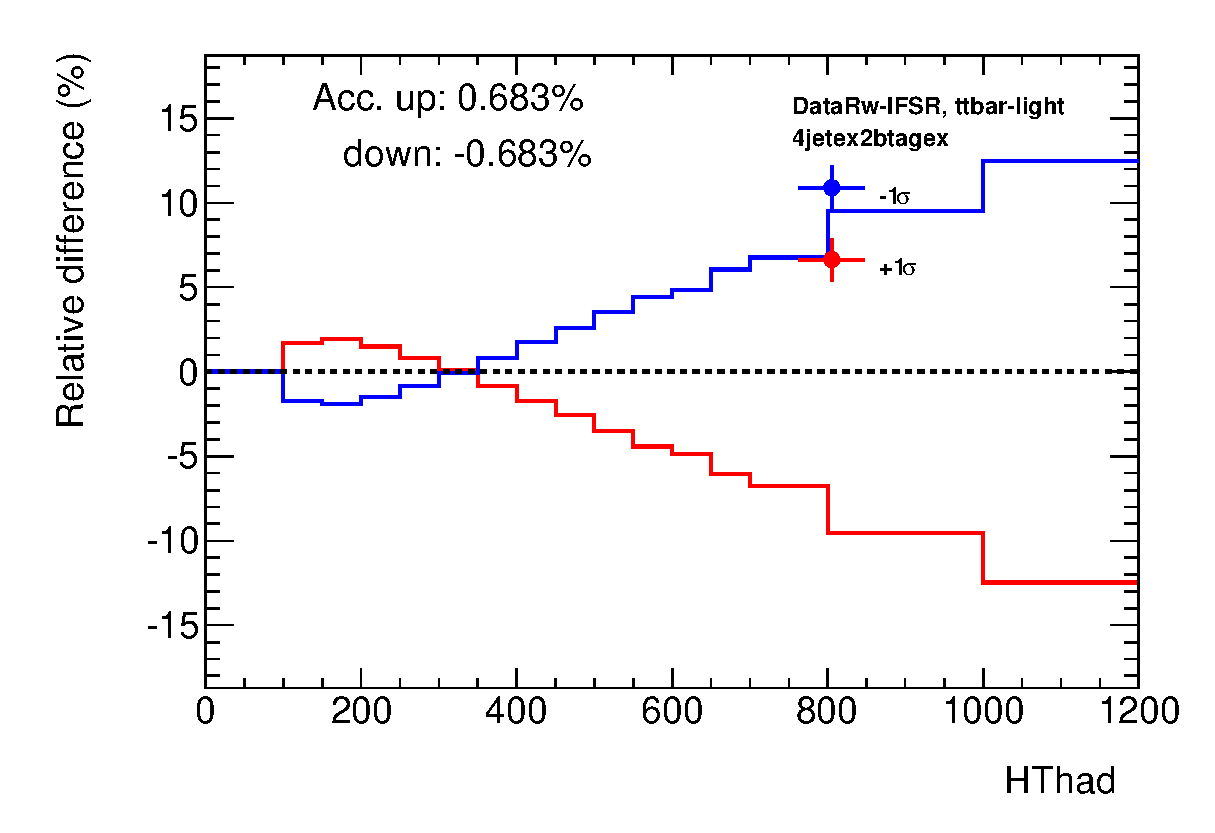
\includegraphics[width=\textwidth]{Analysis/Figures_ttH/ControlPlots/4jetex2btagex_ttbar-light_DataRw-IFSR.eps}
     \caption{} \label{fig:control_IFSR}
  \end{subfigure}
  \begin{subfigure}{0.47\textwidth}
     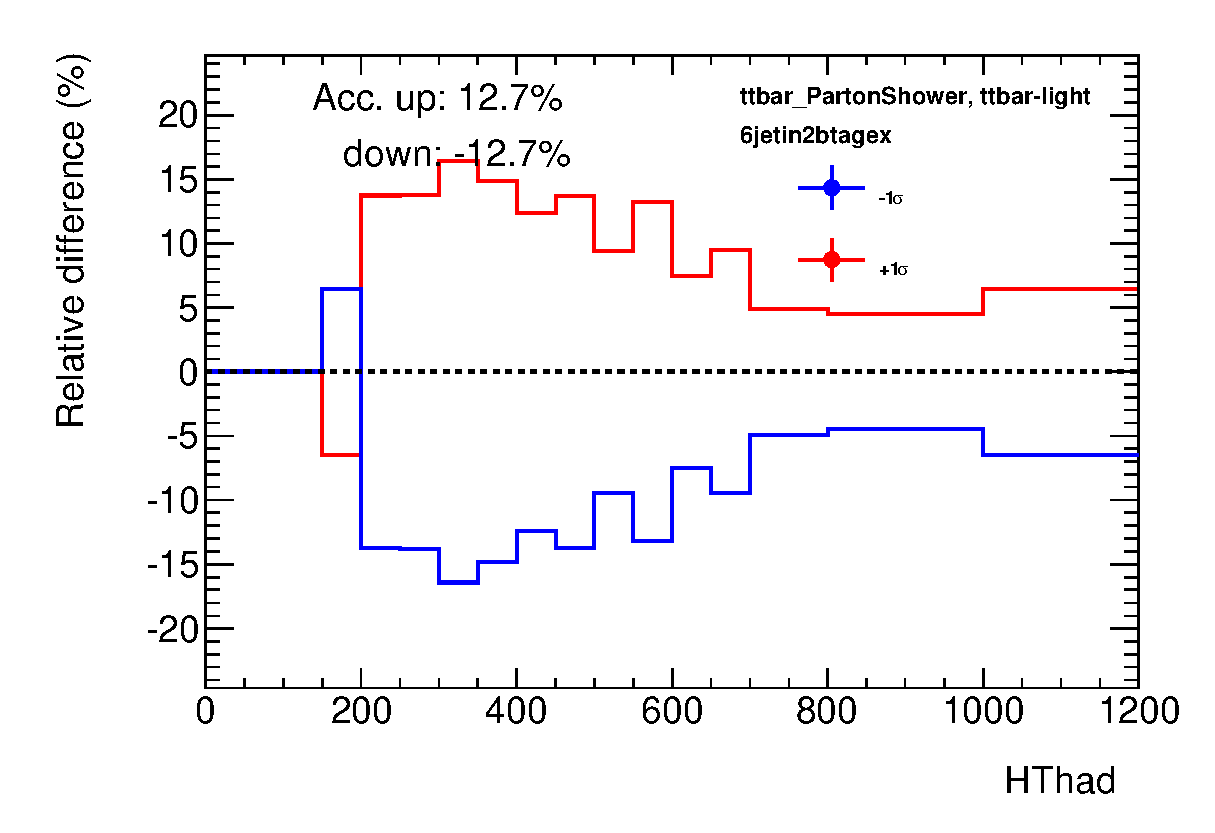
\includegraphics[width=\textwidth]{Analysis/Figures_ttH/ControlPlots/6jetin2btagex_ttbar-light_ttbar_PartonShower.eps}
  \caption{} \label{fig:control_PS}
  \end{subfigure} 
  \caption{Effect of different systematic uncertainties on the \ttbar+light jets sample: 
 (a) JetModel1 in the \fourtwo\ region, (b) JetFlavComp in the \fourtwo\ region, (c) 
  JER in the \fourtwo\ region, (d) $c$-tagging eigenvector 3 in the \fourthree\ region, (e) 
  DataRw-IFSR in the \fourtwo\ region and (f) ttbar PartonShower in the \sixtwo\ region.
}
\end{figure}

Other systematic uncertainties are not discussed since their pulls and constrains are less significant or they don't affect appreciably the sensitivity of the analysis. 

Figure~\ref{fig:ranking_ttH} demonstrates the effect of various systematic uncertainties on
the fitted value of $\mu$ and the constraints provided by the data. 
The largest effect arises
from the uncertainty in normalization of the irreducible \ttbb\ 
background, even after being reduced to half of 
the initial \unit[50]{\%}.
The \ttbb\ modeling uncertainties affecting the 
shape also have a significant effect on $\mu$, with four of them
among the highest-ranked systematic uncertainties.

\begin{figure}[!tpb]
\begin{center}
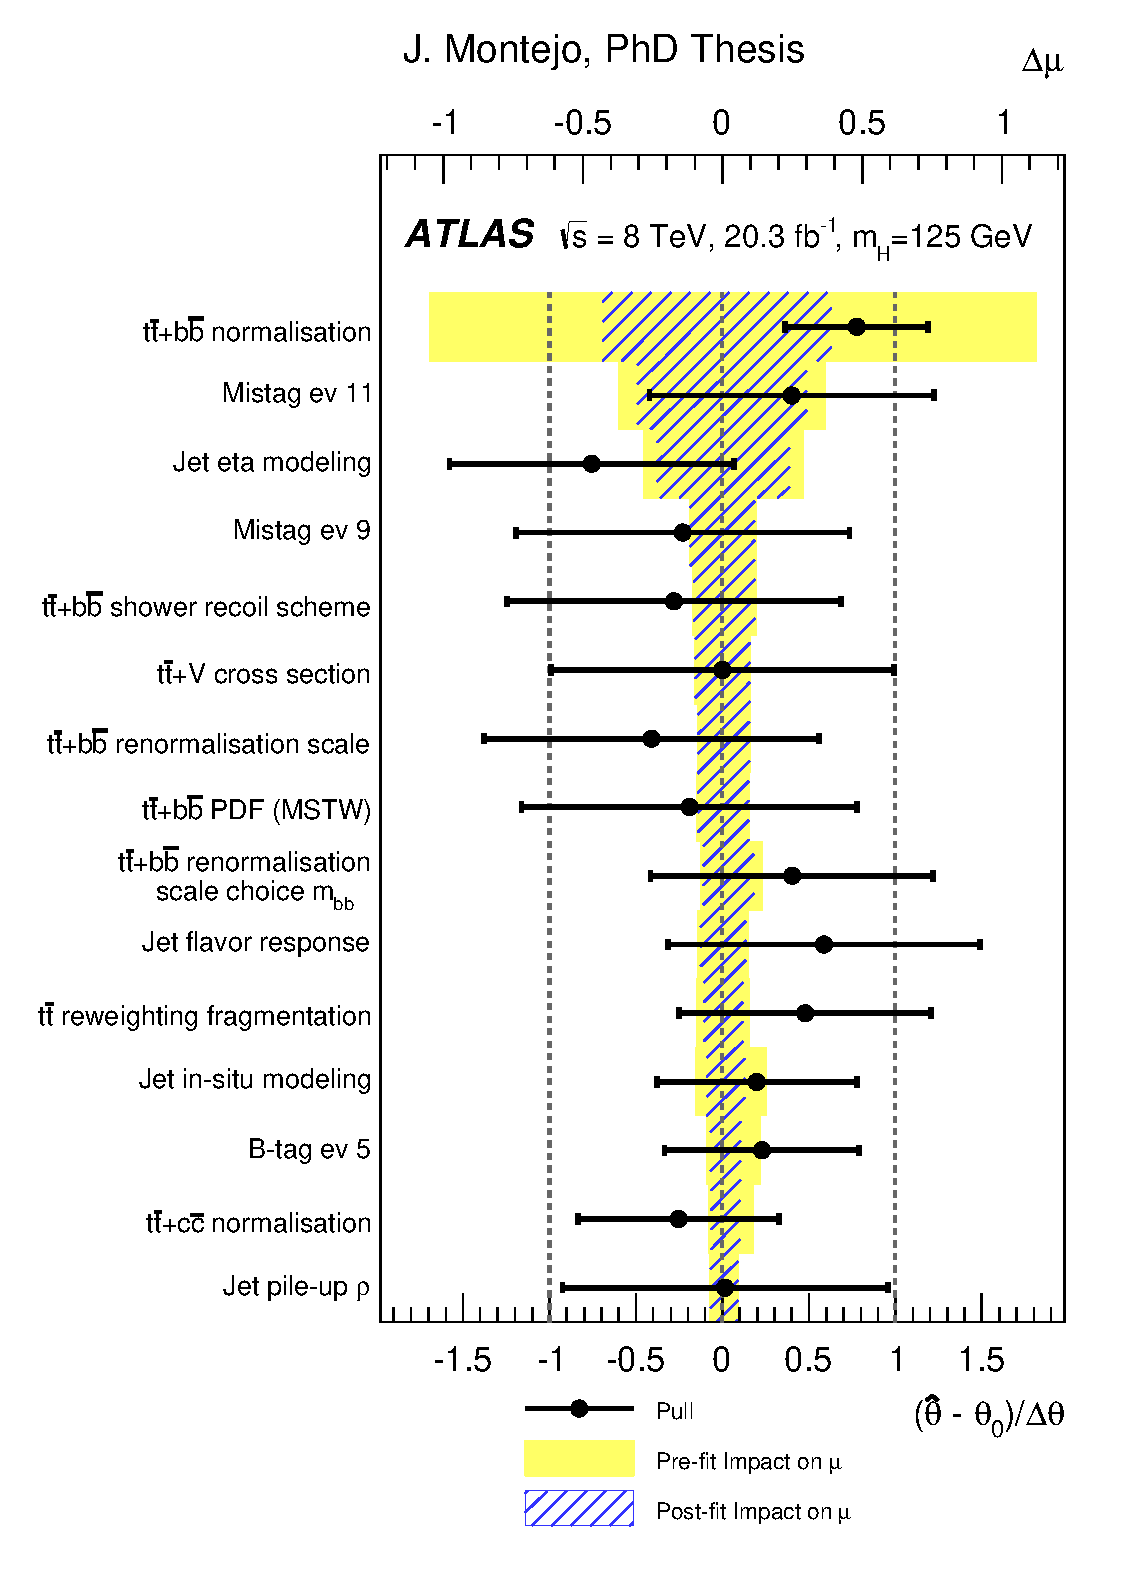
\includegraphics[width=0.7\textwidth]{Analysis/Figures_ttH/Dic09_AllSyst_lepjets_qcdsmooth_TRFscaled_pulls_125.eps}
\caption{ The fitted values of the 
NPs with the largest impact on the measured signal strength. The 
points, which are drawn conforming to the scale of the bottom axis, show the 
deviation of each of the fitted NPs, $\hat{\rm{\theta}}$, from 
$\rm{\theta_{0}}$, which is the nominal value of that NP, in units 
of the pre-fit standard deviation $\Delta\theta$. The error bars show the 
post-fit uncertainties, $\sigma_{\theta}$, which are close to 1 if the data do not provide 
any further constraint on that uncertainty. 
Conversely, a value of $\sigma_{\theta}$ much smaller than 1 indicates a significant 
reduction with respect to the original uncertainty. The NPs are 
sorted according to the post-fit effect of each on $\mu$ (hashed blue 
area) conforming to the 
scale of the top axis, with those with the largest impact at the top. }
\label{fig:ranking_ttH}
\end{center}
\end{figure}

\subsection{Limits on \ttH\ production}
Following the methodology discussed in chapter~\ref{chapter:Statistics}, the $p_0$-value is computed in order to test the compatibility of data with the background-only hypothesis. 
The observed (expected) $p$-value for the background-only hypothesis is \unit[15]{\%} (\unit[16]{\%}), which corresponds to an observed (expected)  significance of 1.0 (1.0) standard deviations. Since no significant excess over the background-only hypothesis is found, a \unit[95]{\%} CL upper limit can be set on the signal strength modifier. A signal 3.6 times larger than predicted by the SM is excluded at \unit[95]{\%} CL. A signal 2.6 times larger than the SM prediction is expected to be excluded if no SM \ttH\ process exists.

Figure~\ref{fig:SBordered_lj} summarizes post-fit event yields as a function of $\log_{10}(S/B)$, for all bins of the distributions used in the fit. The signal is normalized to the fitted value of the signal strength ($\mu = 1.2$) and a signal 3.6 times larger than predicted by the SM, which is excluded at \unit[95]{\%} CL, is also shown.

\begin{figure}[tbp!]
  \centering
  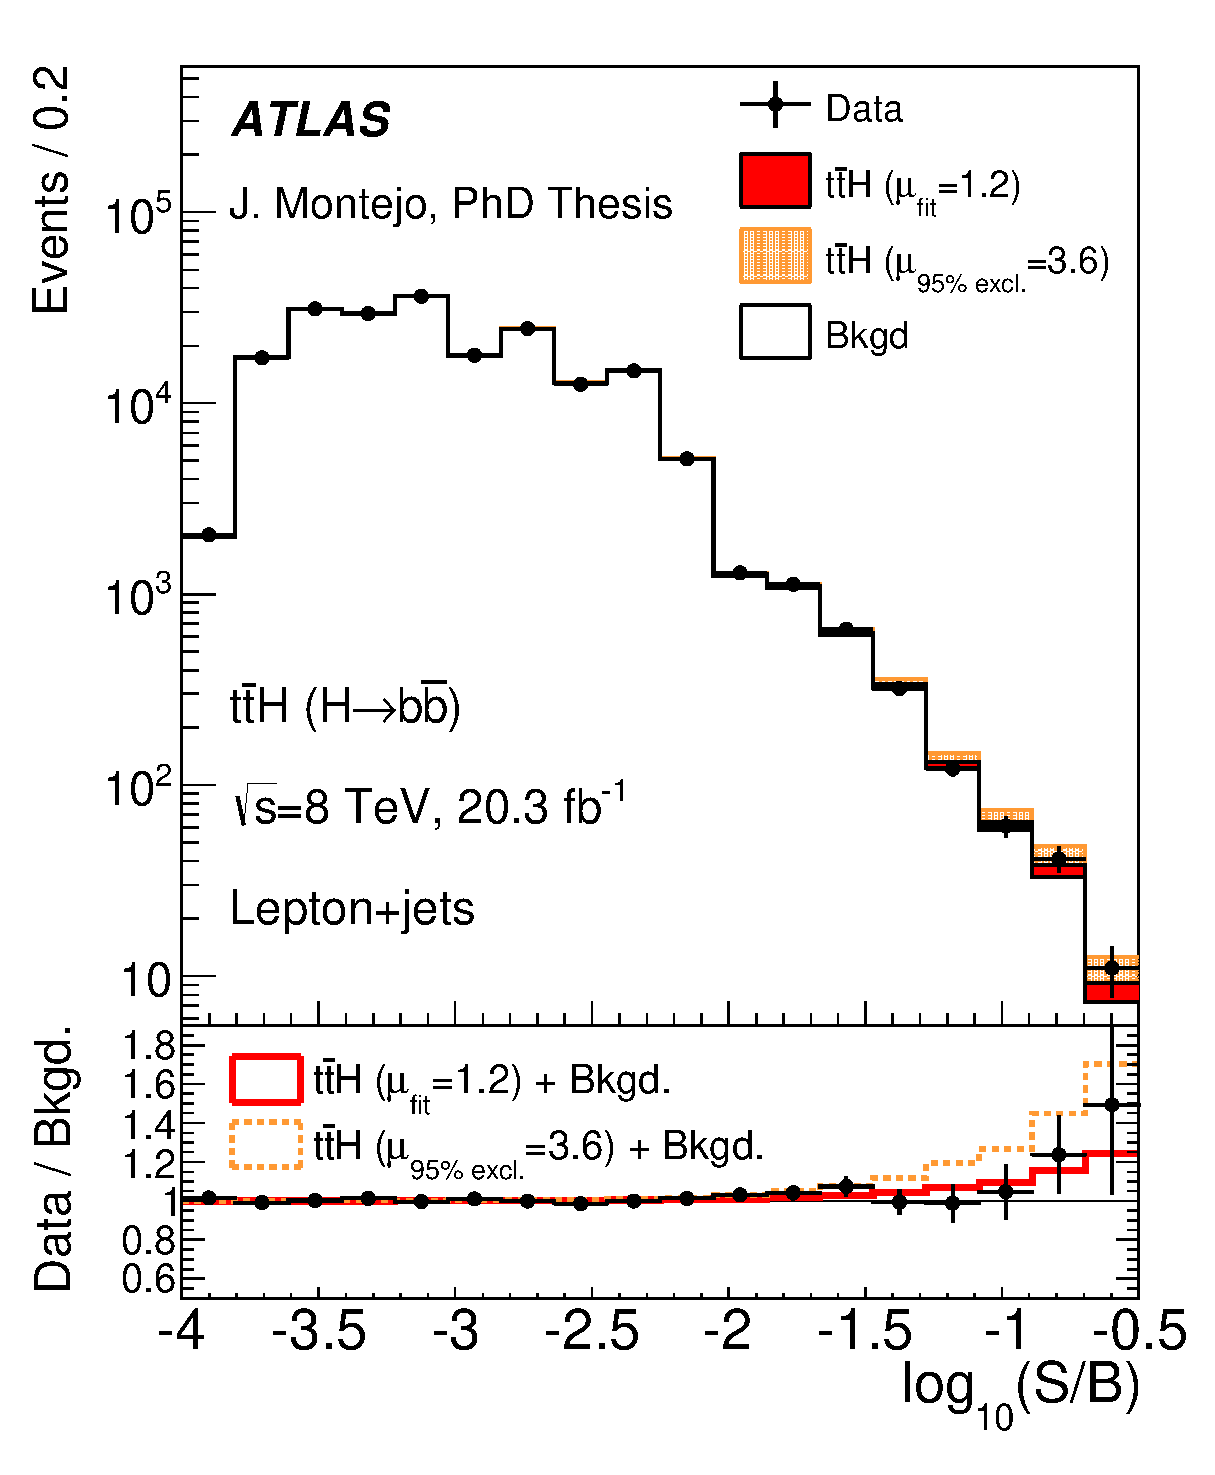
\includegraphics[width=0.7\textwidth]{Analysis/Figures_ttH/SBplot_lj_postfit.eps}
\caption{Event yields as a function of $\log_{10}(S/B)$, where $S$ 
(signal yield) and $B$ (background yield) are taken from the \hthad\ and NN output bin of each event.  Events in all fitted regions are included. 
The predicted background is obtained from the global signal-plus-background fit.  
The \tth\ signal is shown both for the best fit value ($\mu = 1.2$) and for the upper limit at 95\% CL ($\mu=3.6$).}
  \label{fig:SBordered_lj}
\end{figure}

\subsection{Analysis combination}
A complementary search for \ttH\ ($H \to \bbbar$) in the dileptonic channel has also been performed in ATLAS~\cite{Aad:2015gra}. The analysis procedure in the dileptonic channel is completely equivalent, and given that the datasets are orthogonal, the combination of both analyses can be performed.
A combined fit is performed to the nine regions of the single lepton search and six regions from the dilepton search. The result of the fit is shown in figure~\ref{fig:fit_ttH_combined}, and a good agreement in the fitted values is observed between the individual and the combined analyses.

\begin{figure}[!tp]
\begin{center}
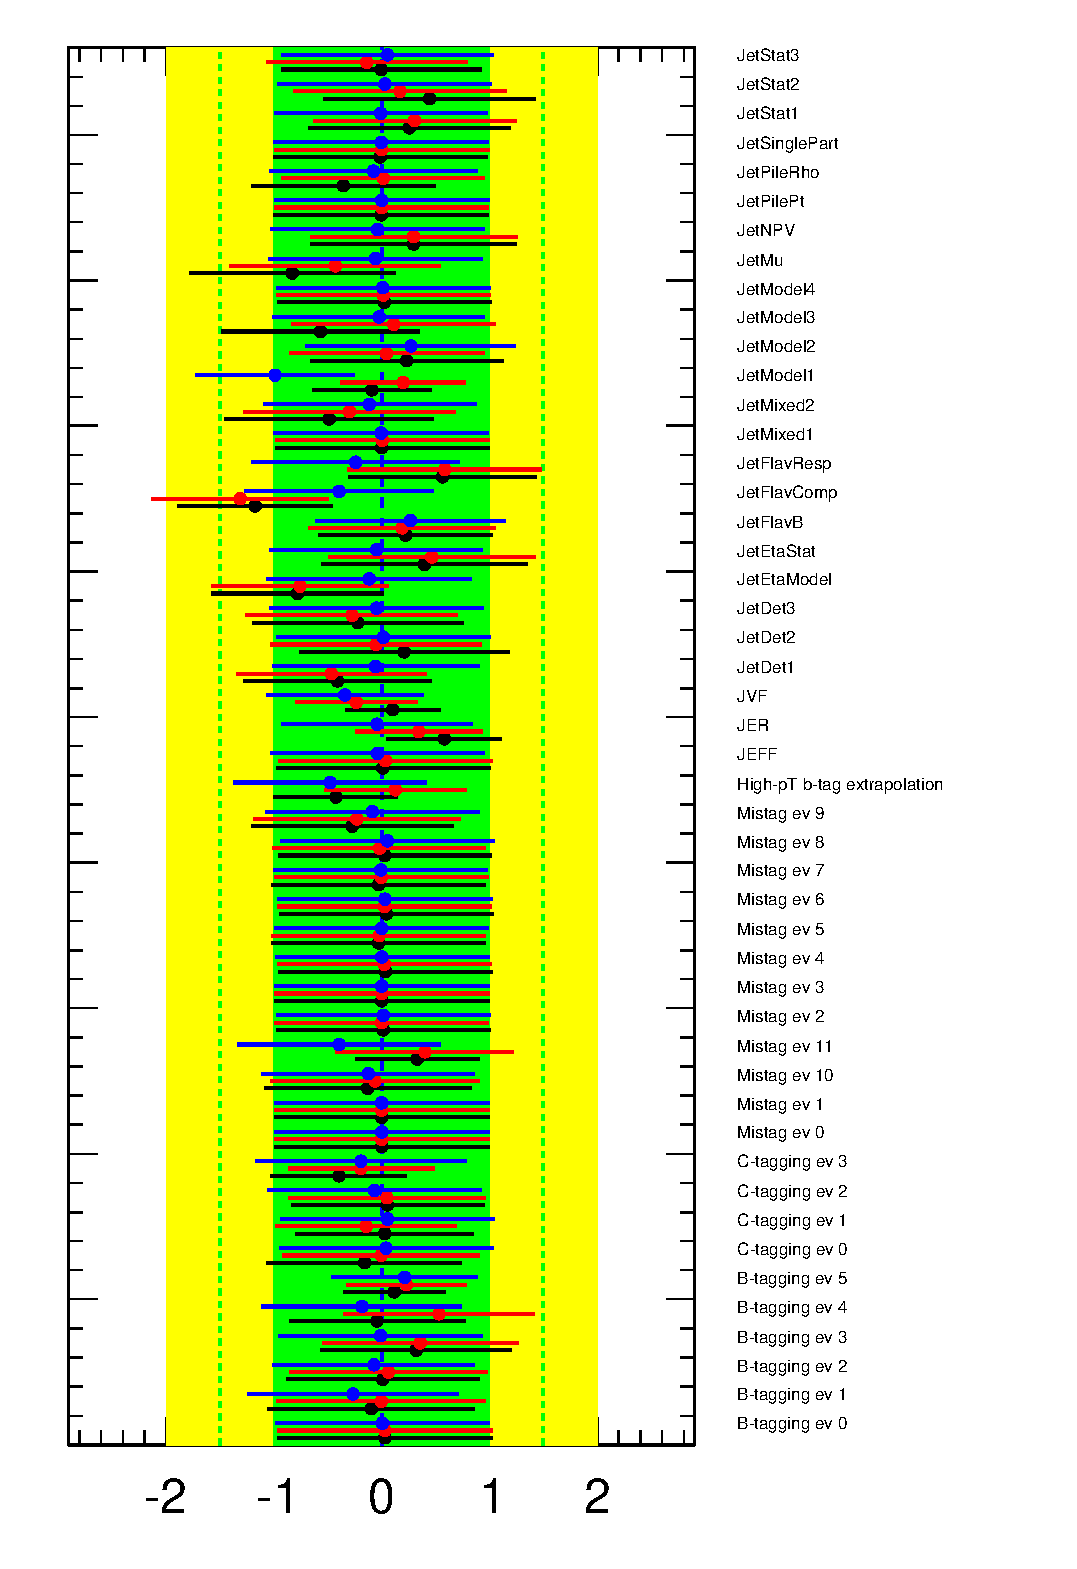
\includegraphics[trim=0cm 0cm 1.5cm 0cm, clip=true, width=0.49\textwidth]{Analysis/Figures_ttH/detectorUNCthreefit.eps}
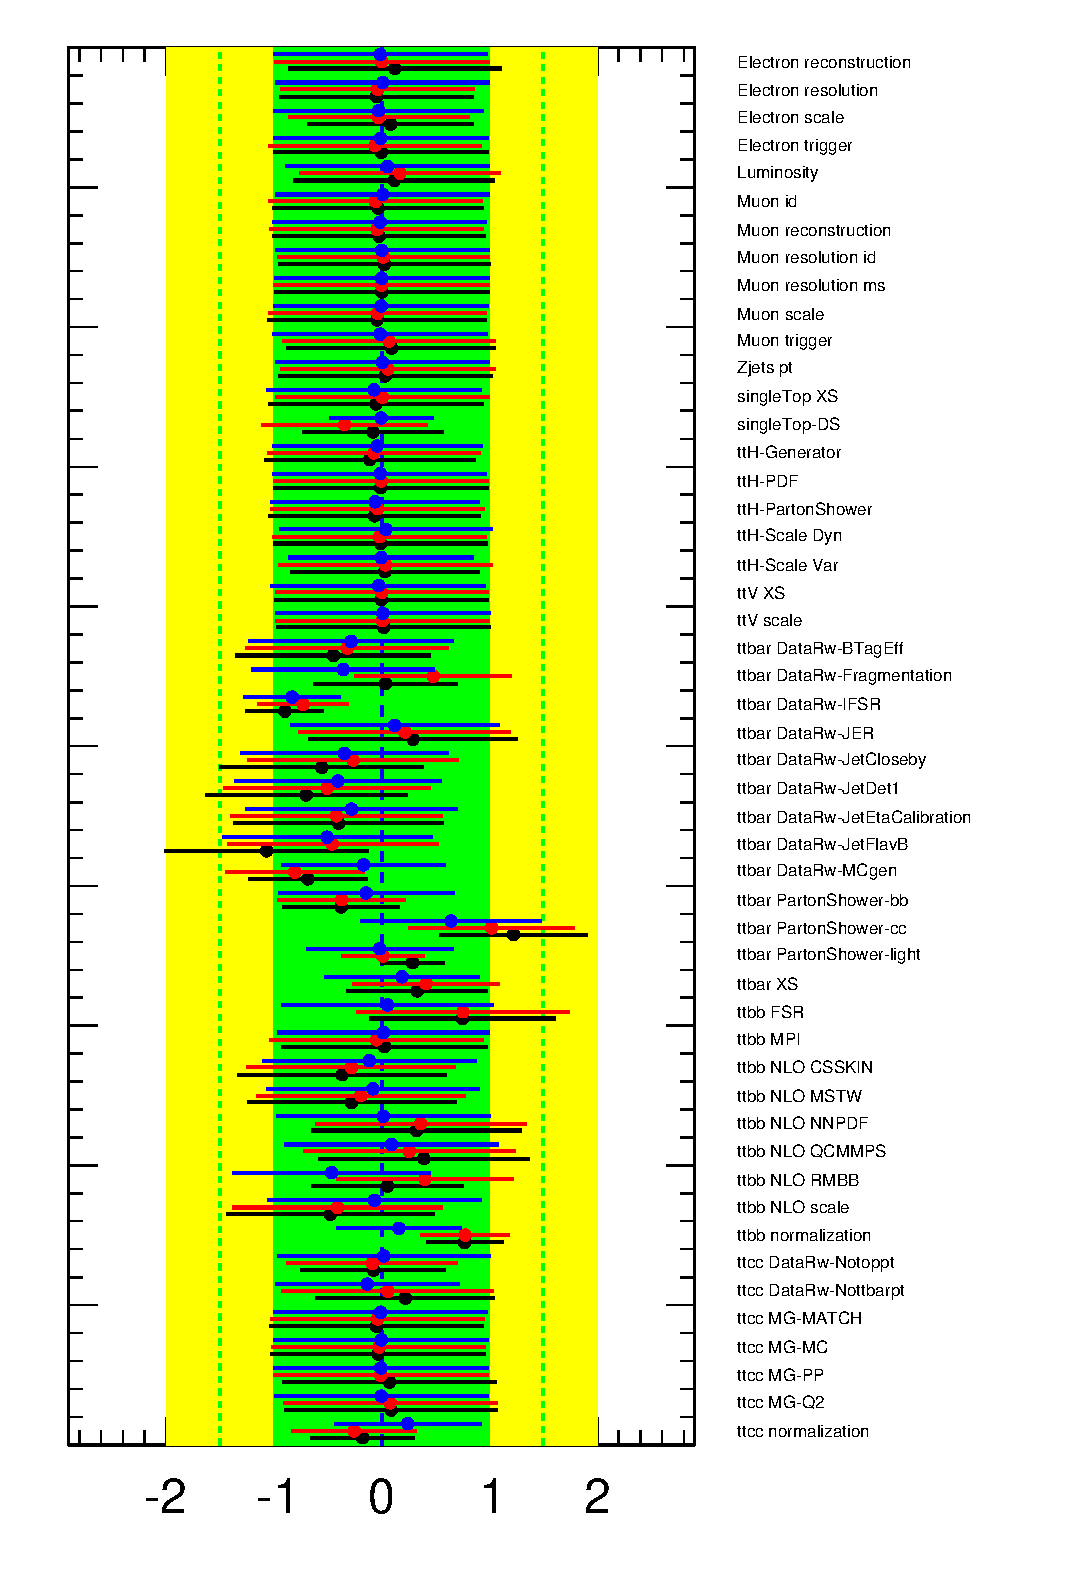
\includegraphics[trim=0cm 0cm 1.5cm 0cm, clip=true, width=0.49\textwidth]{Analysis/Figures_ttH/otherUNCthreefit.eps}
\caption{Fitted NPs under the signal-plus-background hypothesis for the three analyses (blue) dilepton, (red) lepton+jets and (black) combination. 
  Systematic uncertainties affecting only one of the analyses are not shown. A detailed description of the naming of the NPs can be found in appendix~\ref{app:glossary}.
}
\label{fig:fit_ttH_combined} 
\end{center}
\end{figure}

The observed $\mu$ values for the
single-lepton and dilepton searches, and their combination, are shown in figure~\ref{fig:fittedmu}. 
The fitted signal strength for 
the combined analysis is:
\begin{equation}
\mu  = 1.5 \pm 1.1~.
\end{equation} 
The observed (expected) significance of the signal is 1.4 (1.1)
standard deviations, which corresponds to an observed (expected) $p_0$-value of 8\% (15\%).   

The observed and expected limits
for both searches 
and their combination are shown in figure~\ref{fig:limits}. A signal 3.4 times larger than 
predicted by the SM is excluded at 95\% CL using the CL$_{\rm{s}}$ 
method. 
A signal 2.2 times larger than the SM prediction is expected to be excluded in the absence of the \ttH\ process, 
and 3.1 times larger than the SM prediction if the \ttH\ process is present with SM strength.  
The combination improves the expected sensitivity by \unit[15]{\%} respect to the single-lepton search alone.
The \unit[95]{\%} CL exclusion limits with their corresponding error bands are also summarized in table~\ref{tab:LimitsVSAnalysis}.

\begin{table}[!btp]
\begin{center}
  \makebox[\textwidth][c]{
\begin{tabular}{l|c|ccccc|c}
\toprule
\toprule
95\% CL upper limit     & Observed & $-2\sigma$  & $-1\sigma$  & Median    & $+1\sigma$  & $+2\sigma$ & Median ($\mu = 1$) \\

\midrule
Single lepton      &  3.6   &  1.4    & 1.9  &   2.6   & 3.7  & 4.9  & 3.6 \\
Dilepton           &  6.7   &  2.2    & 3.0  &   4.1   & 5.8  & 7.7  & 4.7 \\
\midrule
Combination        &  3.4   &  1.2    & 1.6  &   2.2   & 3.0  & 4.1  & 3.1 \\
\bottomrule
\bottomrule
\end{tabular}
}
\caption{\label{tab:LimitsVSAnalysis} Observed and expected
(median, for the background-only hypothesis) 95\% CL upper limits on
$\sigma(t\bar{t}H)$ relative to the SM prediction, for the individual channels as well as their
combination, assuming $m_H=125\gev$. 
%The 68\% and 95\% confidence intervals around the expected limits under the background-only hypothesis are also provided, denoted by $\pm 1 \sigma$ and $\pm 2 \sigma$, respectively.  
The expected (median) 95\% CL upper limits assuming the SM prediction for $\sigma(t\bar{t}H)$ are shown in the last column. }
\end{center}
\end{table}

Finally, figure~\ref{fig:logSBplot} summarizes the post-fit event yields as a function of $\log_{10}(S/B)$, 
for all bins of the distributions used in the combined fit of the single-lepton and dilepton channels. 


\begin{figure}[!tpb]
\begin{center}
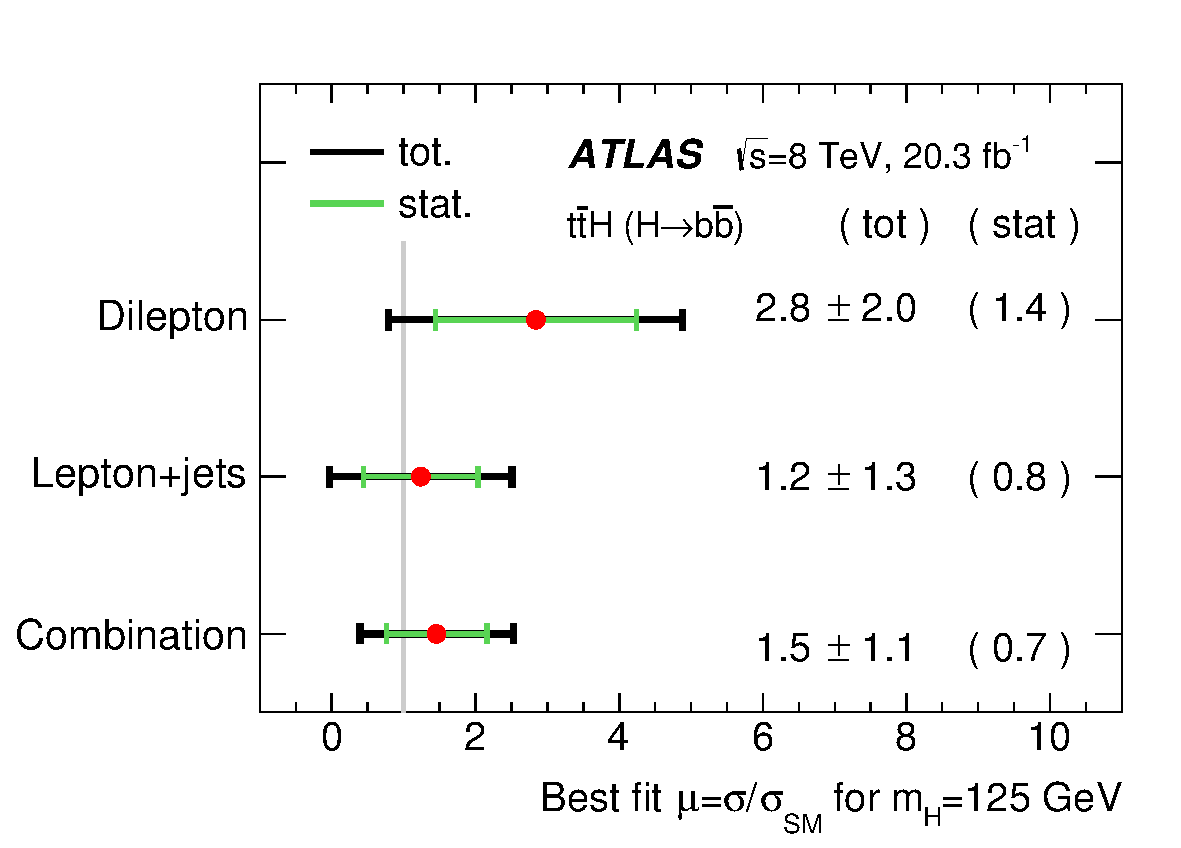
\includegraphics[width=0.7\textwidth]{Analysis/Figures_ttH/MuPlot_Dic09.pdf}
\caption{The fitted values of the signal strength and their uncertainties for 
the individual channels and their 
combination.  The green line shows the statistical
uncertainty on the signal strength.}
\label{fig:fittedmu} 
\end{center}
\end{figure}

\begin{figure}[!tpb]
\begin{center}
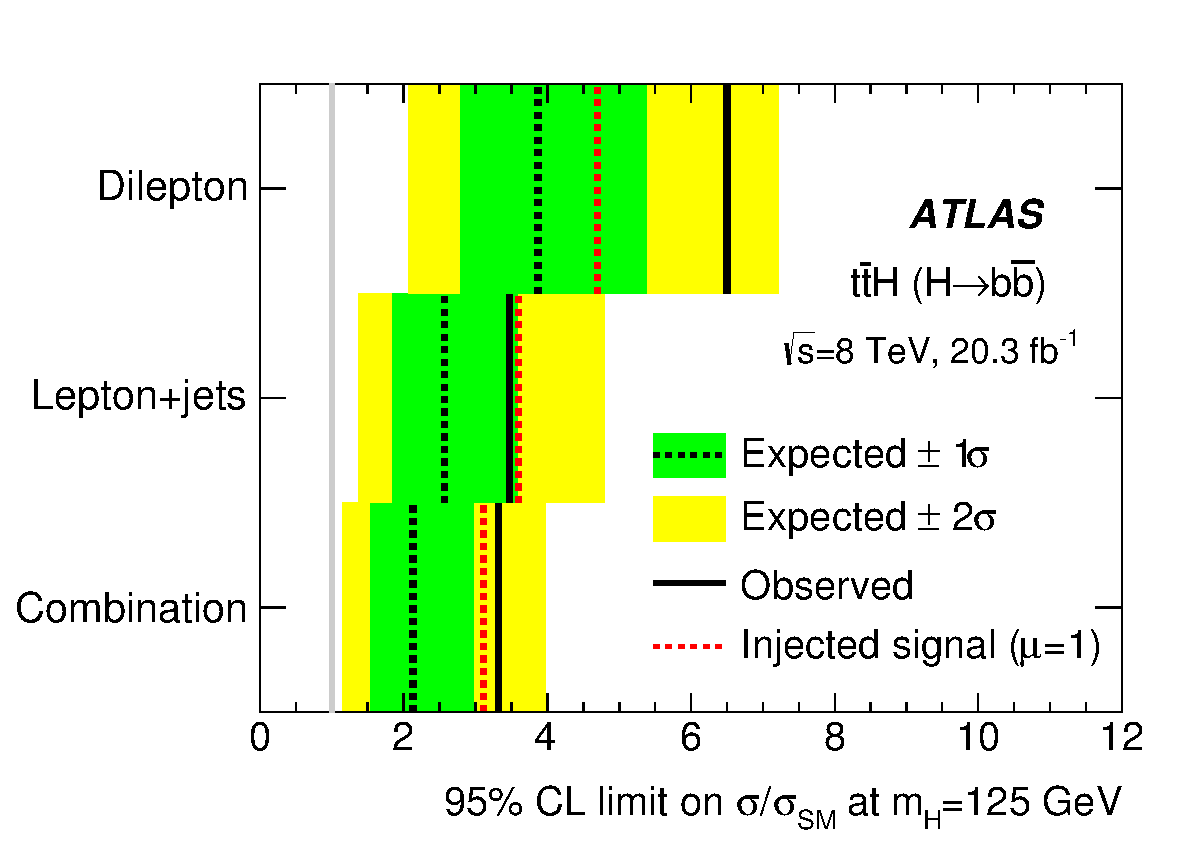
\includegraphics[width=0.7\textwidth]{Analysis/Figures_ttH/LimitPlot_Dic09.pdf}
\caption{95\% CL upper limits on $\sigma(t\bar{t}H)$ relative to the SM prediction, $\sigma/\sigma_{\mathrm{SM}}$, for the individual 
channels as well as their combination. The observed 
limits (solid lines) are compared
to the expected (median) limits under the background-only hypothesis and under
the signal-plus-background hypothesis assuming the SM prediction 
for $\sigma(t\bar{t}H)$ and pre-fit prediction for the background.
The surrounding shaded bands correspond to the 68\% and 95\% confidence 
intervals around the expected limits under the background-only hypothesis, 
denoted by $\pm 1 \sigma$ and $\pm 2 \sigma$, respectively. }
\label{fig:limits} 
\end{center}
\end{figure}	


\subsection{Comparison with other analyses}
Searches for the \ttH\ process have also been performed in ATLAS in the diphoton~\cite{Aad:2014lma} and multilepton~\cite{ATLAS-CONF-2015-006} final states. 
The expected exclusion limits are 4.9 and 2.4 times the SM prediction, respectively.
The combination of the three analyses: \bbbar, diphoton and multilepton, has also been performed in order to search for possible deviations in the Higgs couplings~\cite{ATLAS-CONF-2015-007}, yielding an expected sensitivity of 1.4 times the SM prediction.
The individual fitted signal strengths and the combination of the three analyses are summarized in figure~\ref{fig:ttH_combo}.
\begin{figure}[!tpb]
\begin{center}
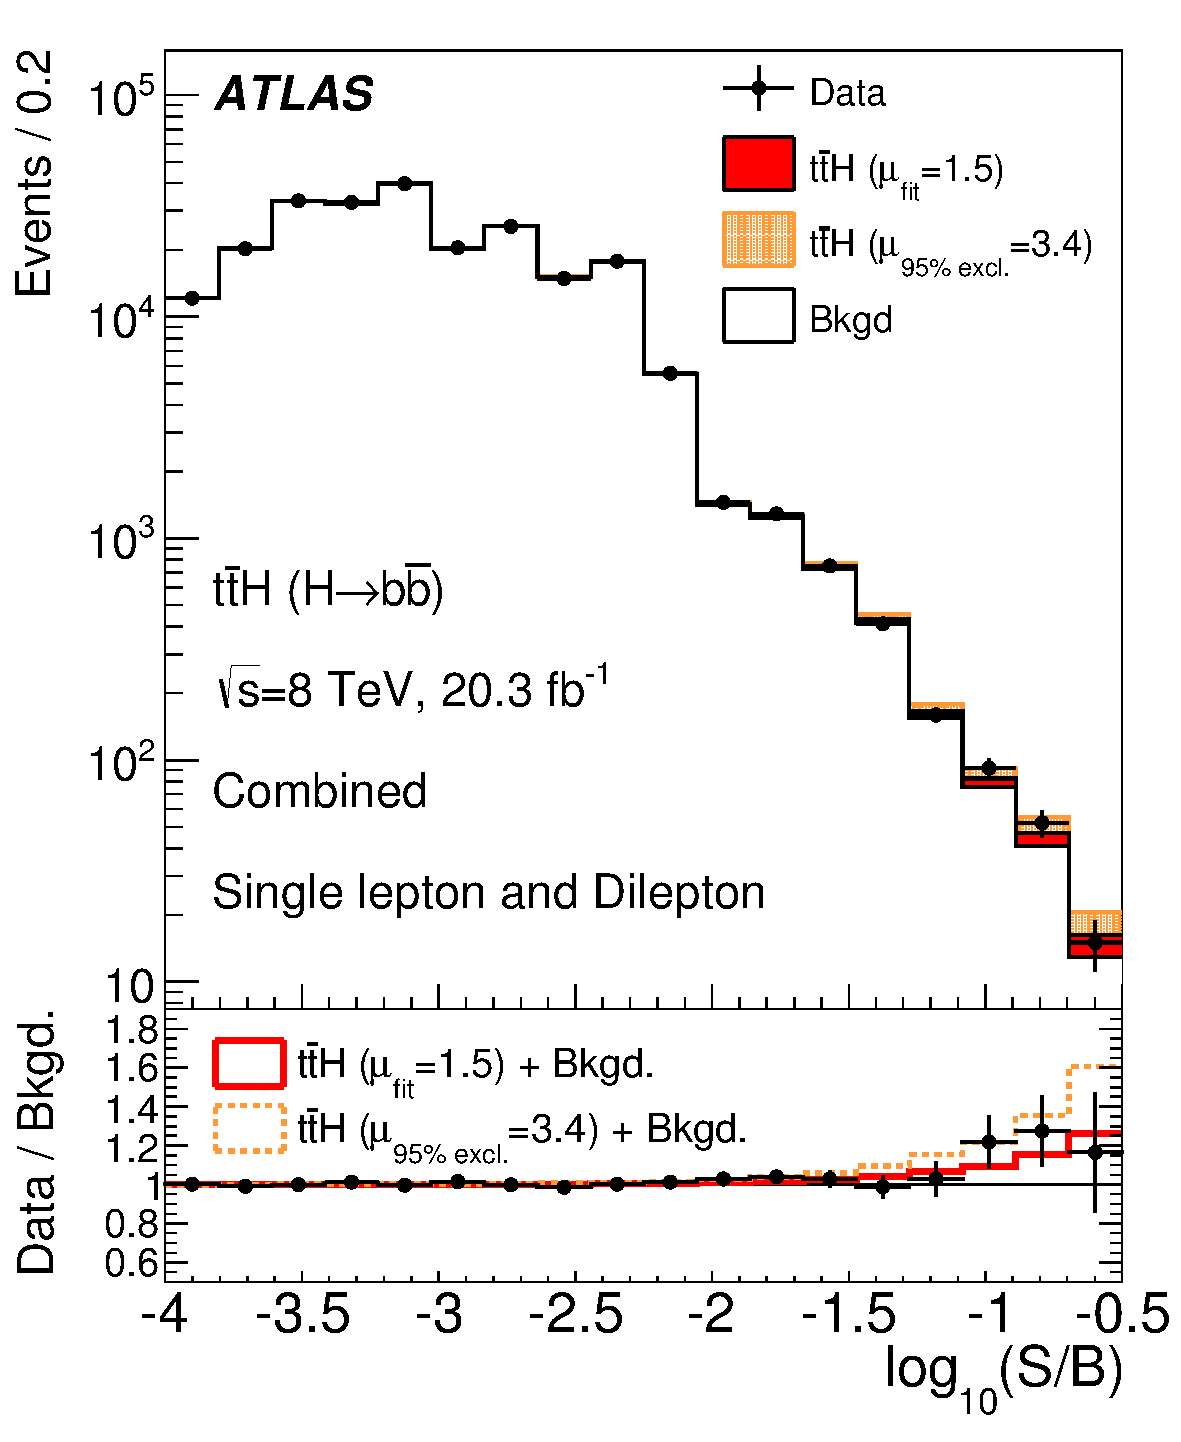
\includegraphics[trim=0cm 0.4cm 0cm 0.8cm, clip=true, width=0.55\textwidth]{Analysis/Figures_ttH/SBplot_postfit.pdf}
\caption{Event yields as a function of $\log_{10}(S/B)$, where $S$ 
(signal yield) and $B$ (background yield) are taken from the \hthad, 
\htlep, and NN output bin of each event.  Events in all fitted regions are included. 
The predicted background is obtained from the global signal-plus-background fit.  
The \tth\ signal is shown both for the best fit value ($\mu = 1.5$) and for the upper limit at 95\% CL ($\mu=3.4$).}
\label{fig:logSBplot}
\end{center}
\vspace{-1.2cm}
\end{figure}
\begin{figure}[bht!]
  \centering
  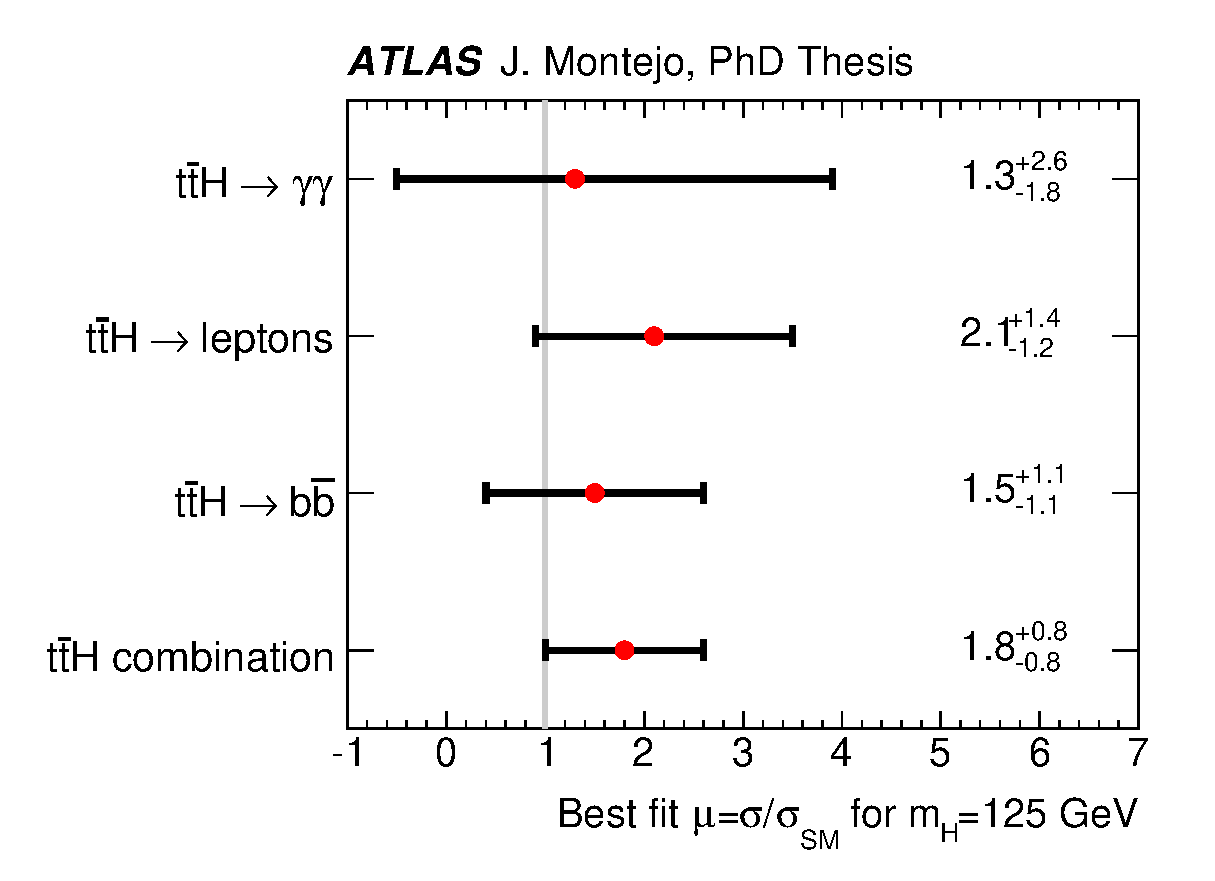
\includegraphics[trim=0cm 0.2cm 0cm 0.5cm, clip=true, width=0.65\textwidth]{Analysis/Figures_ttH/MuPlot_ttH_combo.eps}
  \caption{Fitted signal strength in the individual \ttH\ searches and their combination.}
  \label{fig:ttH_combo}
\end{figure}

A search for the 
associated production of the Higgs boson with a top-quark pair using  
several Higgs decay modes (including \htobb) has been published  
by the CMS Collaboration~\cite{CMS8TeVttH} quoting a ratio of the 
measured \tth\ signal \xsec\ to the SM expectation 
for a Higgs boson mass of \unit[125.6]{\gev} of $\mu = 2.8 \pm 1.0$.

The matrix element method was also used for a search in the \ttH, \htobb\ channel by the
CMS experiment~\cite{CMSMEM}. A second discriminating variable was defined to separate \ttHF\ from \ttbar+light-jets. The signal is extracted via a two-dimensional fit to both discriminants and the fitted signal strength is: $\mu = 1.2^{+1.6}_{-1.5}$.

The analysis described in this dissertation is the most sensitive search to date for the \ttH\ process.

\clearpage
